\documentclass[10pt]{beamer}
%Information to be included in the title page:
\title{Taller de Supervivencia en Shell}
\author{RoboTech URJC}
\institute[]{URJC}
\date{2023}
\usepackage{hyperref}
\hypersetup{ colorlinks=true,%linkcolor=black,
	urlcolor=blue,}
\usetheme{Madrid}
\usecolortheme{beaver}
\usepackage{graphicx} %LaTeX package to import graphics
\graphicspath{{images/}} %configuring the graphicx package
\logo{
\includegraphics[width=0.25\textwidth]{logo}
\includegraphics[scale=0.2]{robotech}}

\begin{document}
	
	\frame{\titlepage}
	
	\begin{frame}
		\frametitle{Licencia}
		(cc) 2018 Grupo de Sistemas y Comunicaciones.
		\newline
		\newline
		(cc) 2023 Robotech.
		\newline
		\newline
		Algunos derechos reservados. Este trabajo se entrega bajo la licencia Creative Commons Reconocimiento –NoComercial - SinObraDerivada (by-nc-nd). Para obtener la licencia completa, véase:
		\newline
		\newline
		http://creativecommons.org/licenses/by-sa/2.1/es.También puede solicitarse a Creative Commons, 559 Nathan
		\newline
		\newline
		Abbott Way, Stanford, California 94305, USA.
	\end{frame}
	
	\begin{frame}
		\frametitle{¿Quiénes somos?}
		\begin{itemize}
			\item Javier Izquierdo Hernández: \\
			Estudiante de ingeniería robótica software (3º año).\\
			Github: \url{https://github.com/javizqh}
			\item Iker Peral del Pino: \\
			Estudiante de ingeniería robótica software (3º año).
		\end{itemize}
		\vspace{20pt}
		\begin{center}
			
\includegraphics[width=15 pt]{twitter} \hspace{5 pt}
\includegraphics[width=15 pt]{instagram}\hspace{10 pt} @robotech\_urjc\\
			
			
\includegraphics[width=15 pt]{mail} \hspace{10 pt} robotechurjc@gmail.com
		\end{center}
	\end{frame}
	
	\begin{frame}
		\frametitle{¿Qué es la Shell?}
		Programa que te deja ejecutar commandos, por ejemplo dash, bash, zsh, etc…	\\
		Ejemplo:
		\textbf{username}@\textbf{hostname}:\textbf{where} \textbf{\$ ó \#} echo hola\\
		\begin{itemize}
			\item El username puede ser tu usuario o root.
			\item El hostname es el nombre de tu ordenador.
			\item Where indica el directorio actual.
			\item \$ indica si el usuario es un usuario normal.
			\item \# indica si el usuario es root.
		\end{itemize}
		Todo esto también se puede configurar al gusto.\\
	\end{frame}

	\begin{frame}
		\frametitle{Estructura de un Comando}
		El comando es el programa a ejecutar con sus argumento(s) y flag(s).\\
		Por ejemplo: \textbf{ls} (comando) \textbf{-a} (flag) \textbf{prueba/} (argumento)		
		\begin{center}
			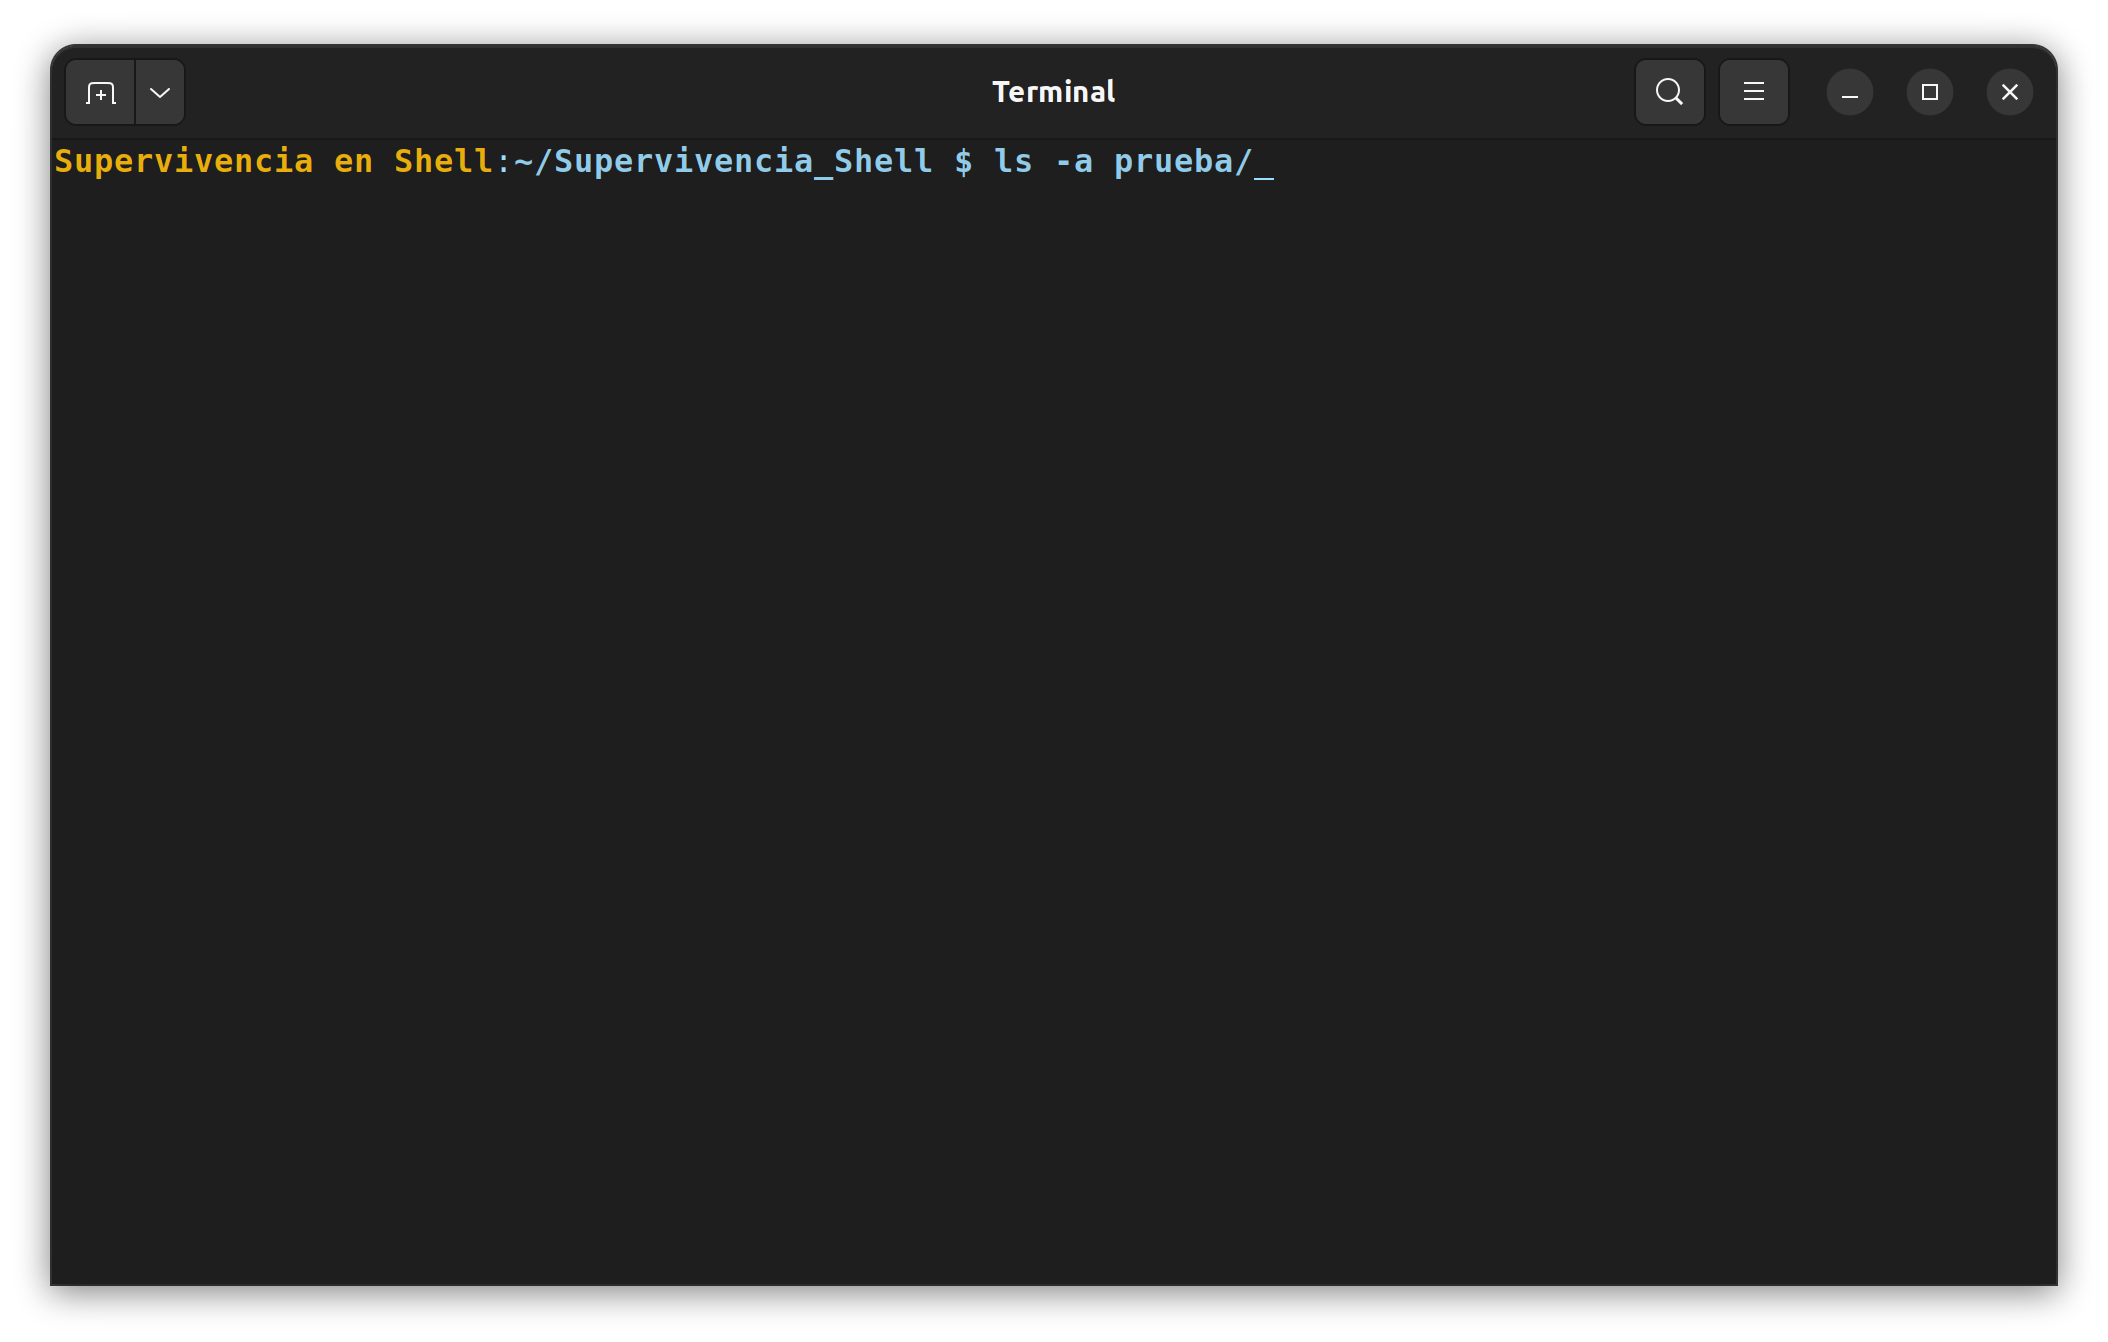
\includegraphics[width=0.60\textwidth]{cmd}
		\end{center}
	\end{frame}
	
	\begin{frame}
		\frametitle{El Manual: man}
		\begin{alertblock}{Muestra las páginas de manual.}
			man sección asunto;    Ejemplo: man 1 ls
		\end{alertblock}
		\begin{center}
			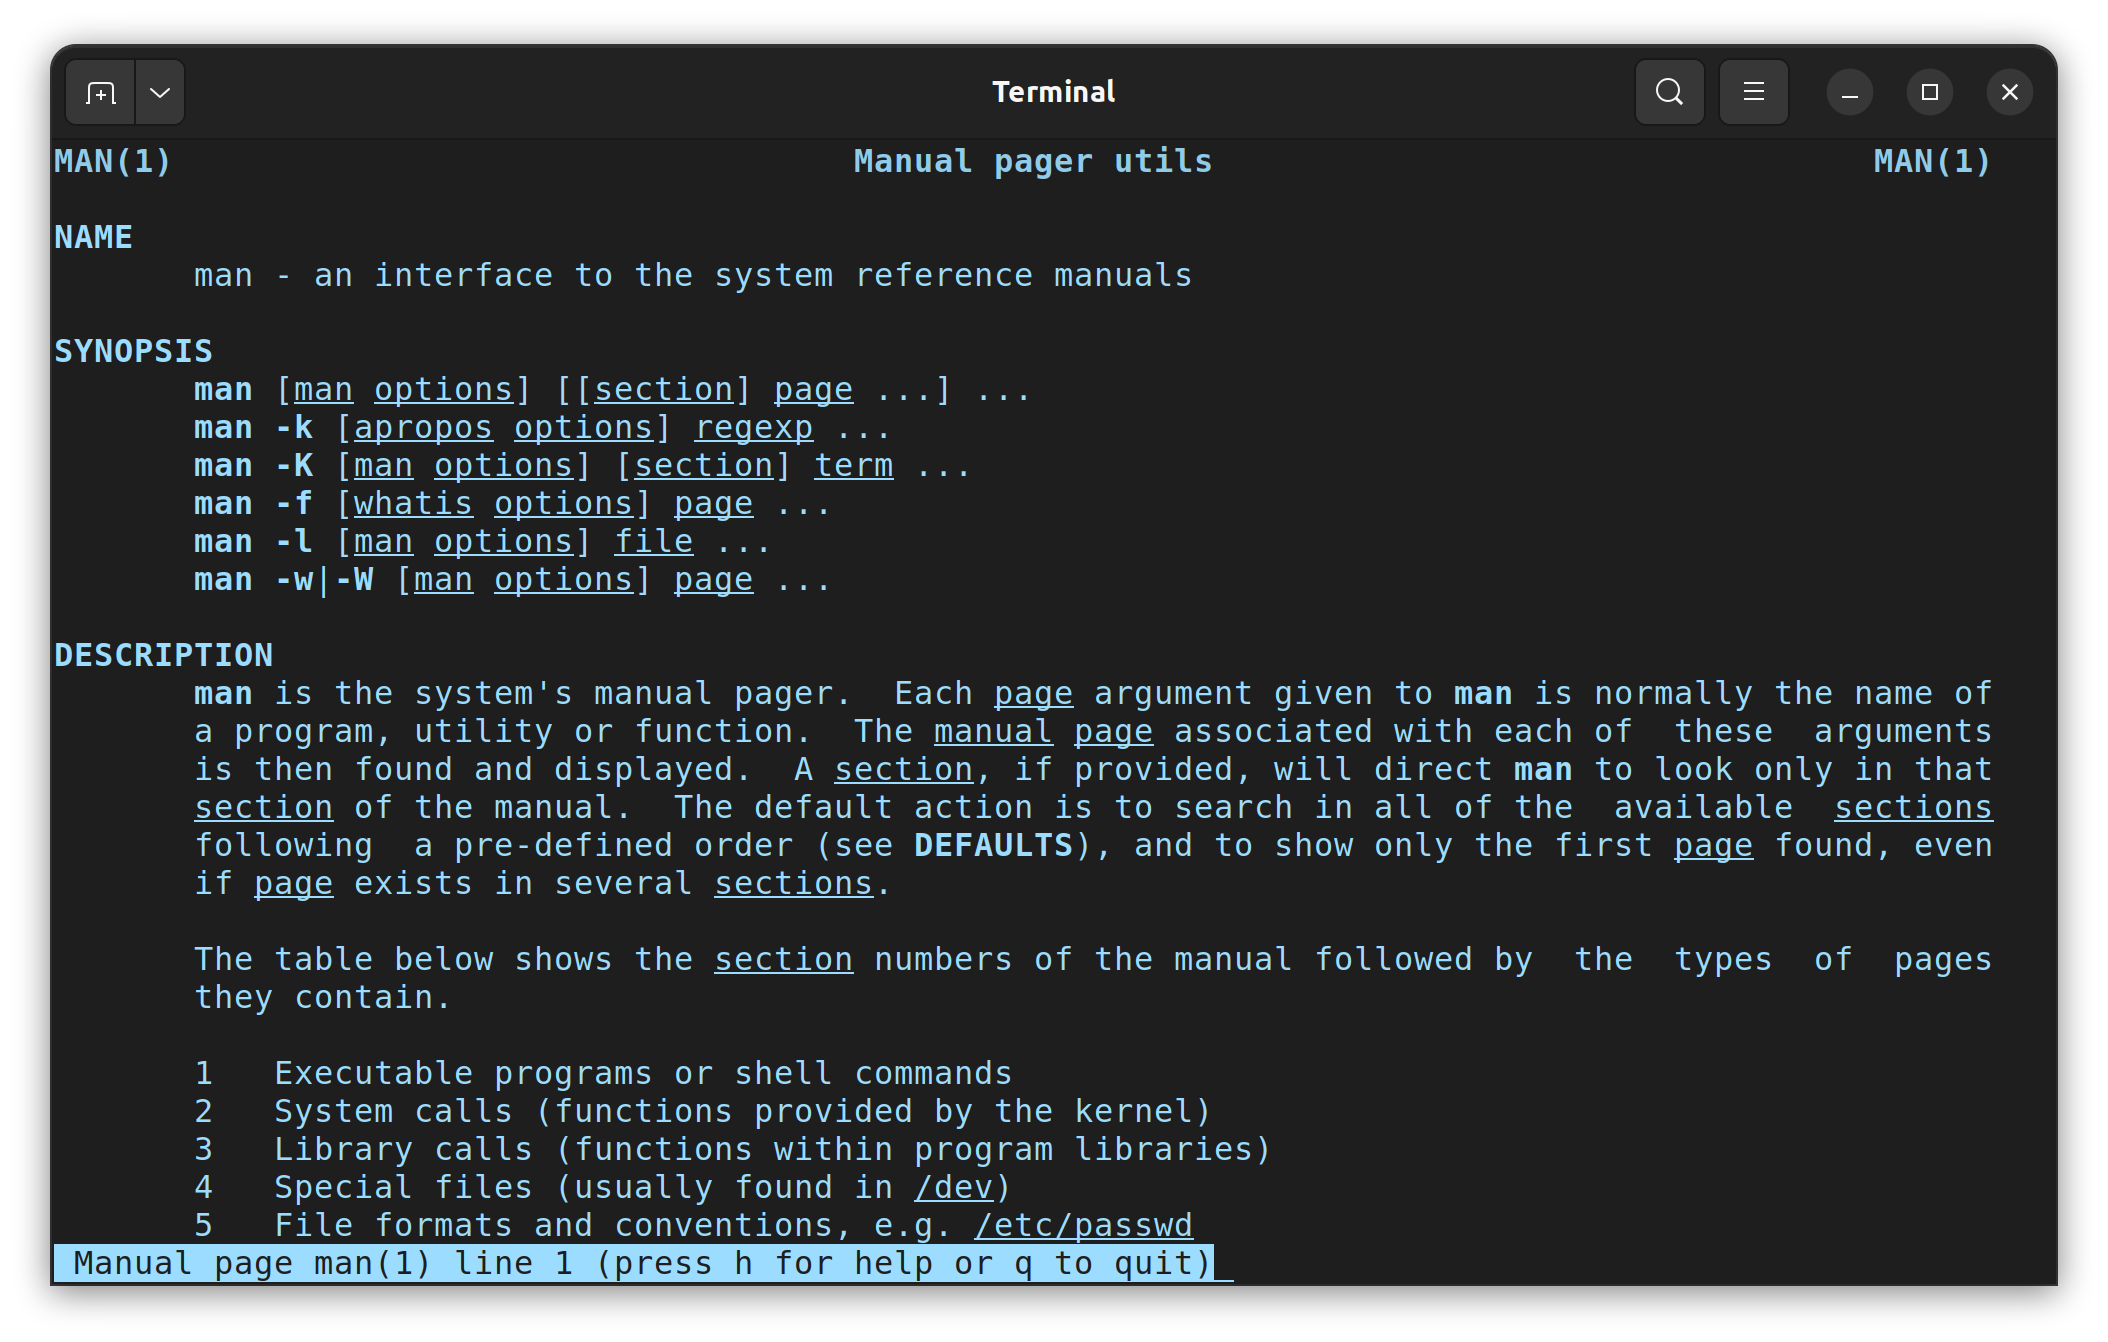
\includegraphics[width=0.55\textwidth]{man}
		\end{center}
	\end{frame}
	
	\begin{frame}
		\frametitle{El Manual: apropos}
		\begin{alertblock}{Buscar sobre el nombre de una pagina de manual y su descripción.}
			apropos keyword
		\end{alertblock}
		\begin{center}
			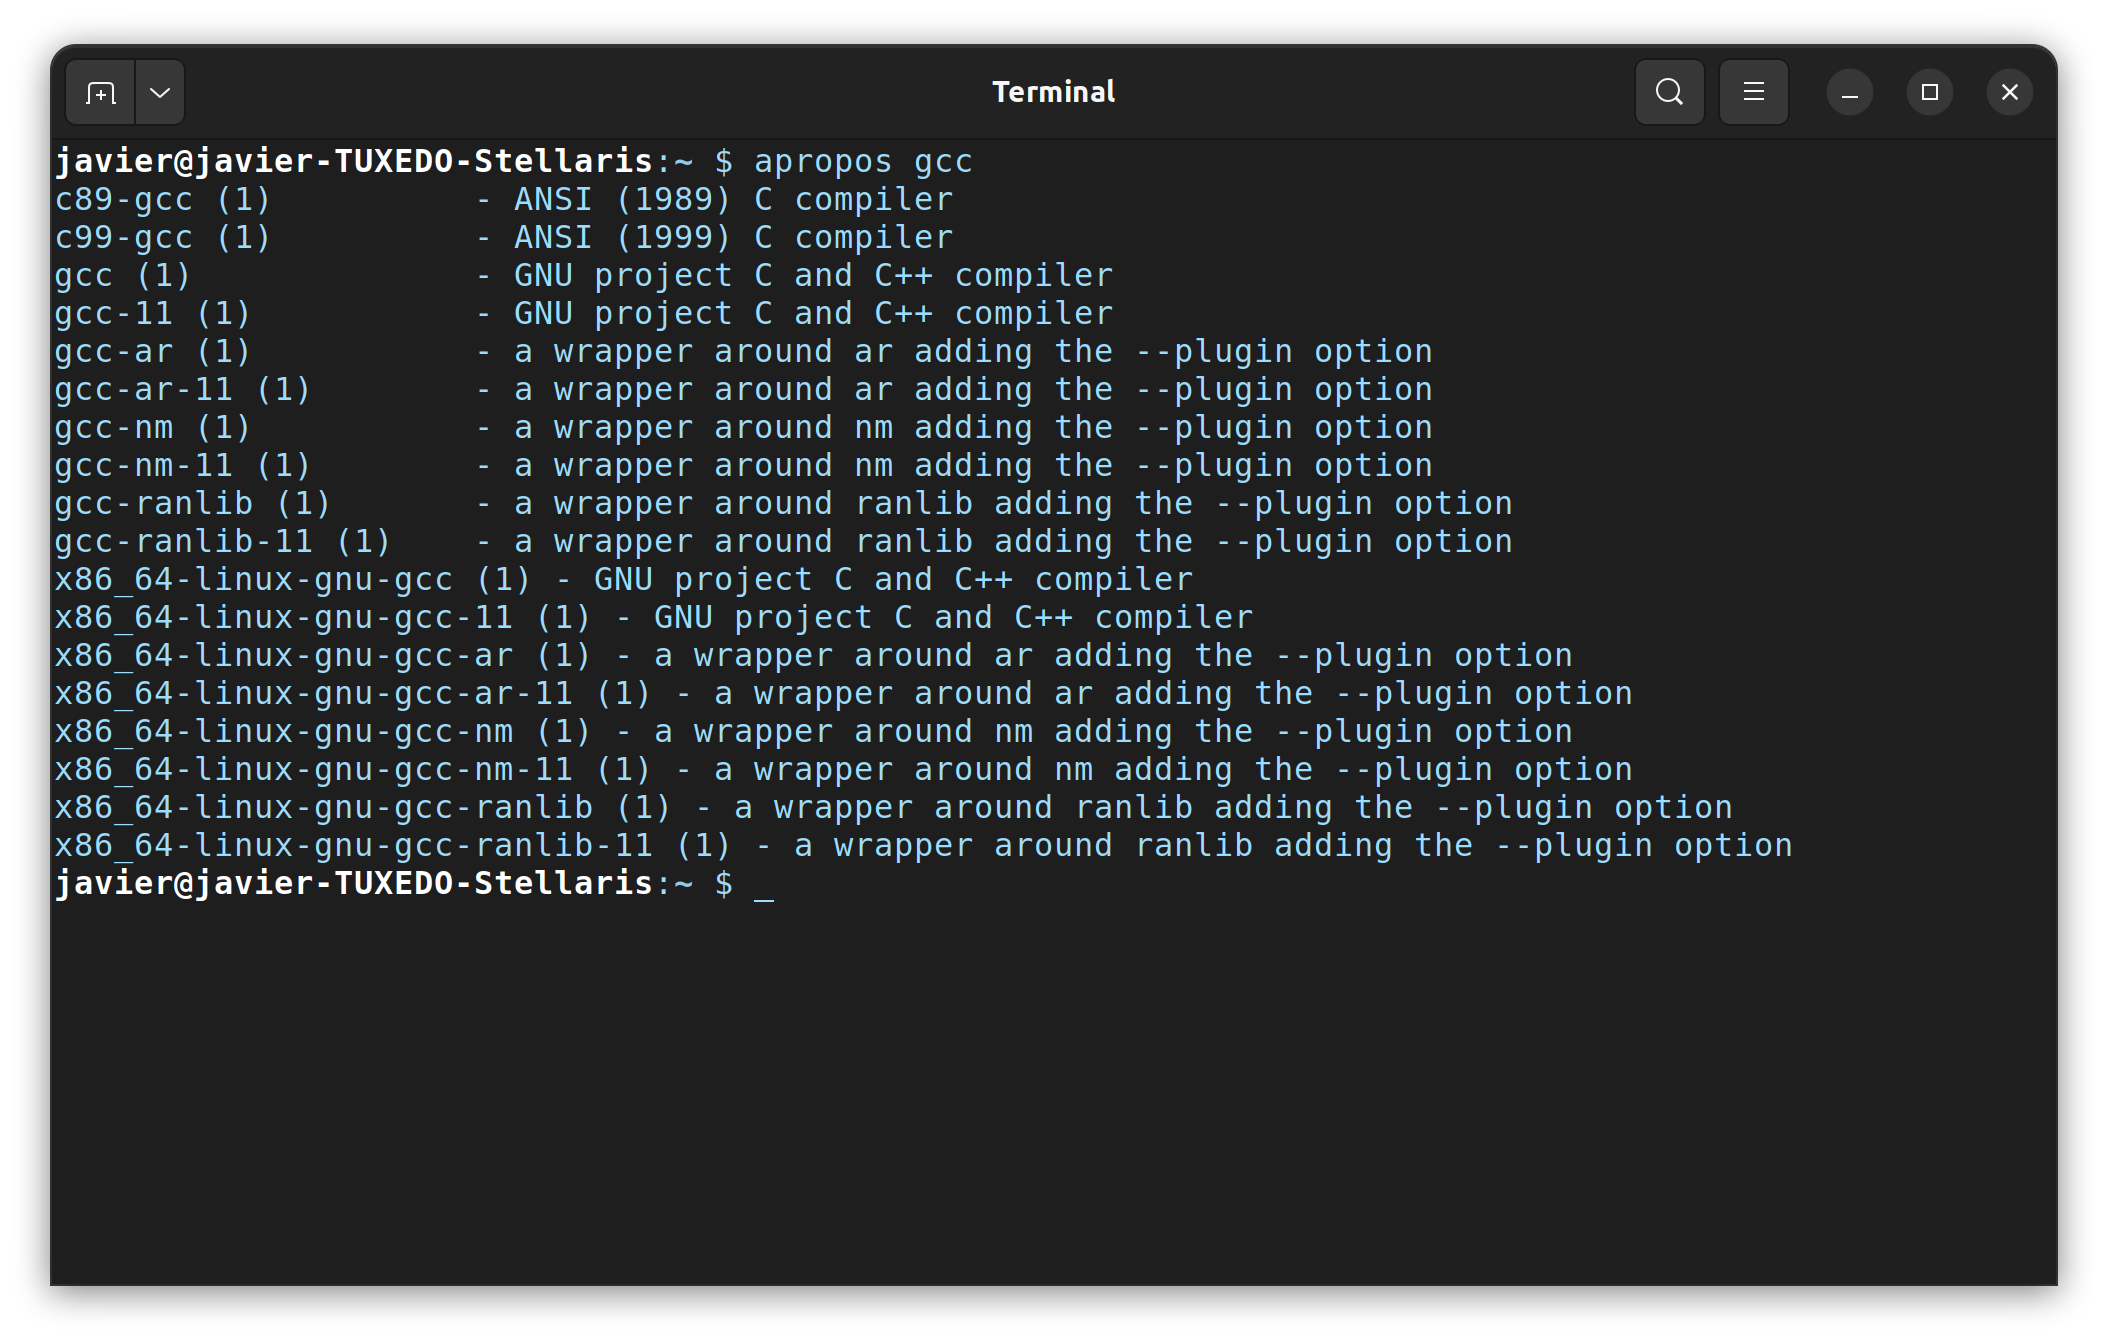
\includegraphics[width=0.55\textwidth]{apropos}
		\end{center}
	\end{frame}

	\begin{frame}
		\frametitle{Primeros comandos: date}
		\begin{alertblock}{Muestra la hora fecha actual.}
			date [OPTION]... [+FORMAT]
		\end{alertblock}
		\begin{center}
			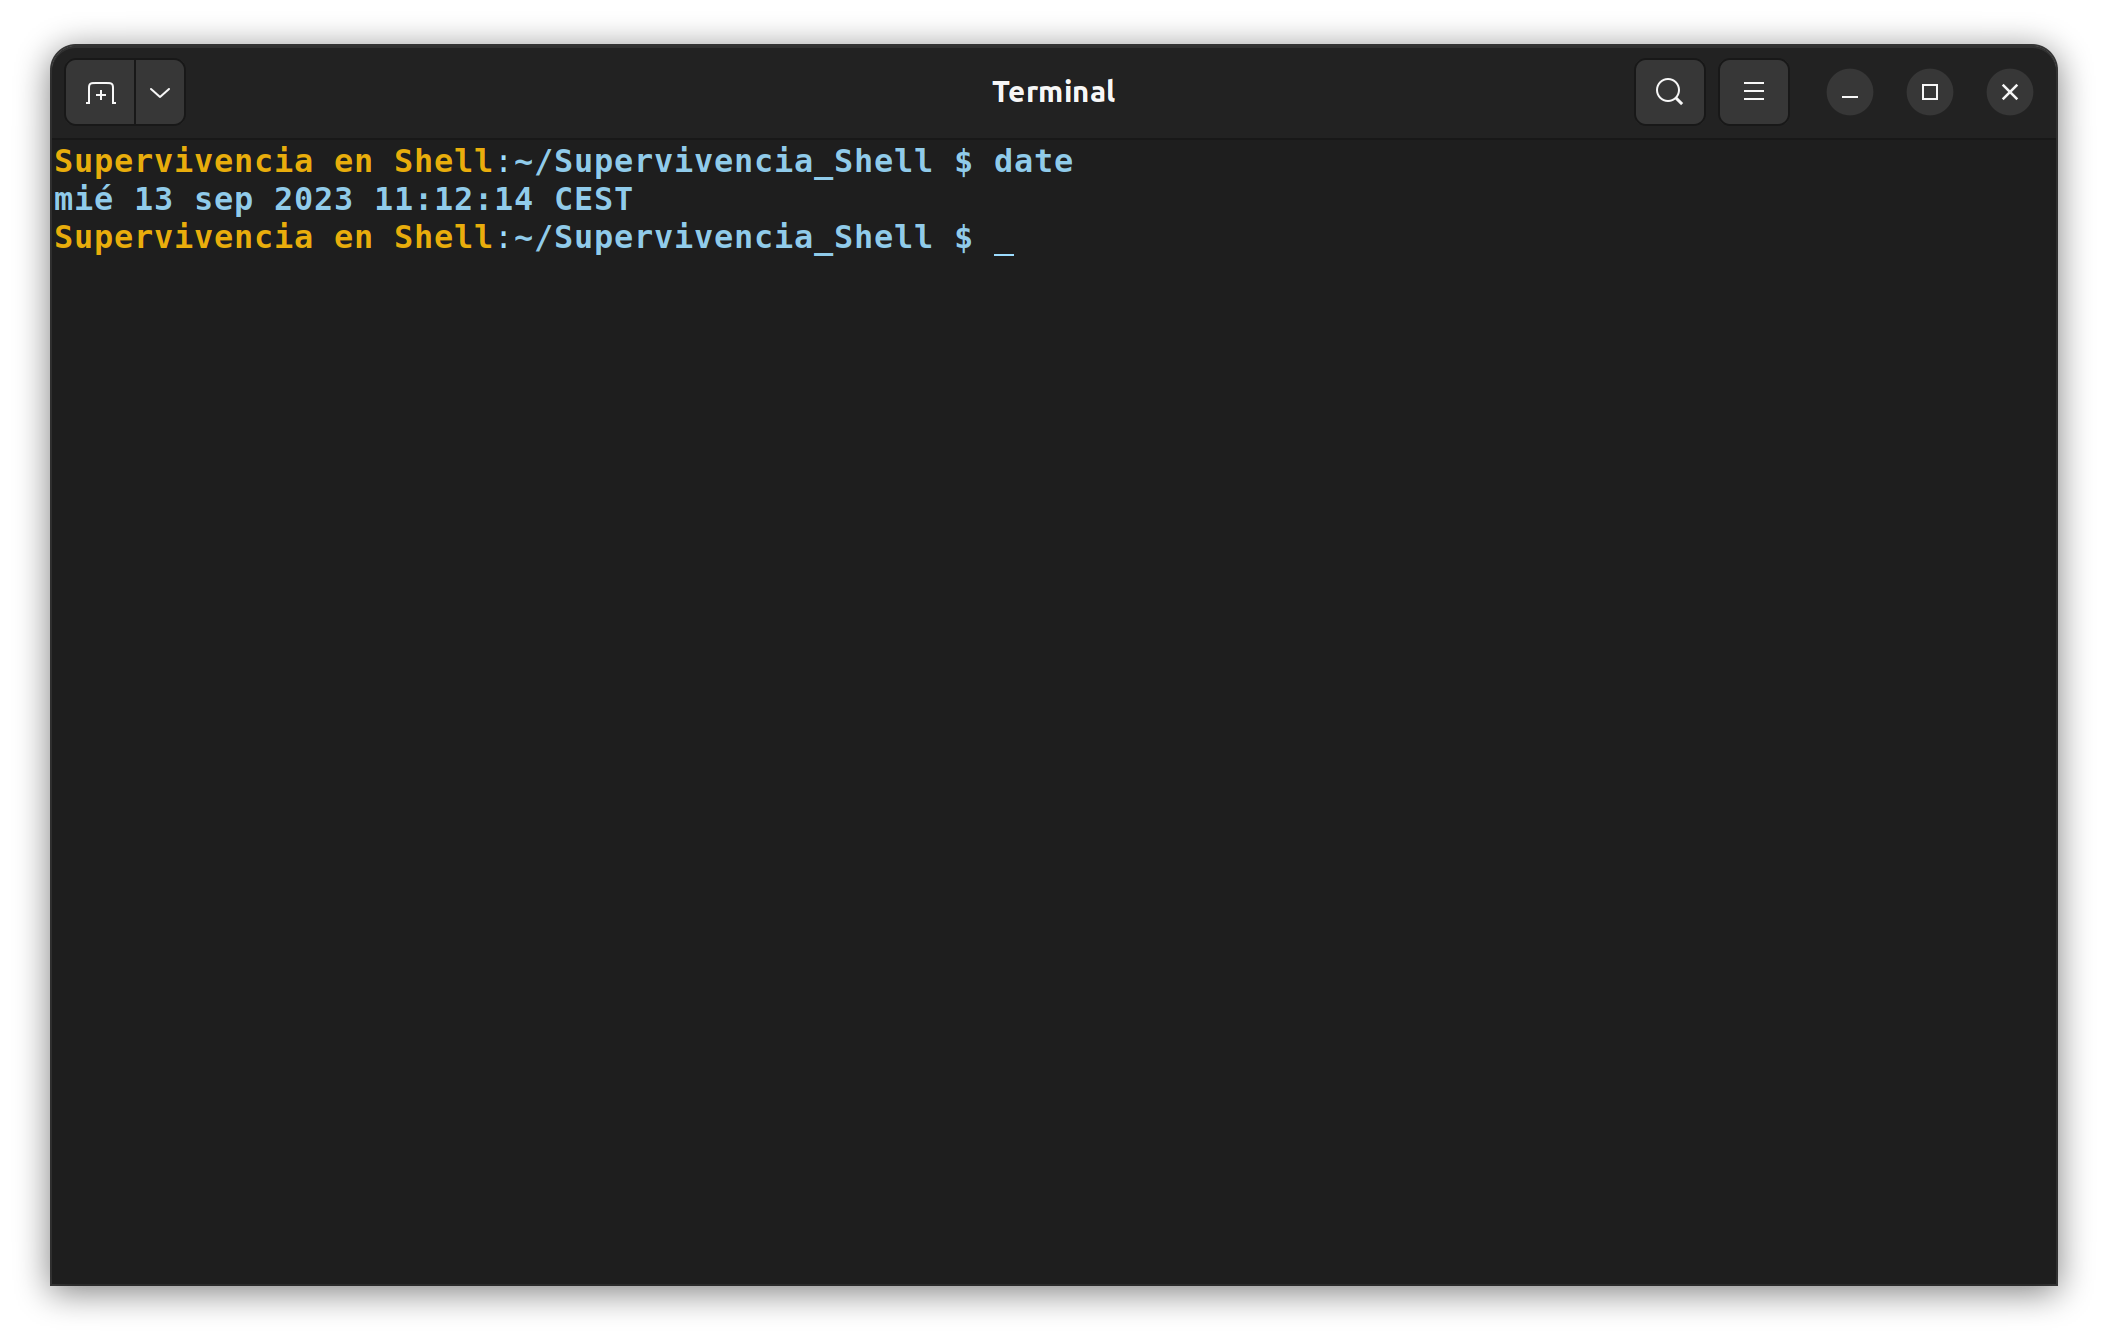
\includegraphics[width=0.55\textwidth]{date}
		\end{center}
	\end{frame}
	
	\begin{frame}
		\frametitle{Primeros comandos: who}
		\begin{alertblock}{Muestra los usuarios que están en el sistema.}
			who [OPTION]...
		\end{alertblock}
		\begin{center}
			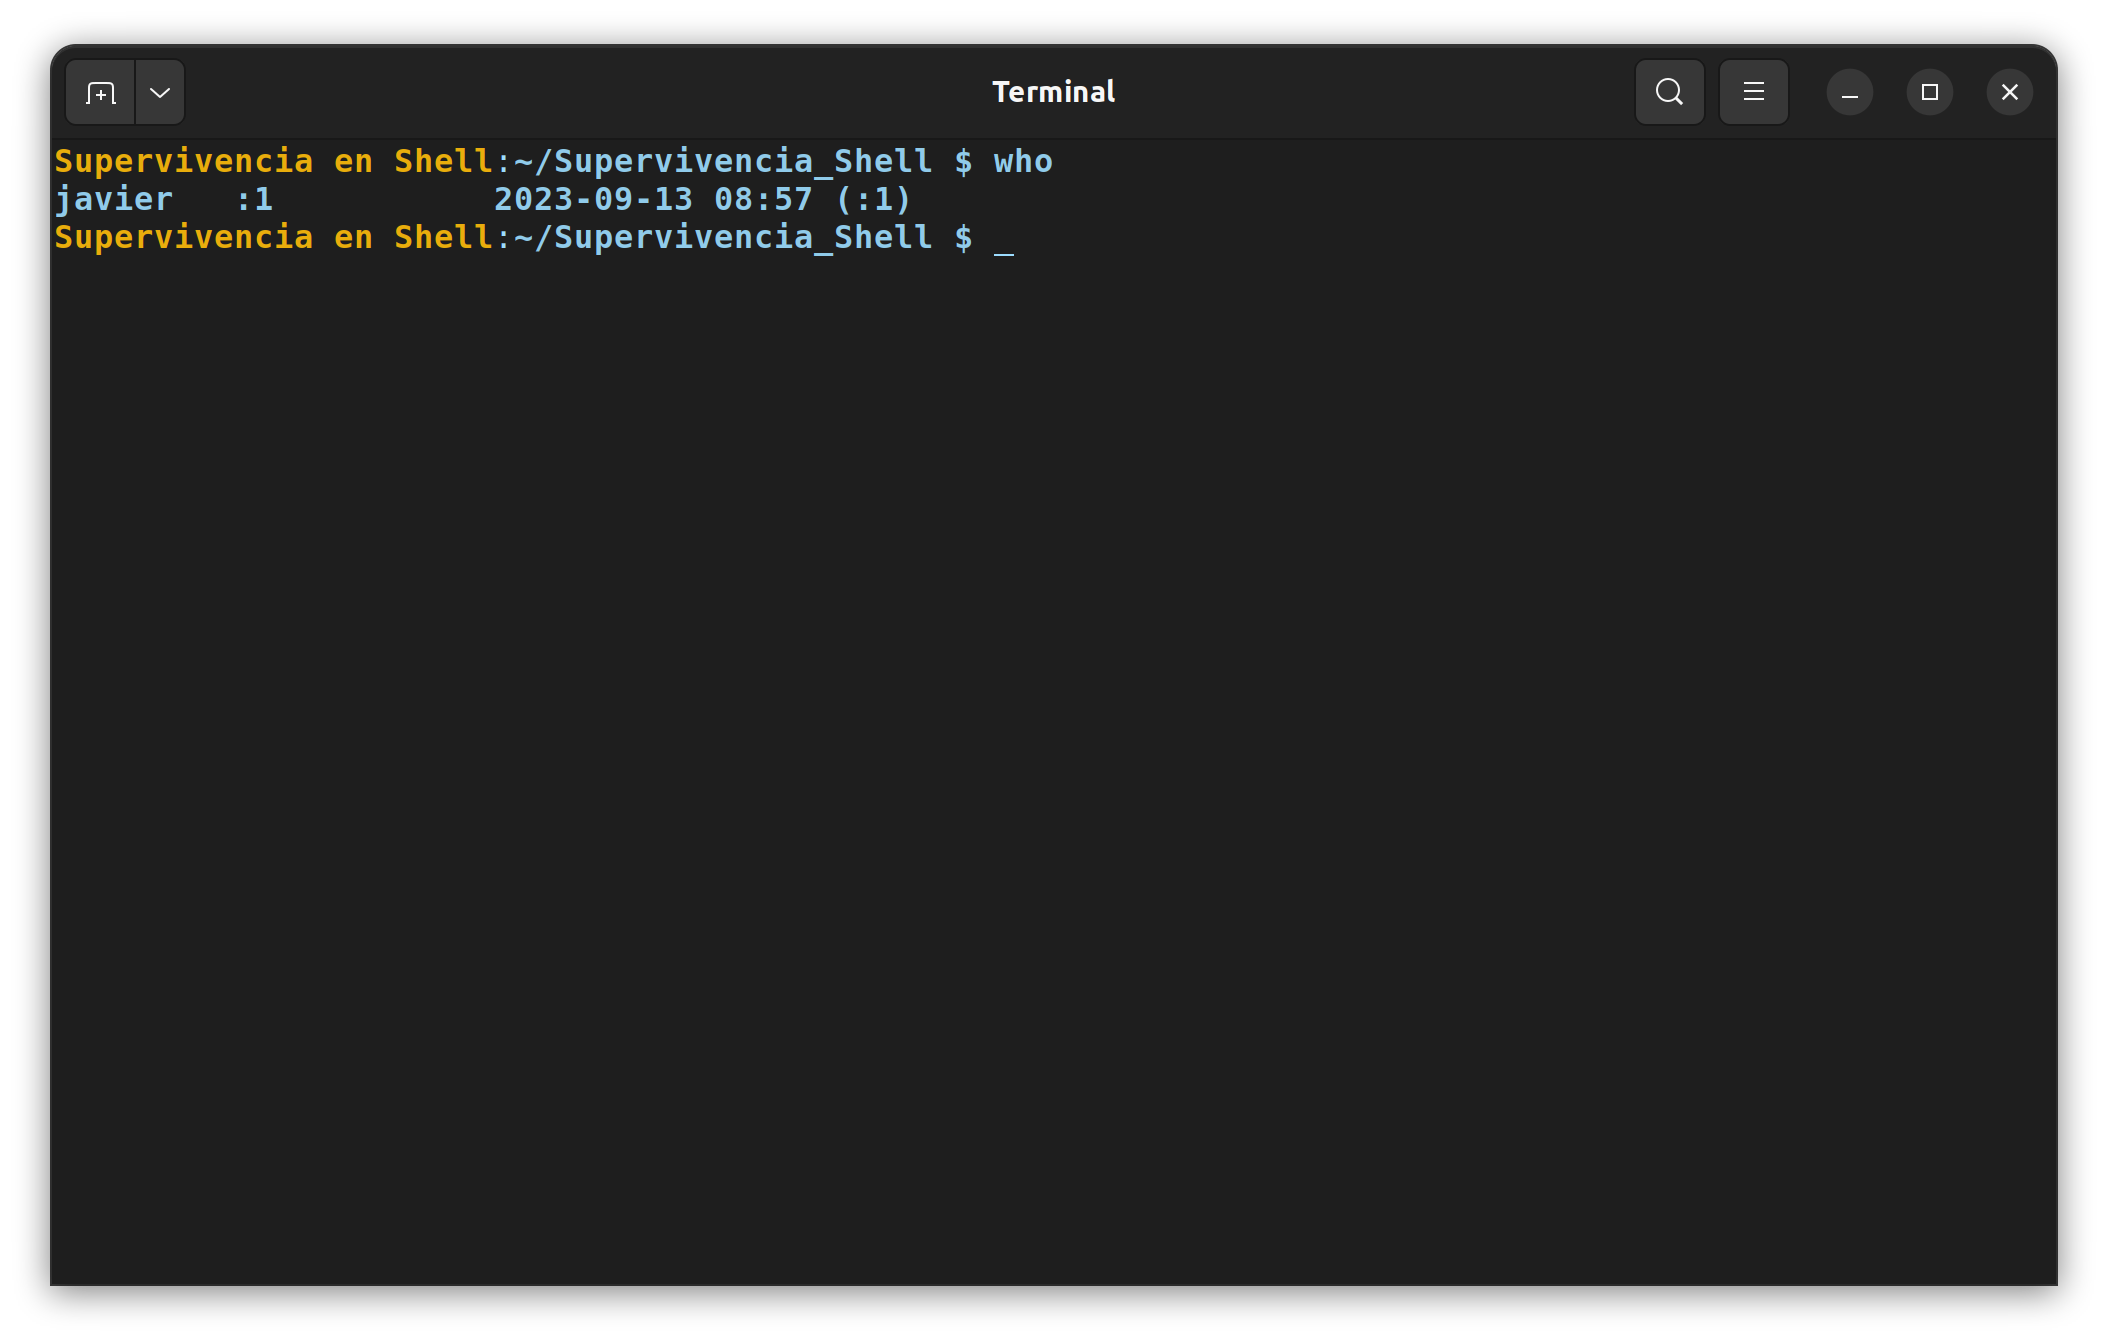
\includegraphics[width=0.55\textwidth]{who}
		\end{center}
	\end{frame}
	
	\begin{frame}
		\frametitle{Primeros comandos: whoami}
		\begin{alertblock}{Muestra tu nombre de usuario.}
			whoami [OPTION]...
		\end{alertblock}
		\begin{center}
			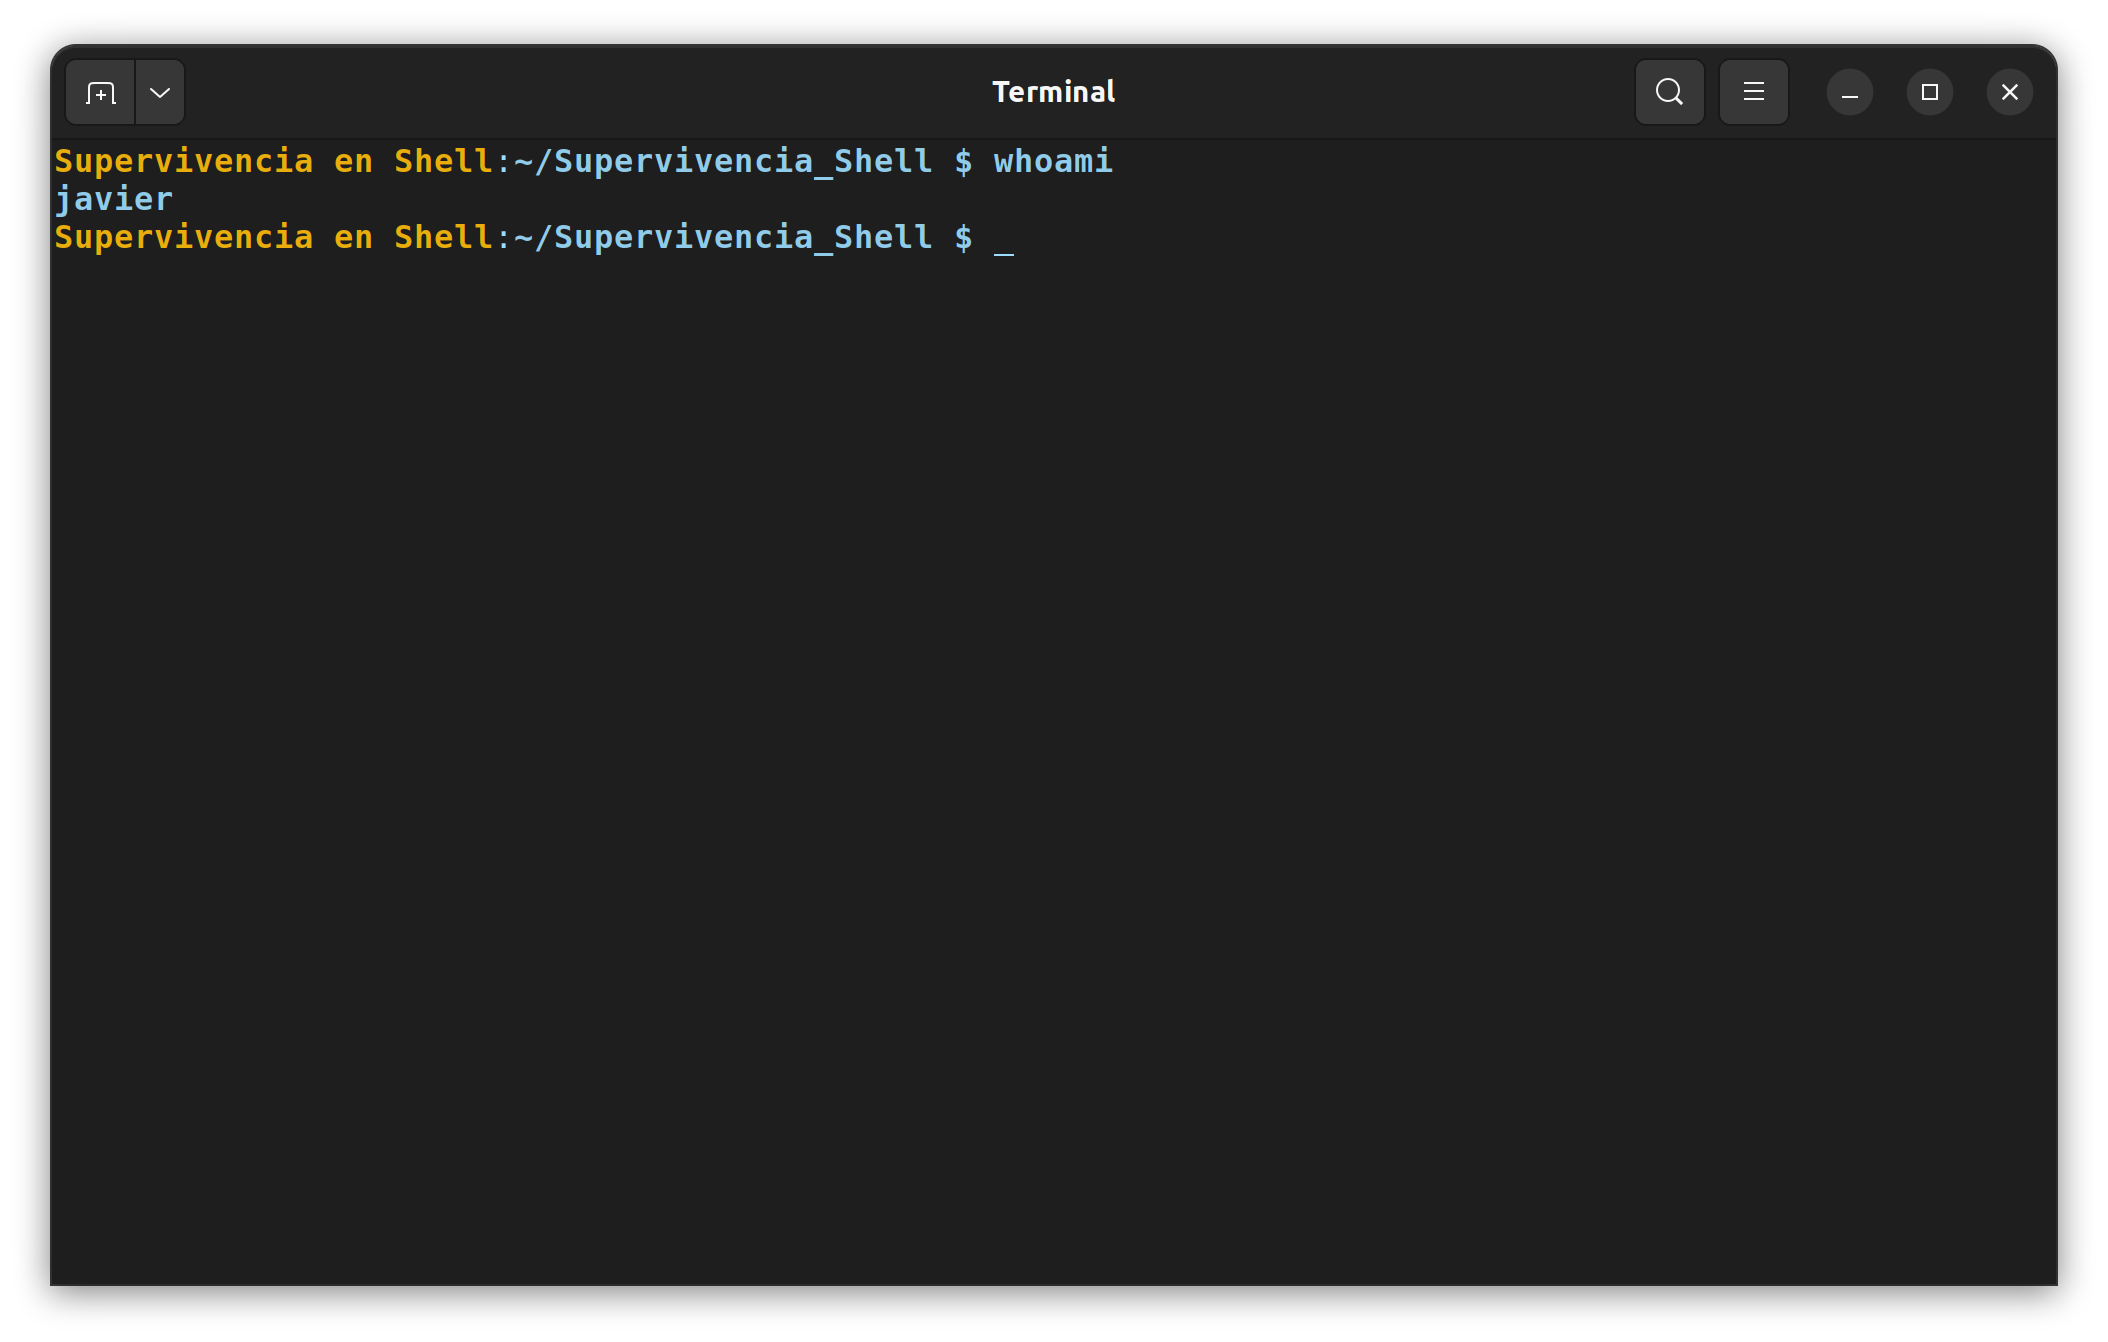
\includegraphics[width=0.55\textwidth]{whoami}
		\end{center}
	\end{frame}
	
	\begin{frame}
		\frametitle{Primeros compandos: echo}
		\begin{alertblock}{Escribe sus argumentos por su salida.}
			echo [SHORT-OPTION]... [STRING]...
		\end{alertblock}
		\begin{center}
			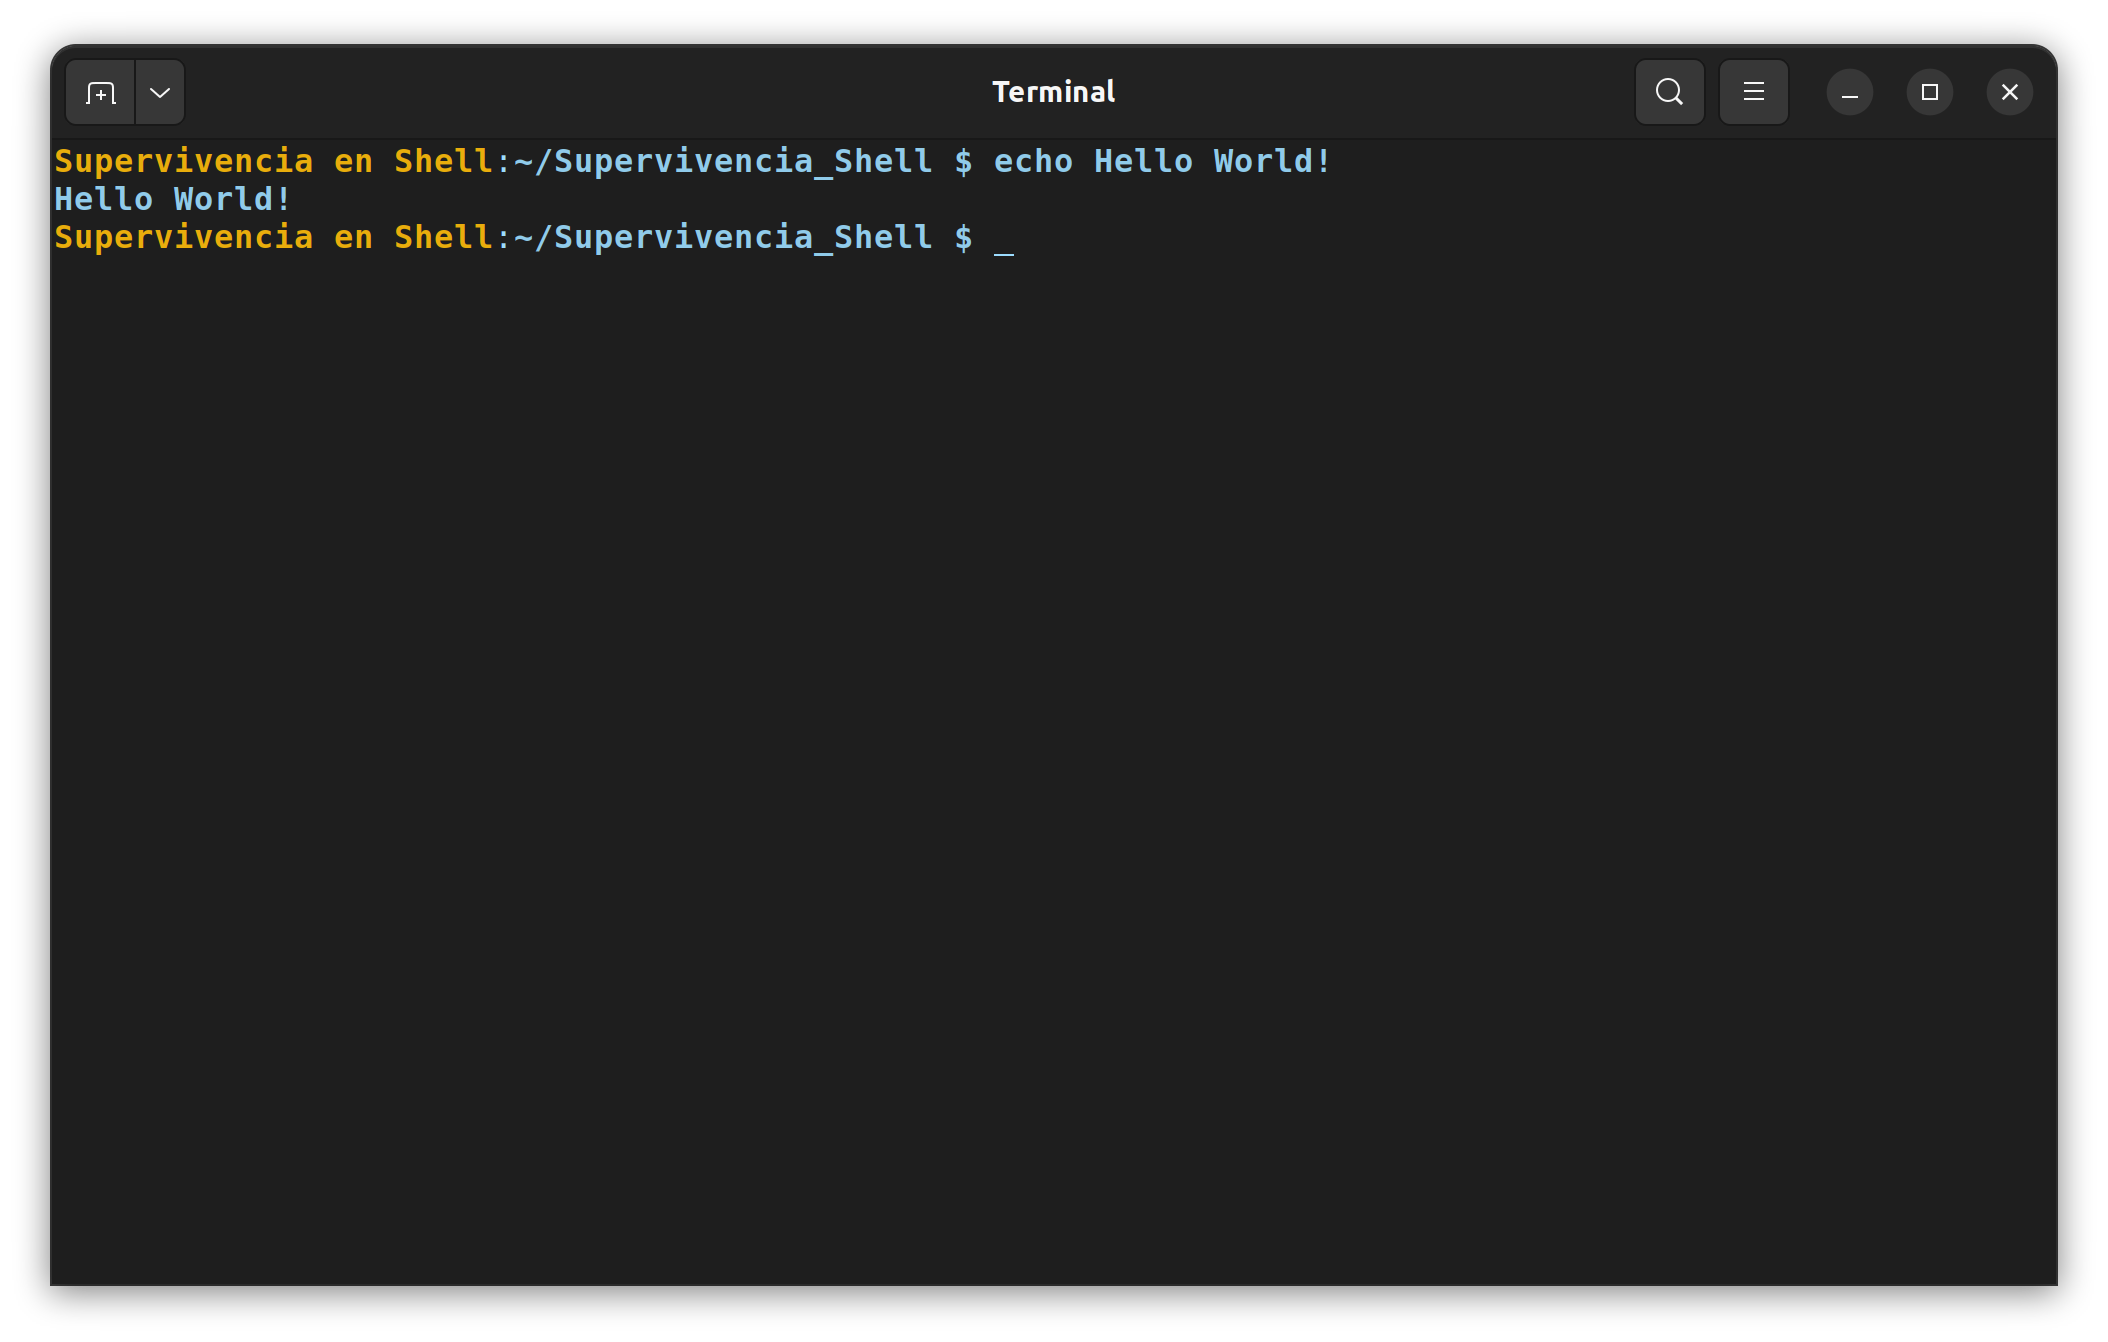
\includegraphics[width=0.55\textwidth]{echo}
		\end{center}
	\end{frame}
	
	\begin{frame}
		\frametitle{Navegando por el terminal: Tabulador}
		\begin{alertblock}{El tabulador es tu amigo, no dudes en usarlo.}
			Autocompleta el argumento y en caso de varios resultados muestra una lista
		\end{alertblock}
		\begin{center}
			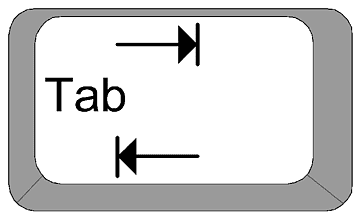
\includegraphics[width=0.35\textwidth]{tab}
		\end{center}
	\end{frame}
	
	\begin{frame}
		\frametitle{Navegando por el terminal: Historial}
		\begin{alertblock}{Se navega por el historial usando las flechas.}
			Flecha hacia arriba muestra el comando anterior.\\
			Flecha hacia abajo muestra el comando siguiente.\\
			También se puede buscar usando Ctr + R.
		\end{alertblock}
		\begin{center}
			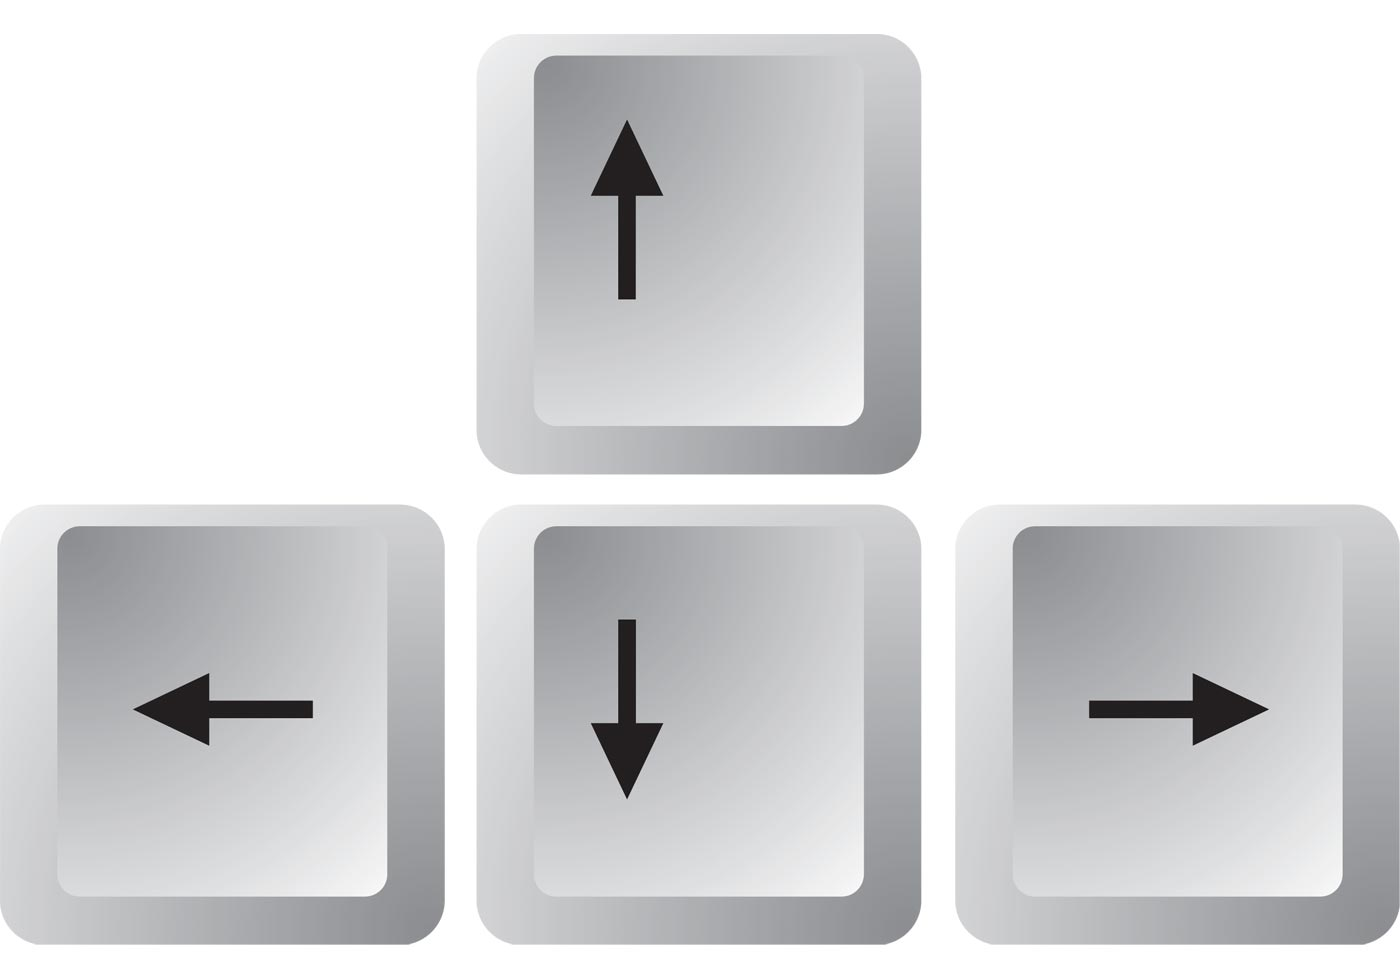
\includegraphics[width=0.35\textwidth]{keys}
		\end{center}
	\end{frame}
	
	\begin{frame}
		\frametitle{Navegando por el terminal: ls}
		\begin{alertblock}{Lista el contenido de un directorio.}
			ls [OPTION]...
		\end{alertblock}
		\begin{center}
			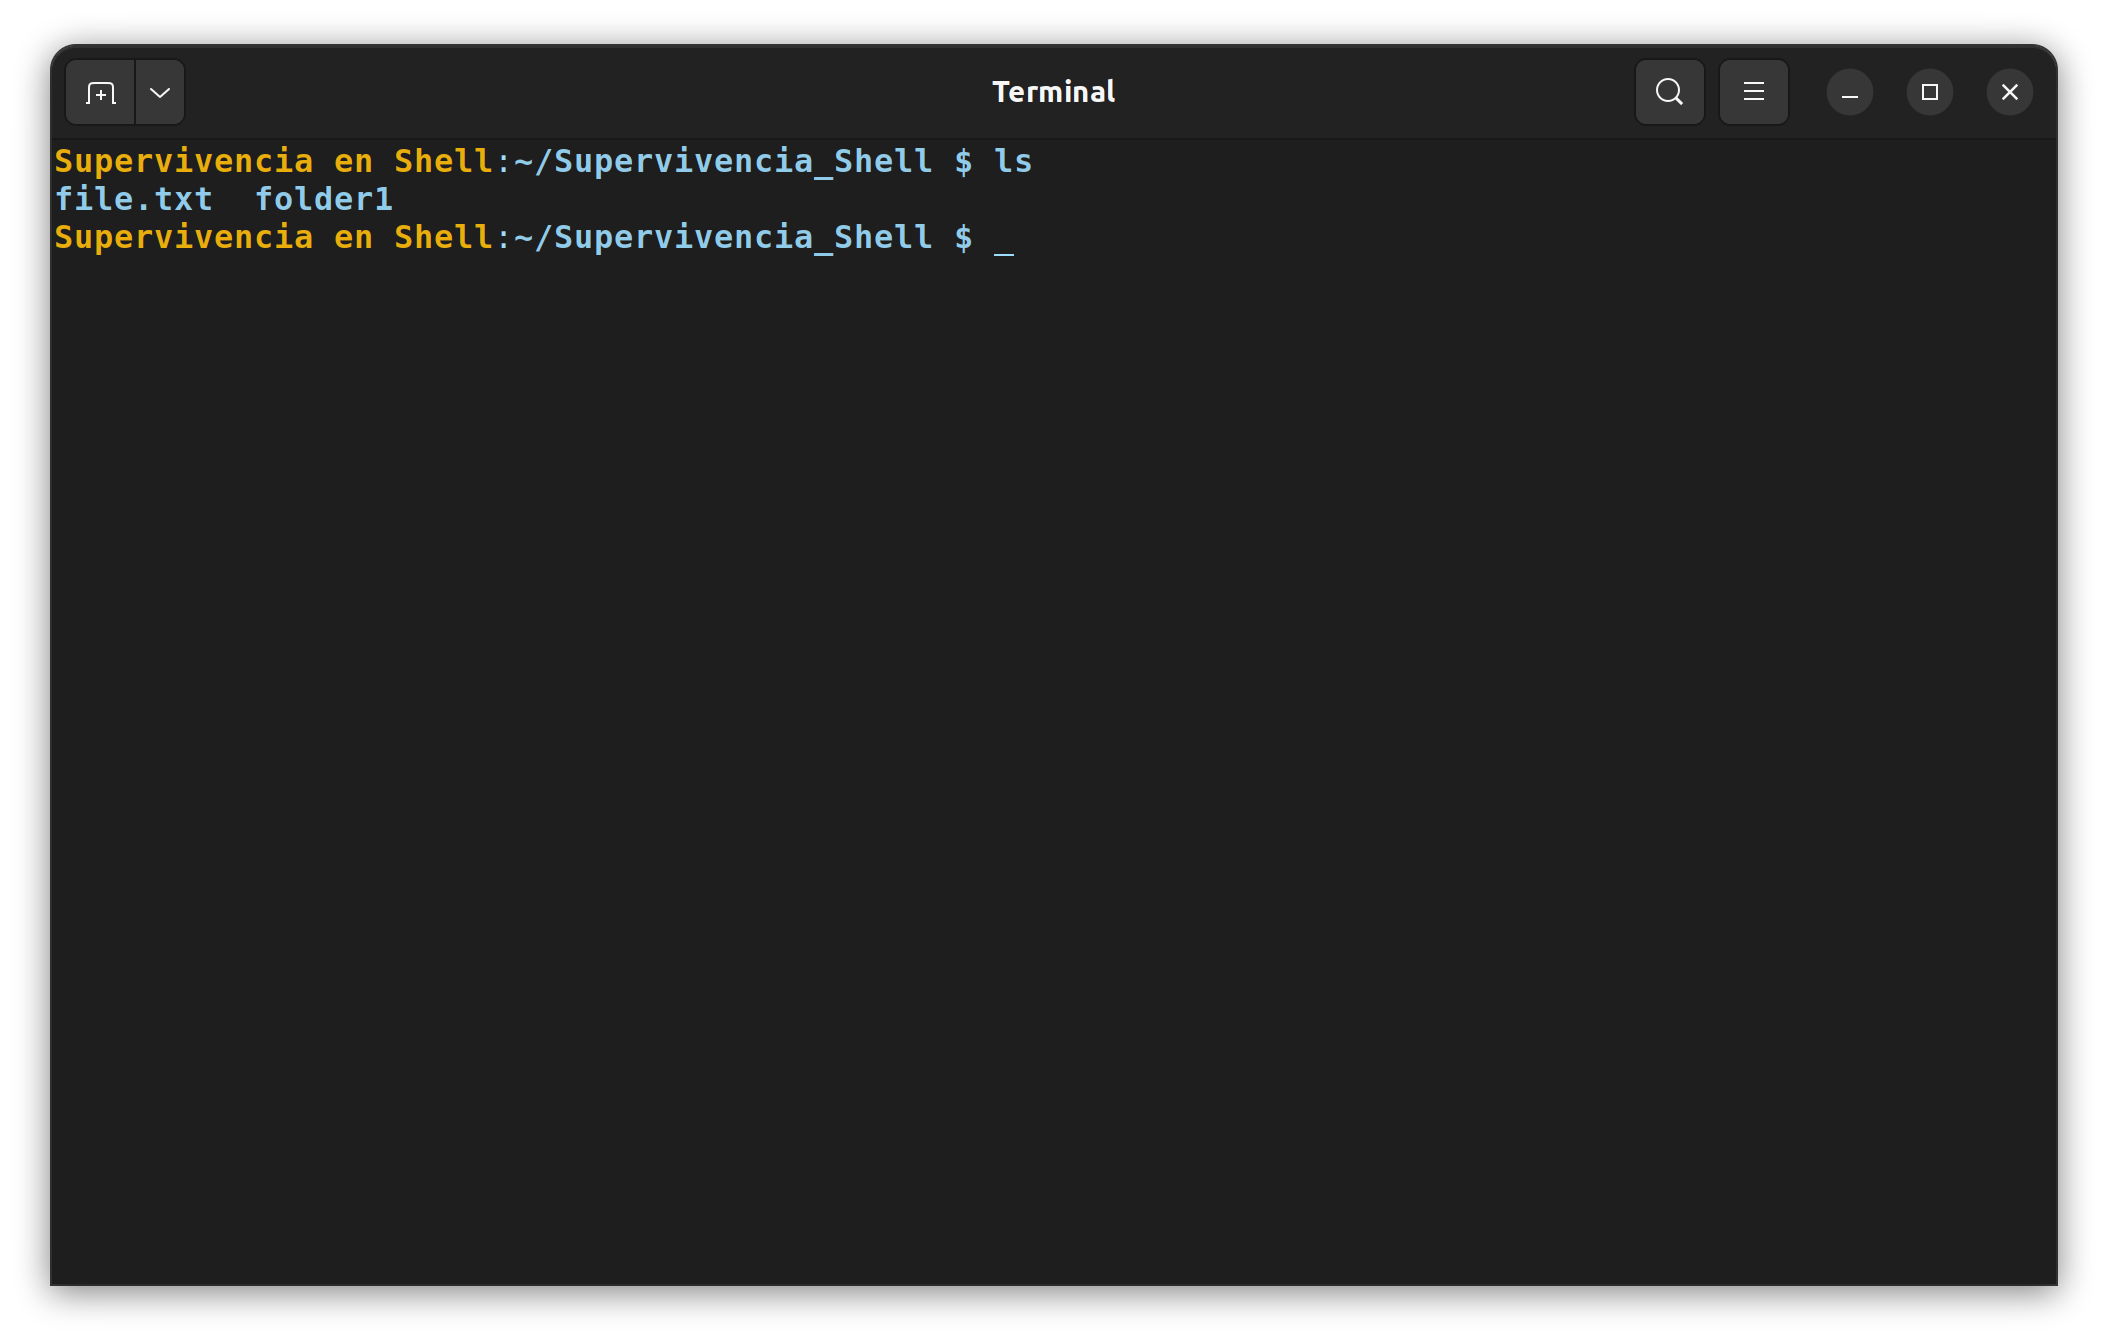
\includegraphics[width=0.55\textwidth]{ls}
		\end{center}
	\end{frame}
	
	\begin{frame}
		\frametitle{Navegando por el terminal: cd}
		\begin{alertblock}{Cambia de directorio actual.}
			cd [dir]
		\end{alertblock}
		\begin{center}
			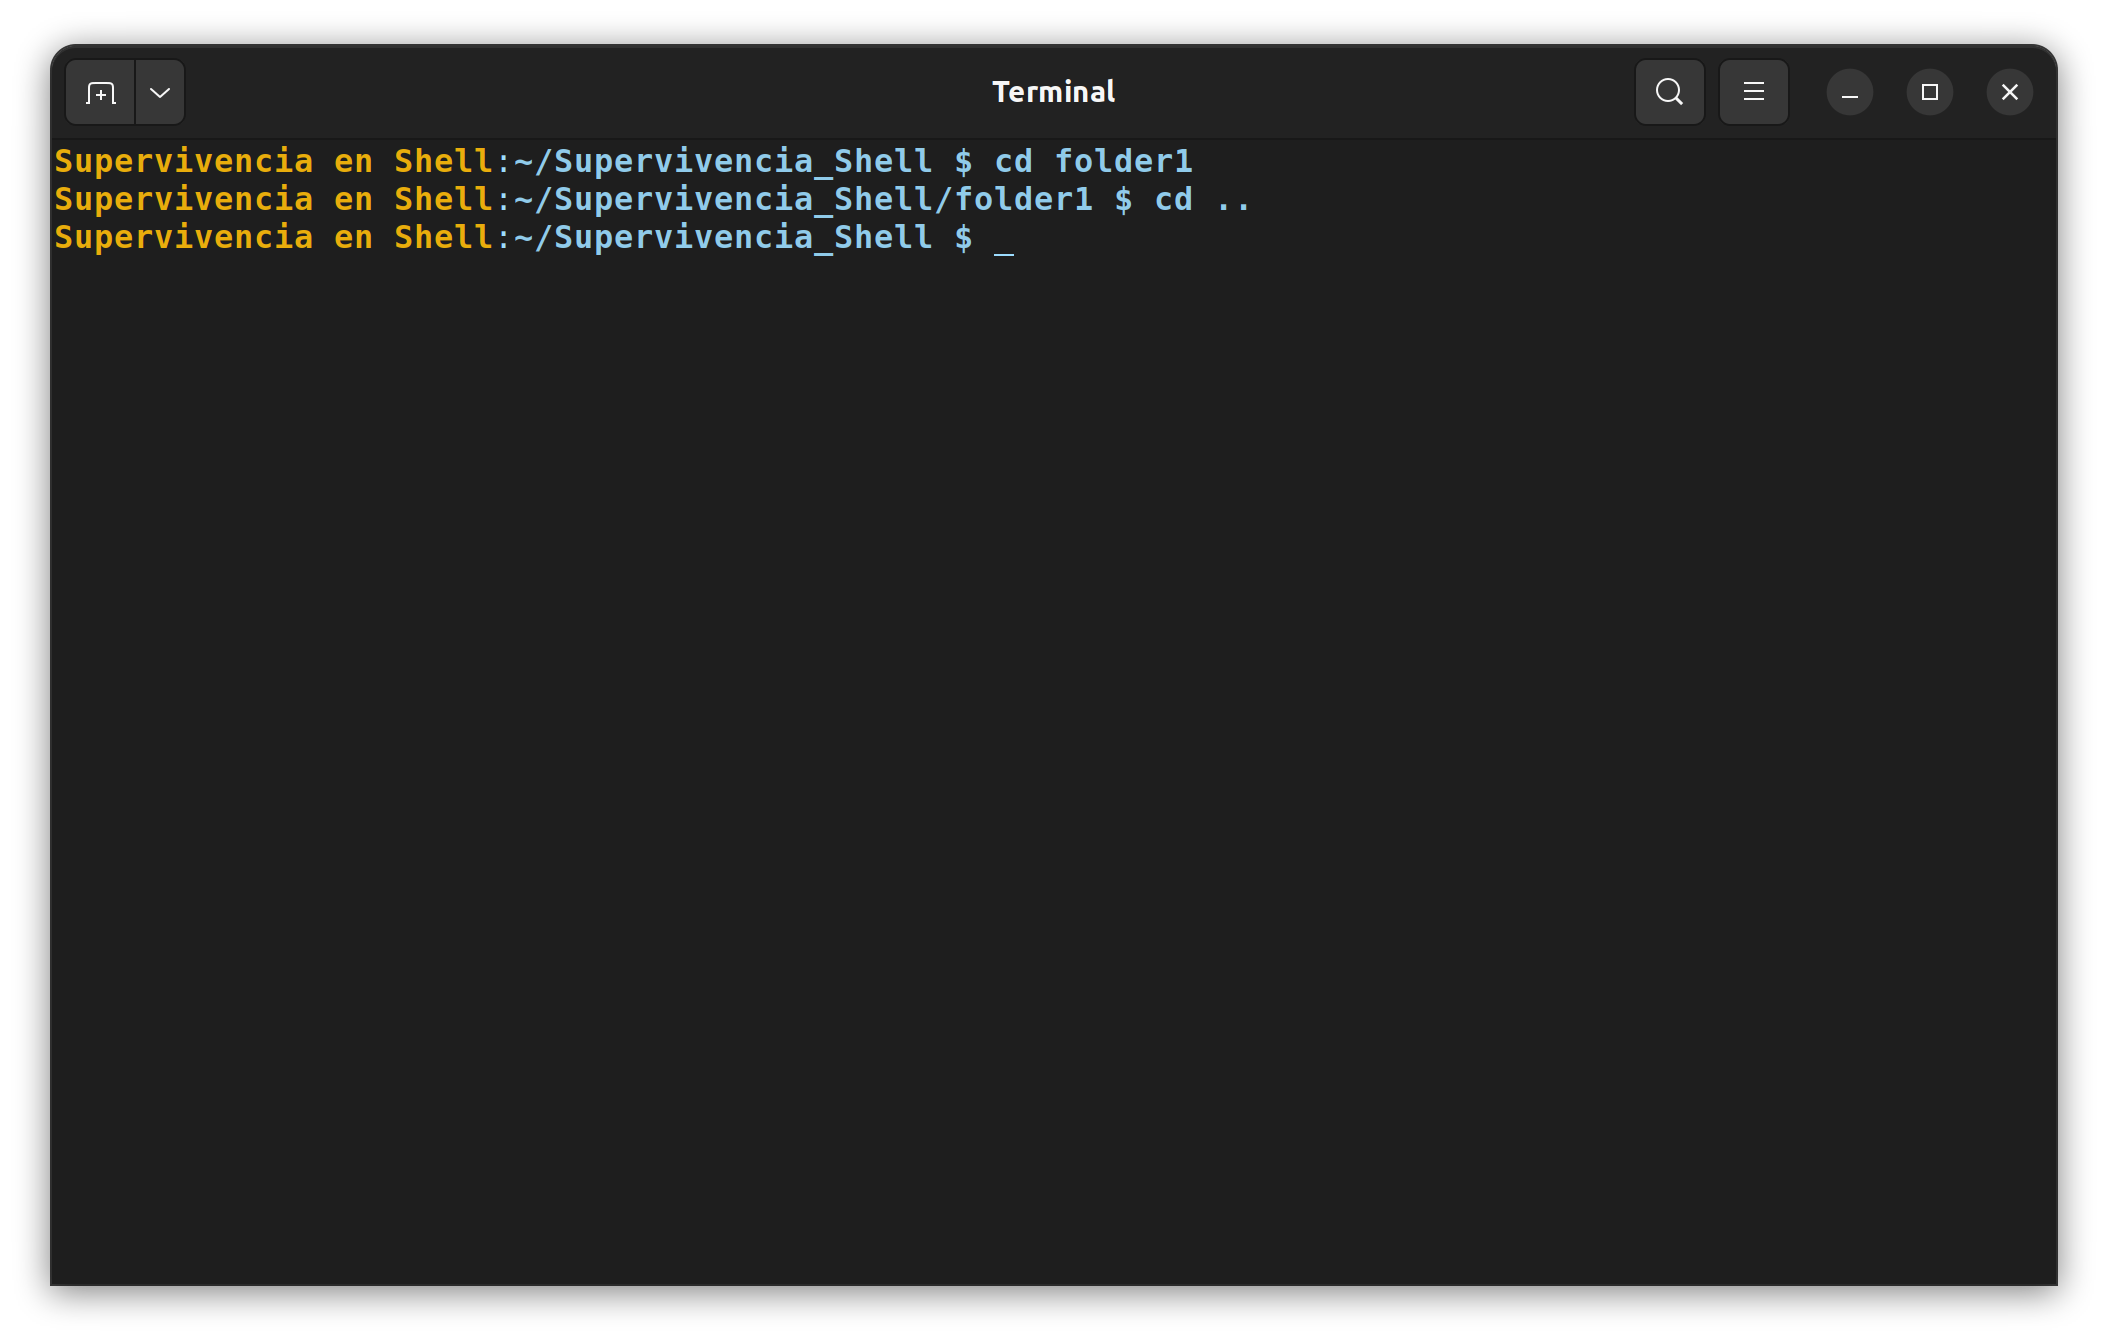
\includegraphics[width=0.55\textwidth]{cd}
		\end{center}
	\end{frame}
	
	\begin{frame}
		\frametitle{Navegando por el terminal: touch}
		\begin{alertblock}{Cambia la fecha de modificación de un fichero, y si no existe, se crea.}
			touch [OPTION]... FILE...
		\end{alertblock}
		\begin{center}
			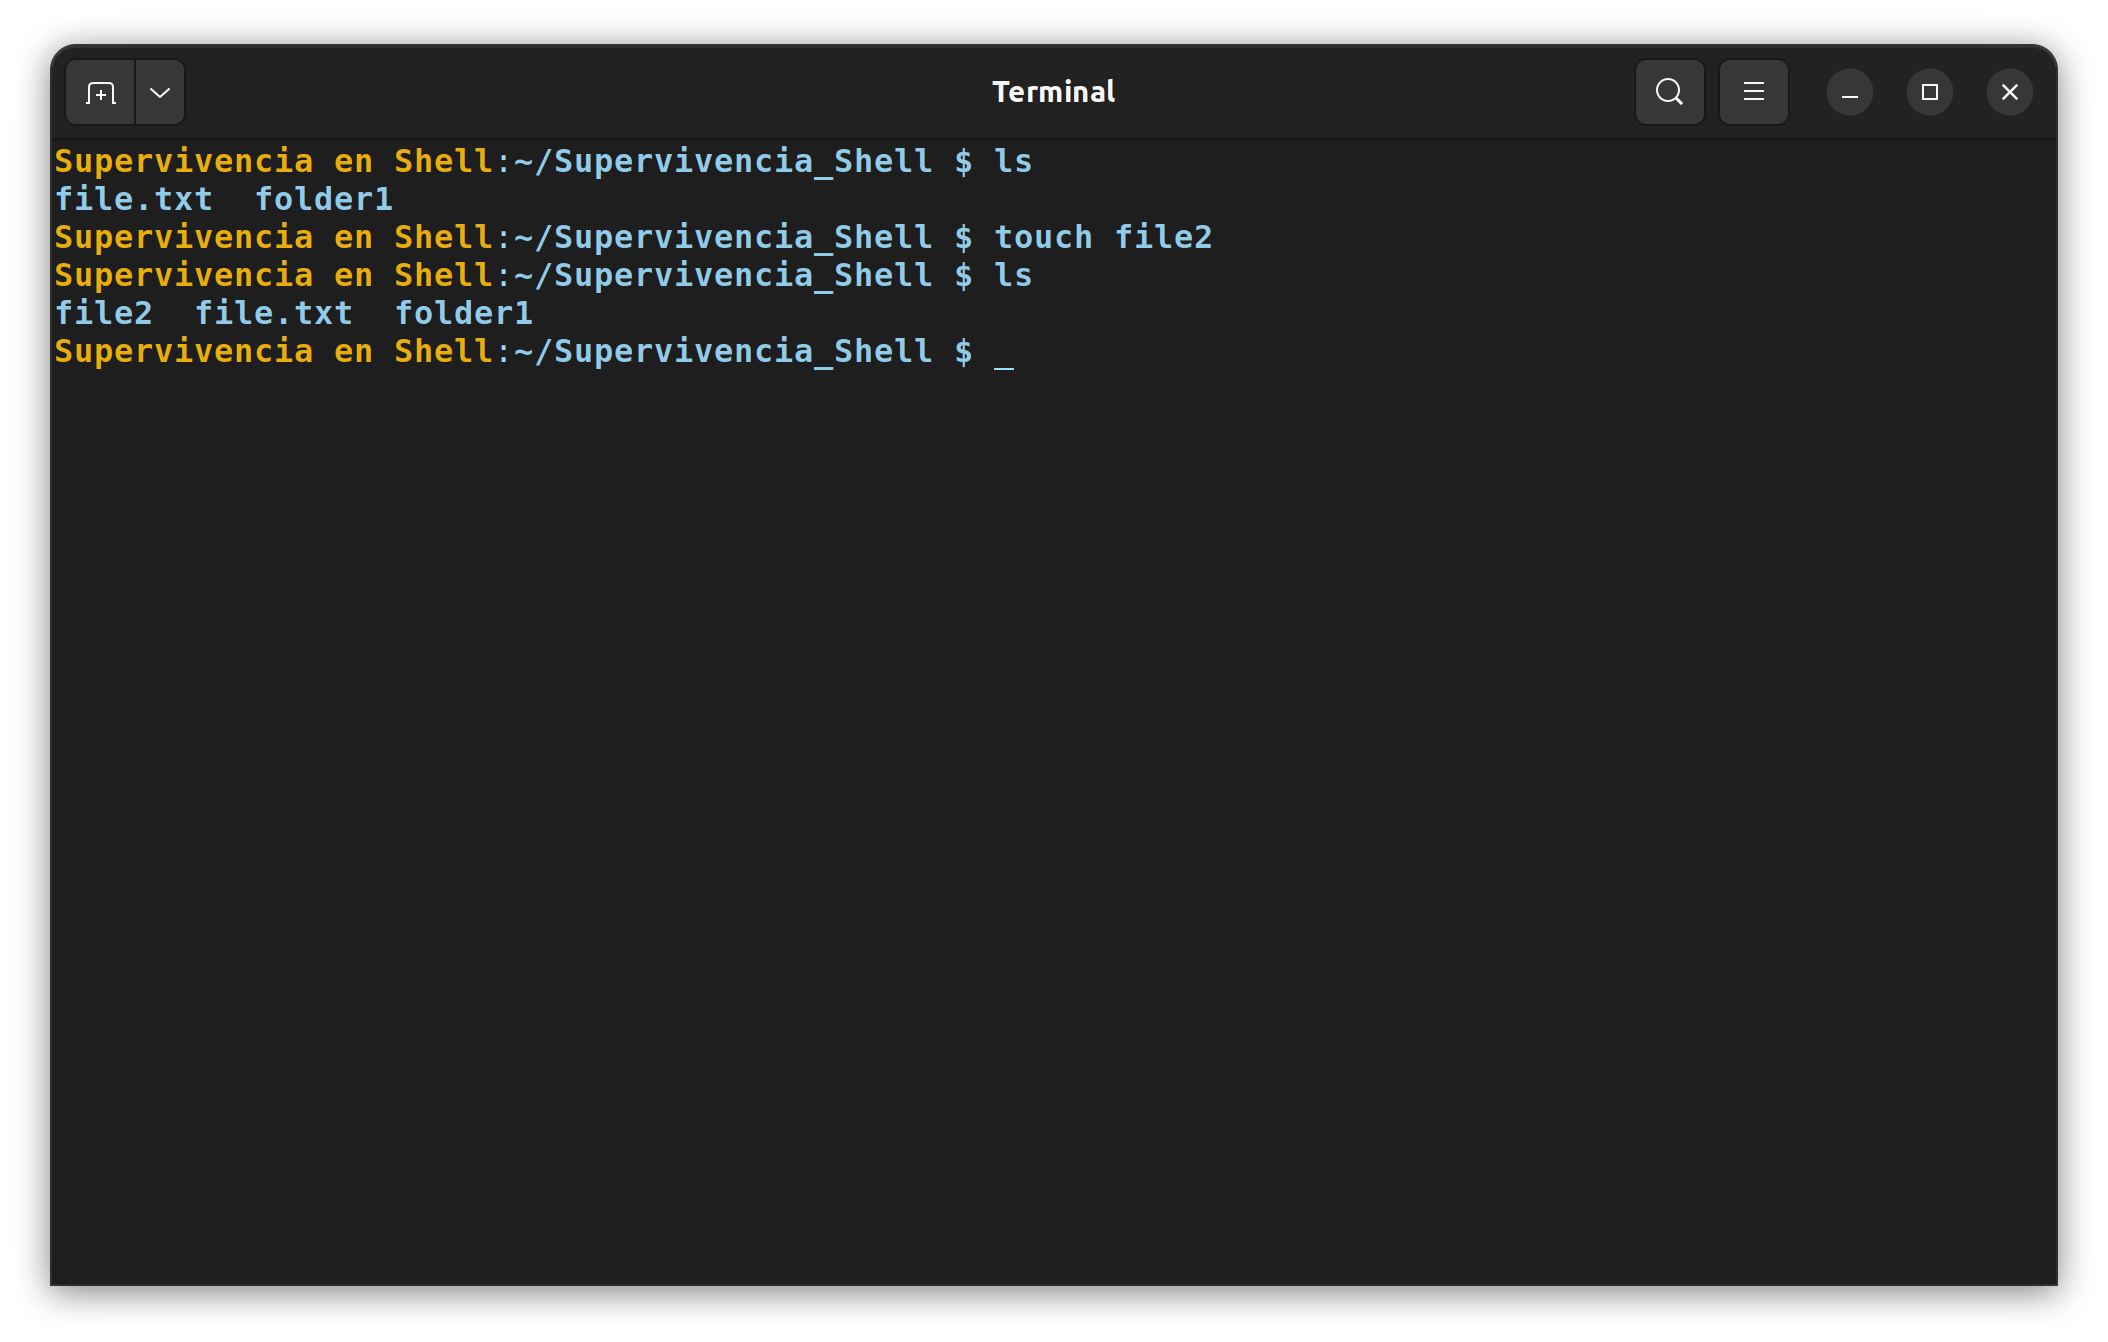
\includegraphics[width=0.55\textwidth]{touch}
		\end{center}
	\end{frame}
	
	\begin{frame}
		\frametitle{Navegando por el terminal: cp}
		\begin{alertblock}{Copia ficheros.}
			cp [OPTION]... SOURCE DEST
		\end{alertblock}
		\begin{center}
			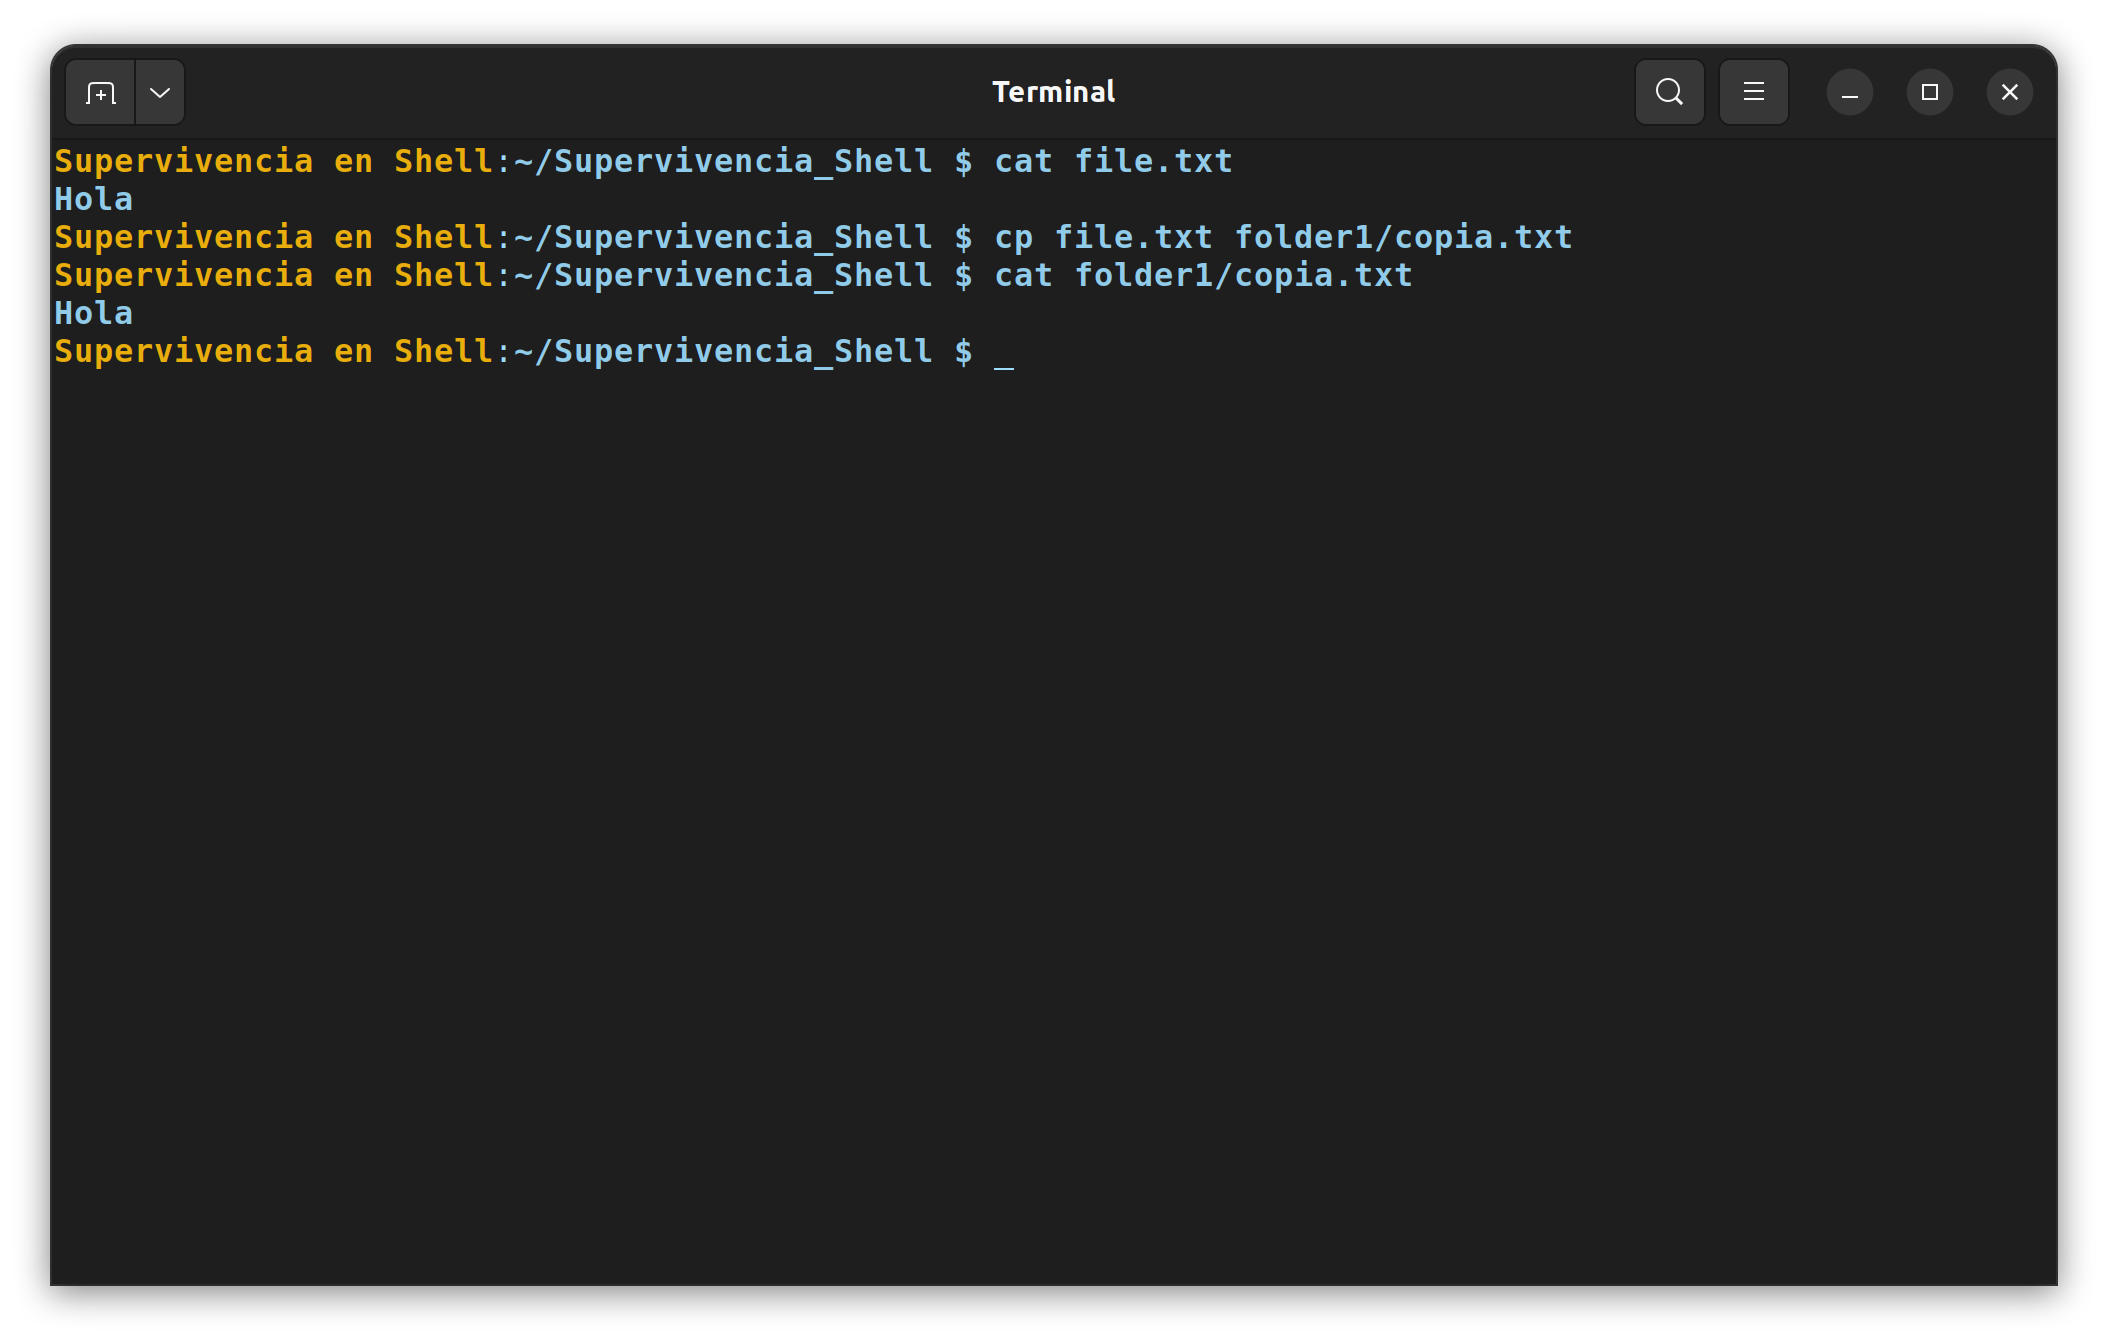
\includegraphics[width=0.55\textwidth]{cp}
		\end{center}
	\end{frame}	
		
	\begin{frame}
		\frametitle{Navegando por el terminal: mv}
		\begin{alertblock}{Mueve fichheros.}
			mv [OPTION]... SOURCE DEST
		\end{alertblock}
		\begin{center}
			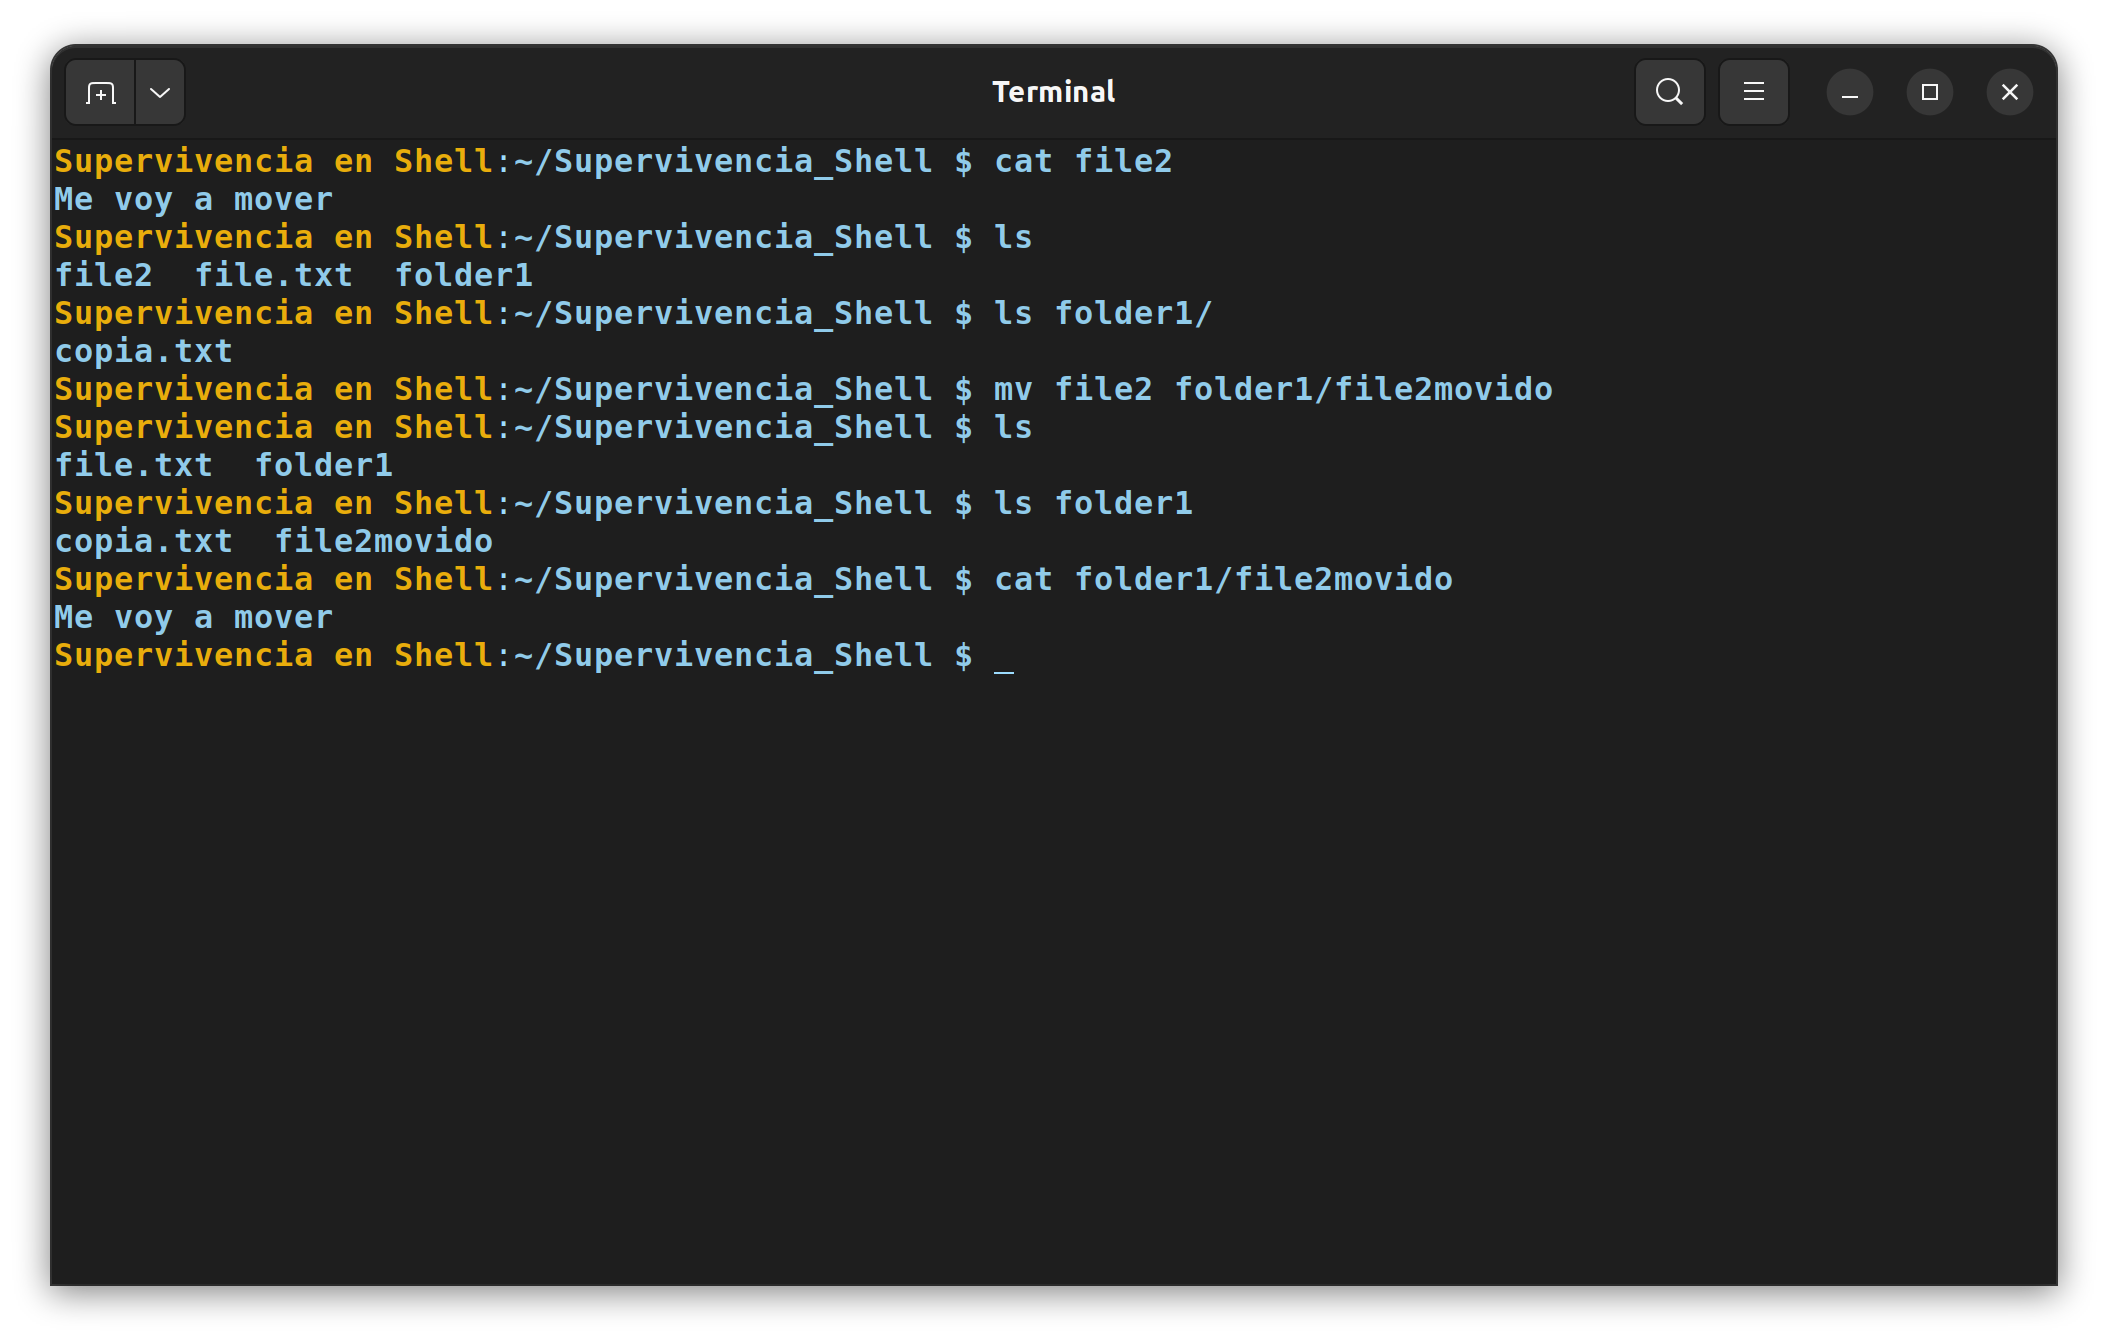
\includegraphics[width=0.55\textwidth]{mv}
		\end{center}
	\end{frame}	
		
	\begin{frame}
		\frametitle{Navegando por el terminal: rm}
		\begin{alertblock}{Borra ficheros.}
			rm [OPTION]... [FILE]...
		\end{alertblock}
		\begin{center}
			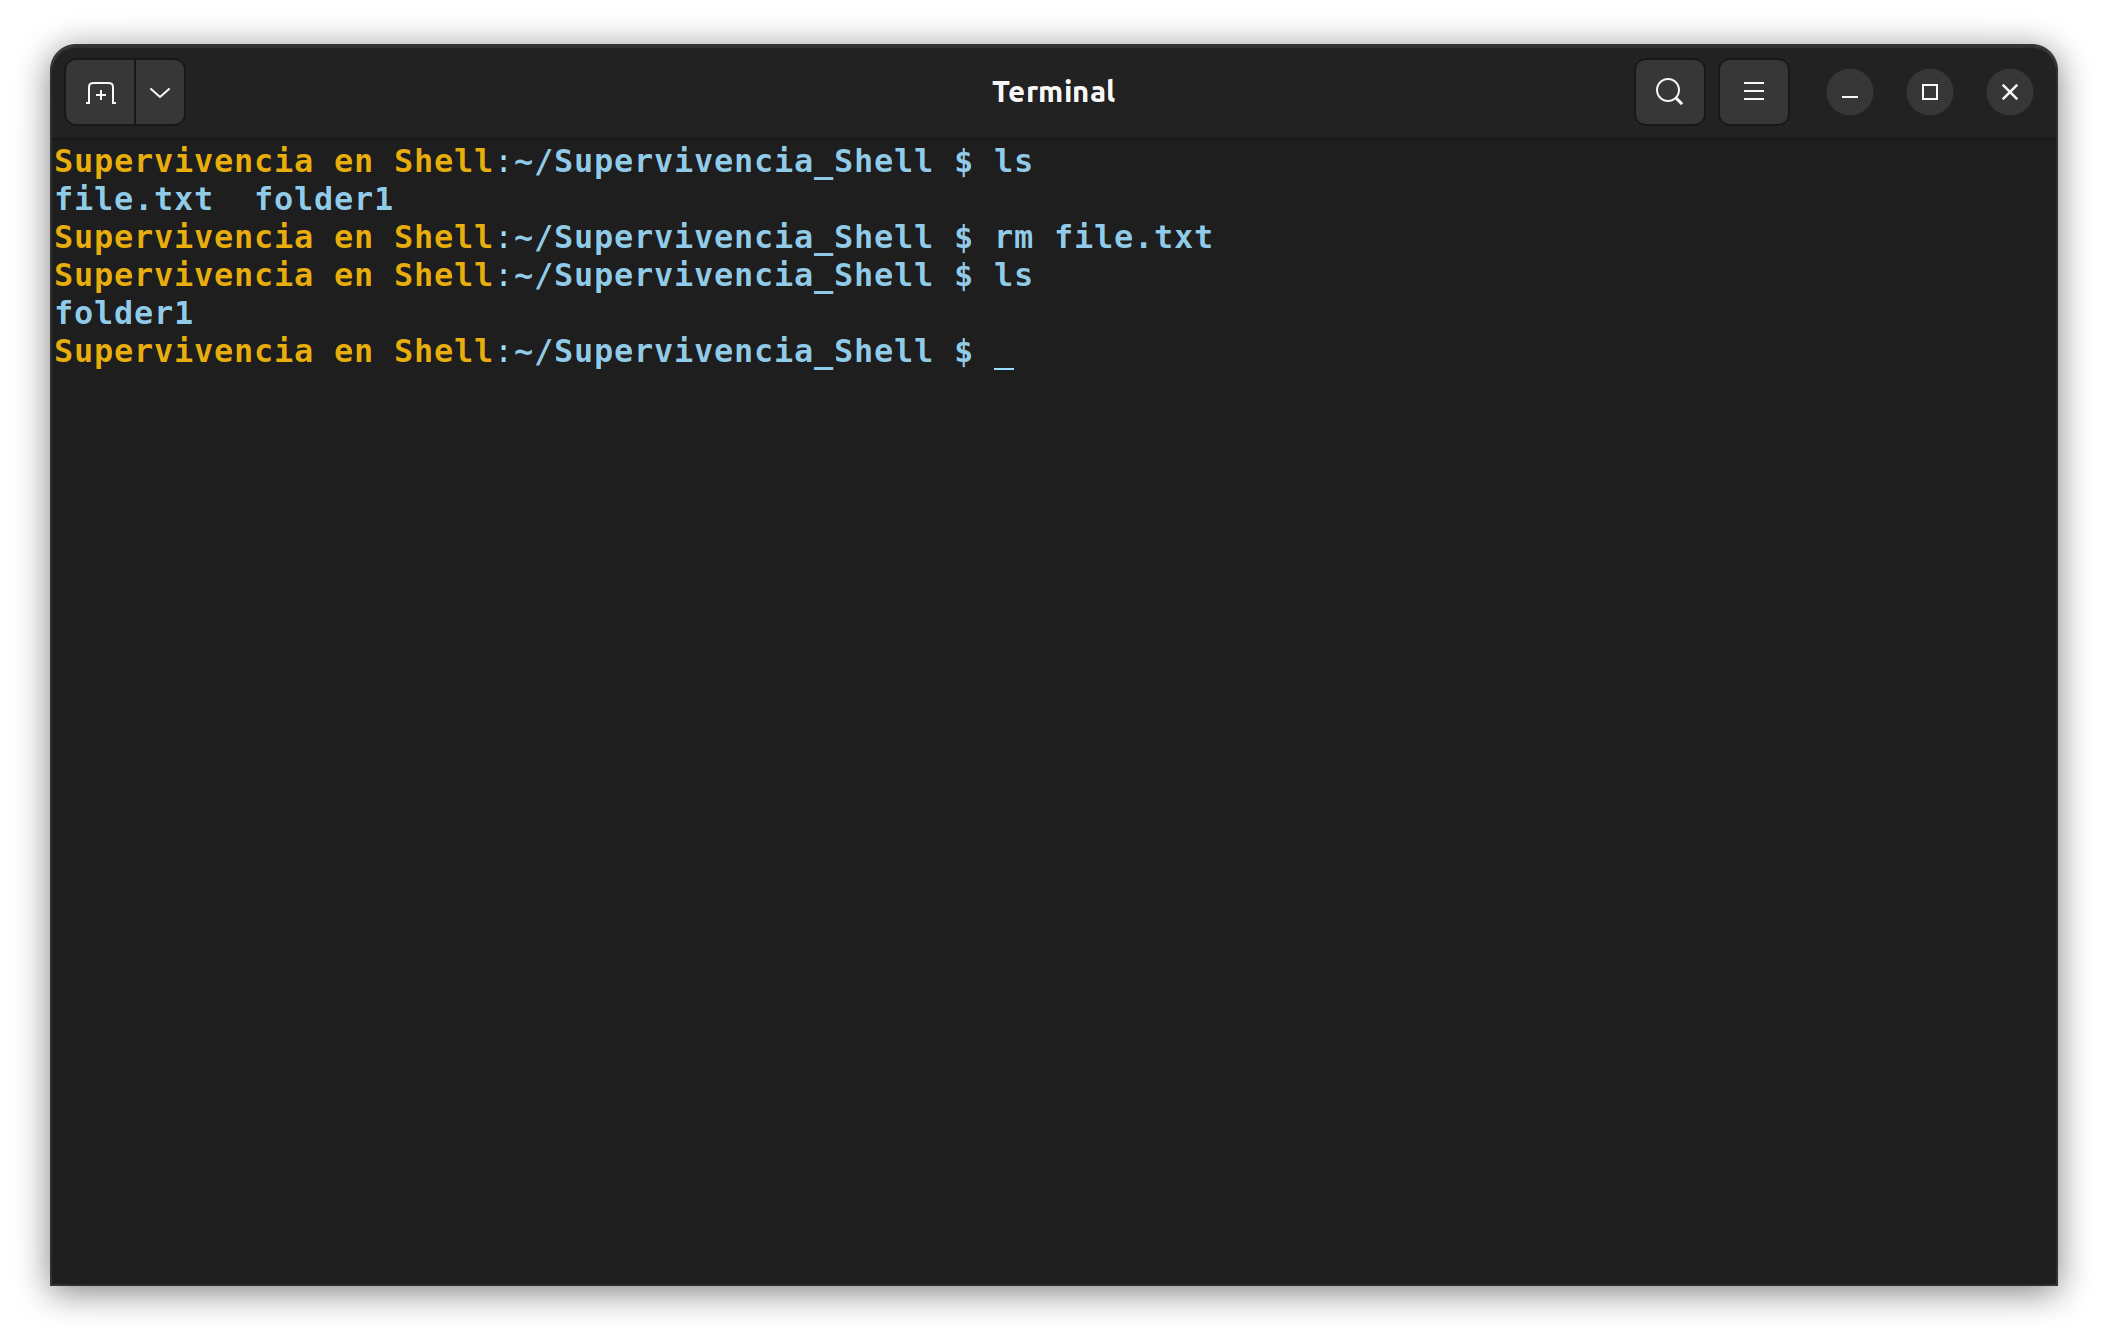
\includegraphics[width=0.55\textwidth]{rm}
		\end{center}
	\end{frame}	
		
	\begin{frame}
		\frametitle{Navegando por el terminal: mkdir}
		\begin{alertblock}{Crea directorios.}
			mkdir [OPTION]... DIRECTORY...
		\end{alertblock}
		\begin{center}
			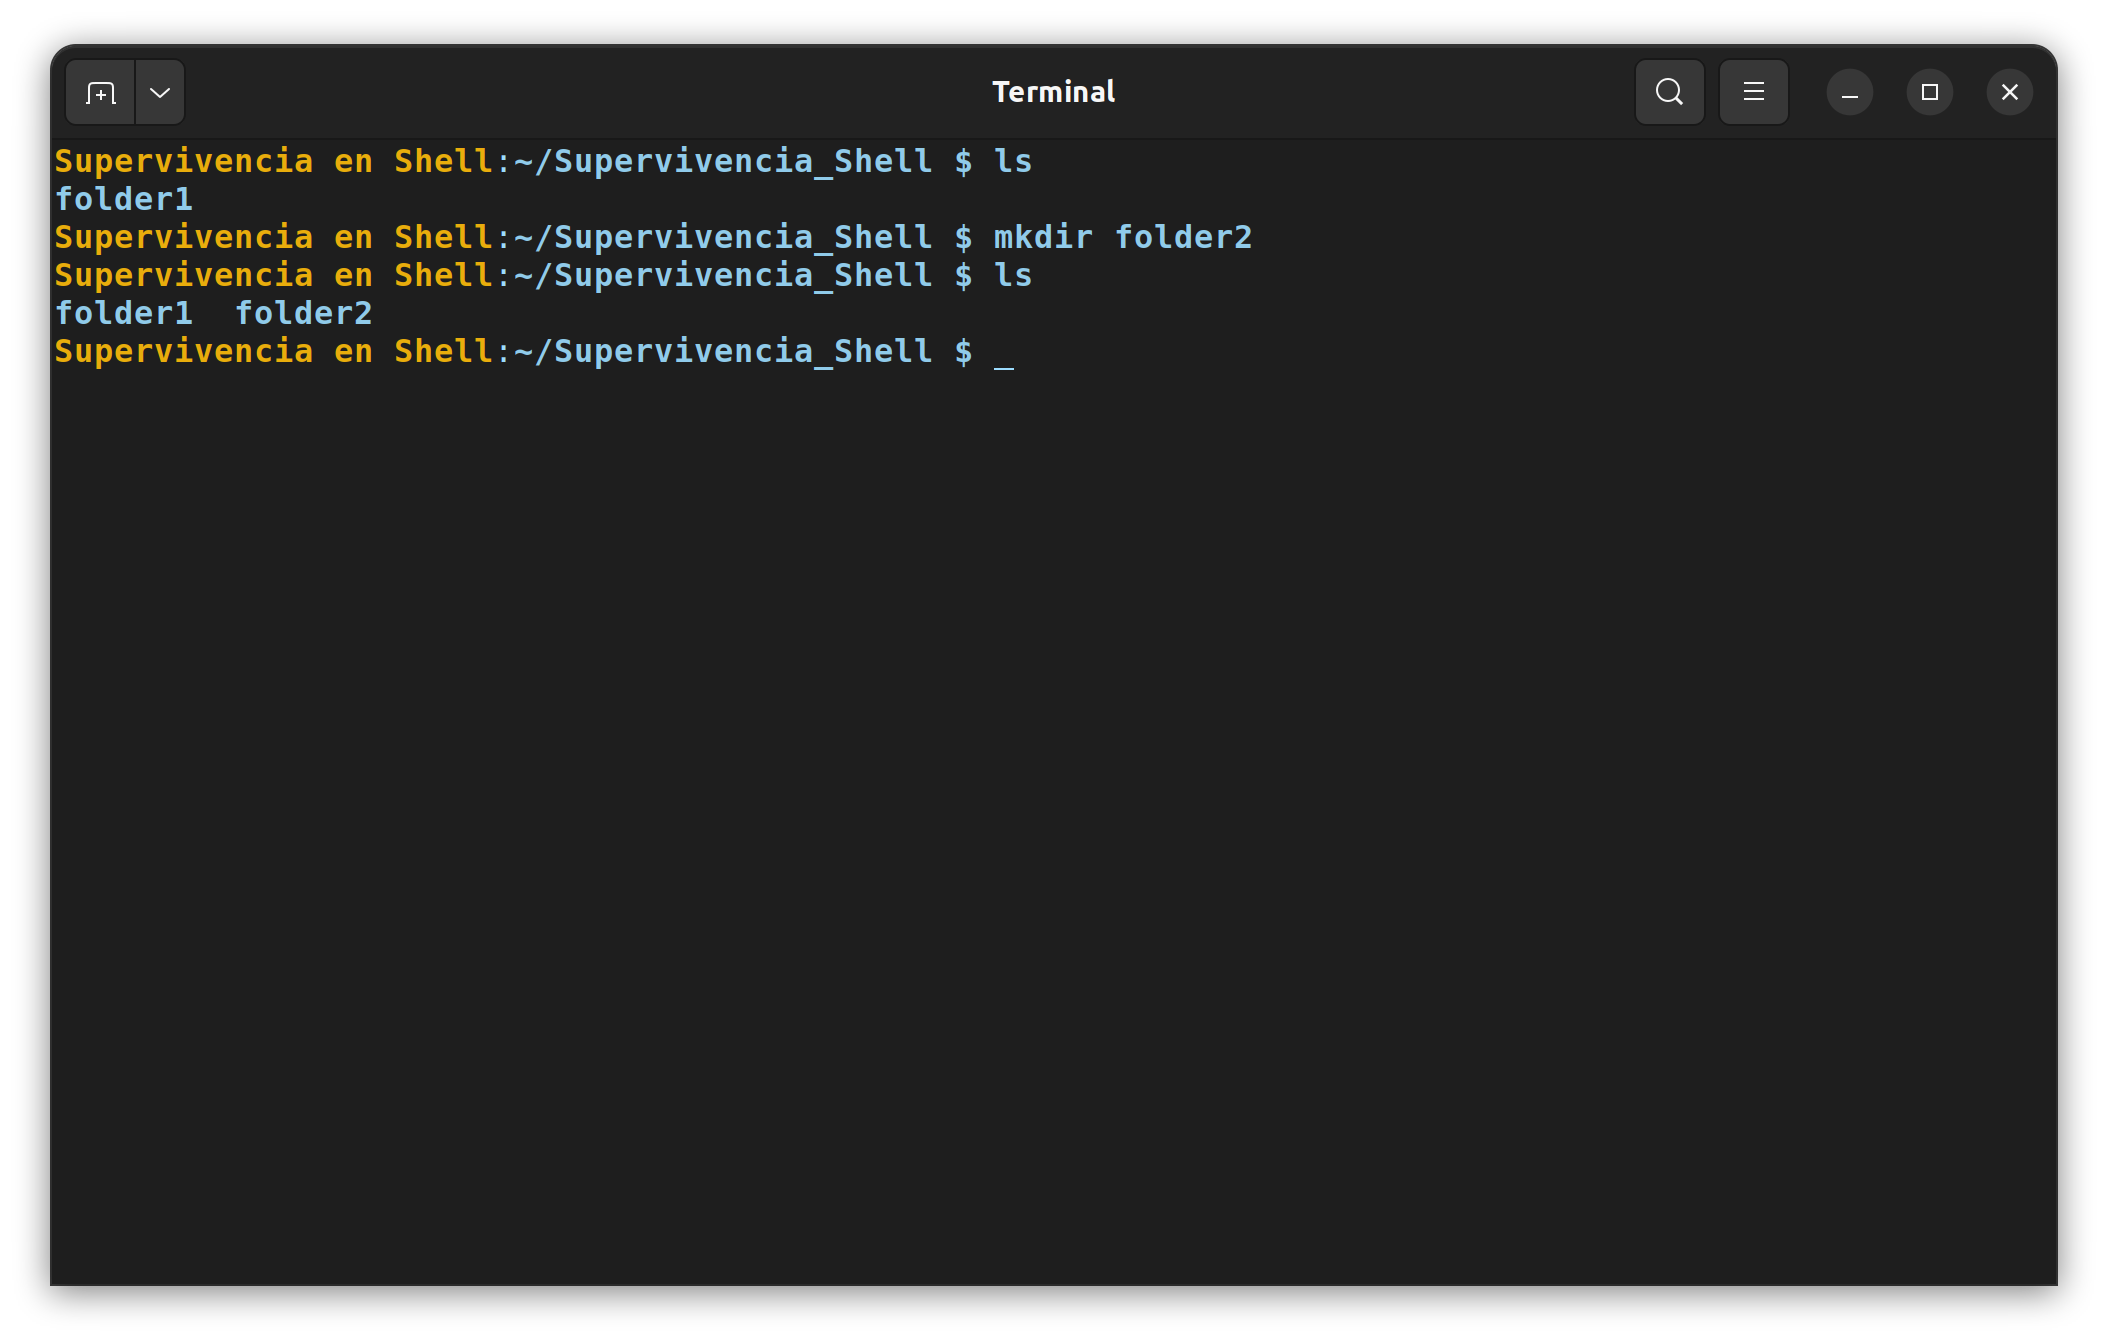
\includegraphics[width=0.55\textwidth]{mkdir}
		\end{center}
	\end{frame}	

	\begin{frame}
		\frametitle{Navegando por el terminal: rmdir}
		\begin{alertblock}{Borra directorios vacíos.}
			rmdir [OPTION]... DIRECTORY...
		\end{alertblock}
		\begin{center}
			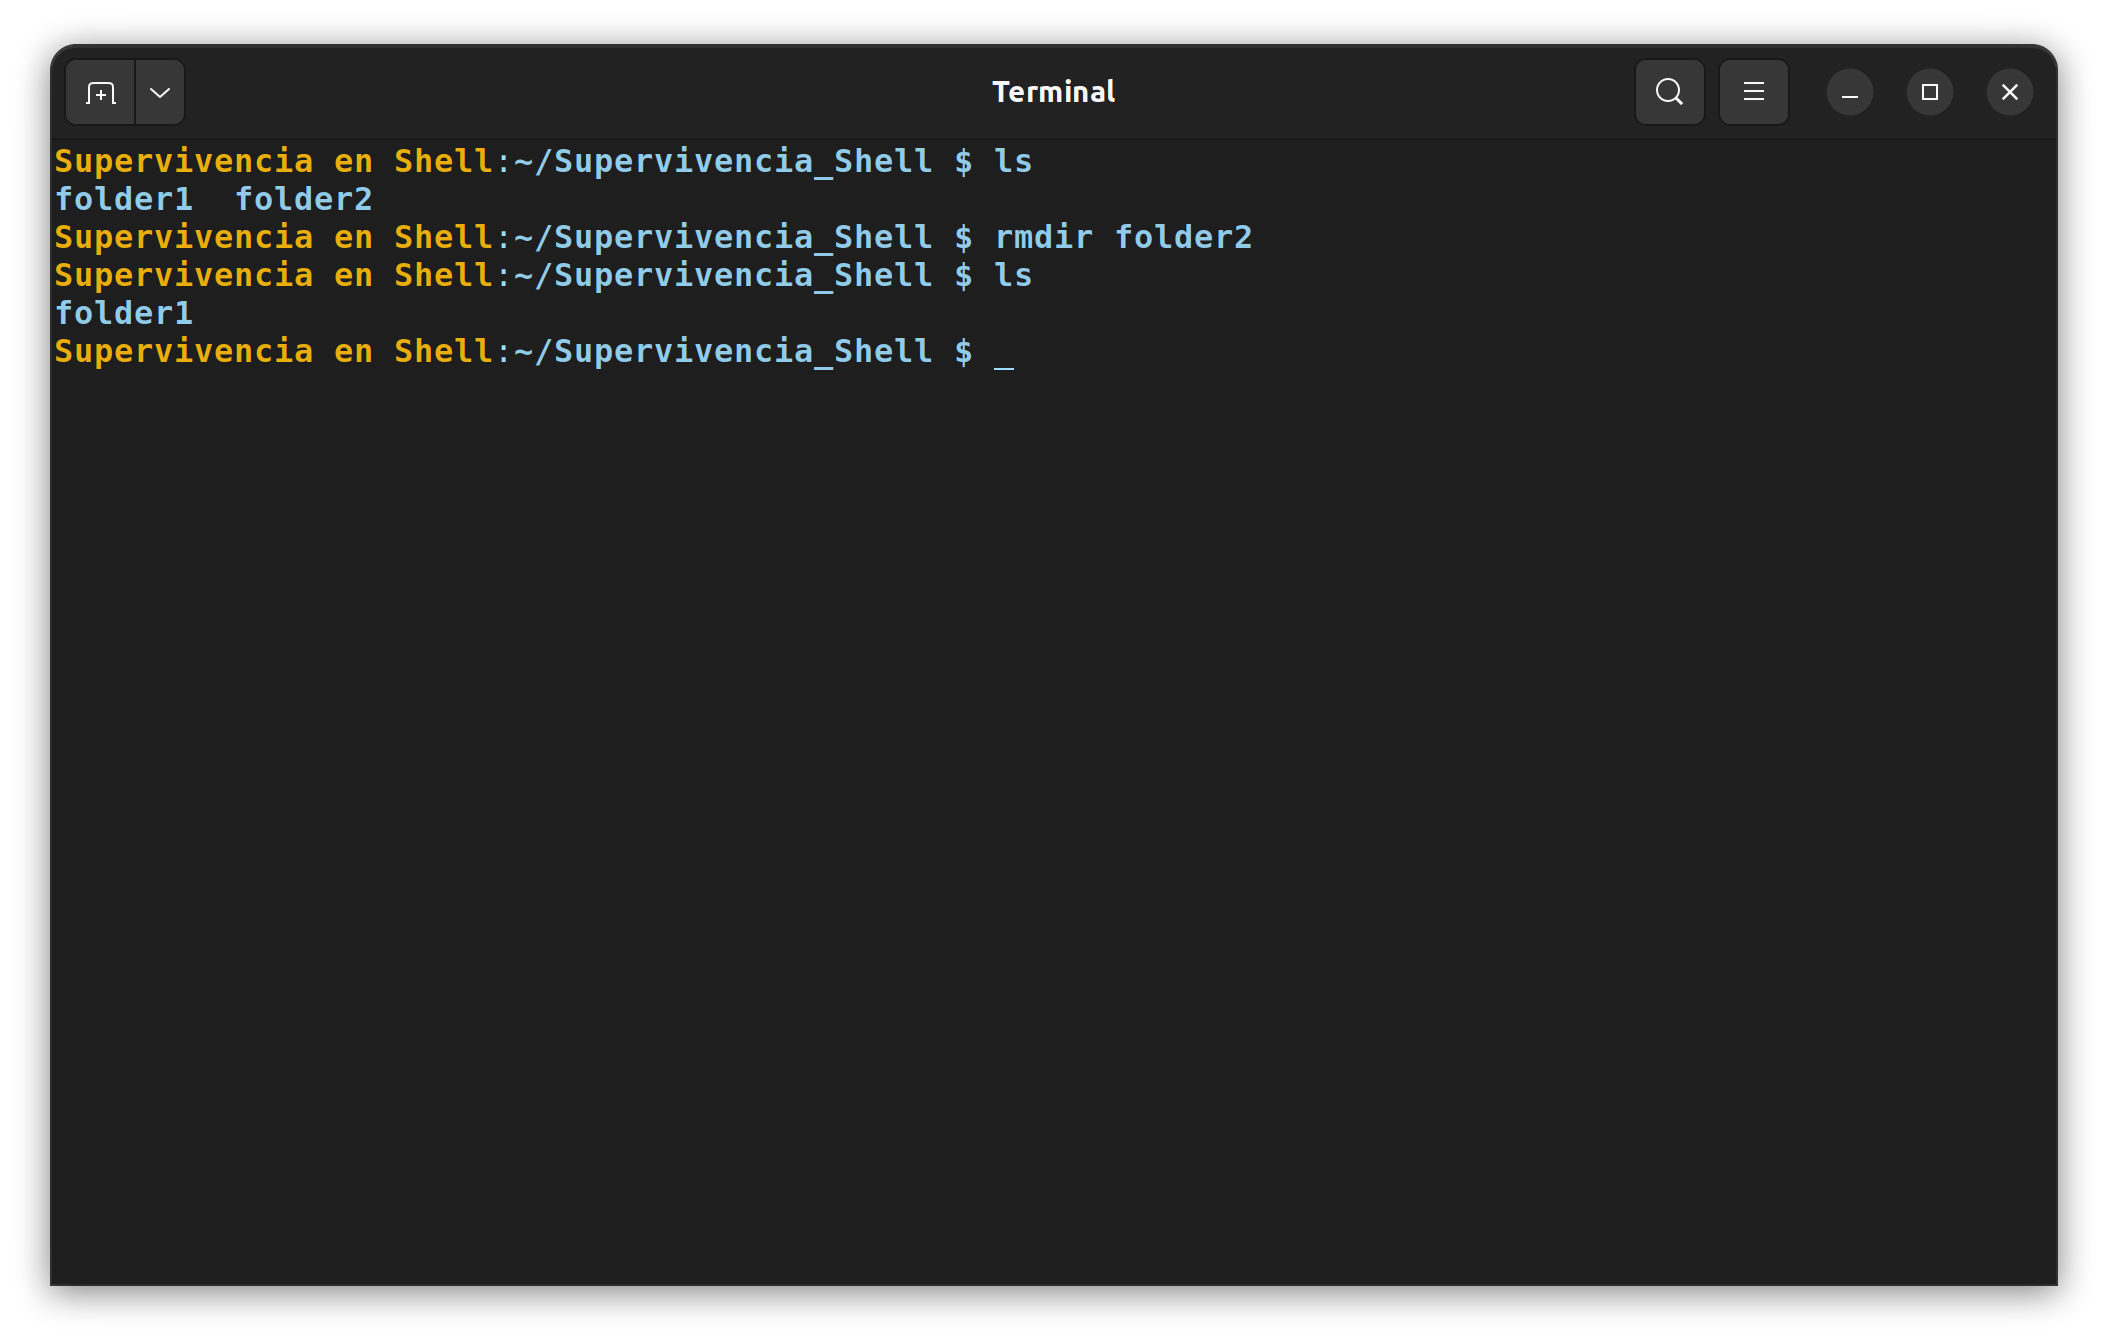
\includegraphics[width=0.55\textwidth]{rmdir}
		\end{center}
	\end{frame}
	
	\begin{frame}
		\frametitle{Visualizando ficheros: cat}
		\begin{alertblock}{Escribe en su salida el contenido de uno o varios ficheros.}
			cat [OPTION]... [FILE]...
		\end{alertblock}
		\begin{center}
			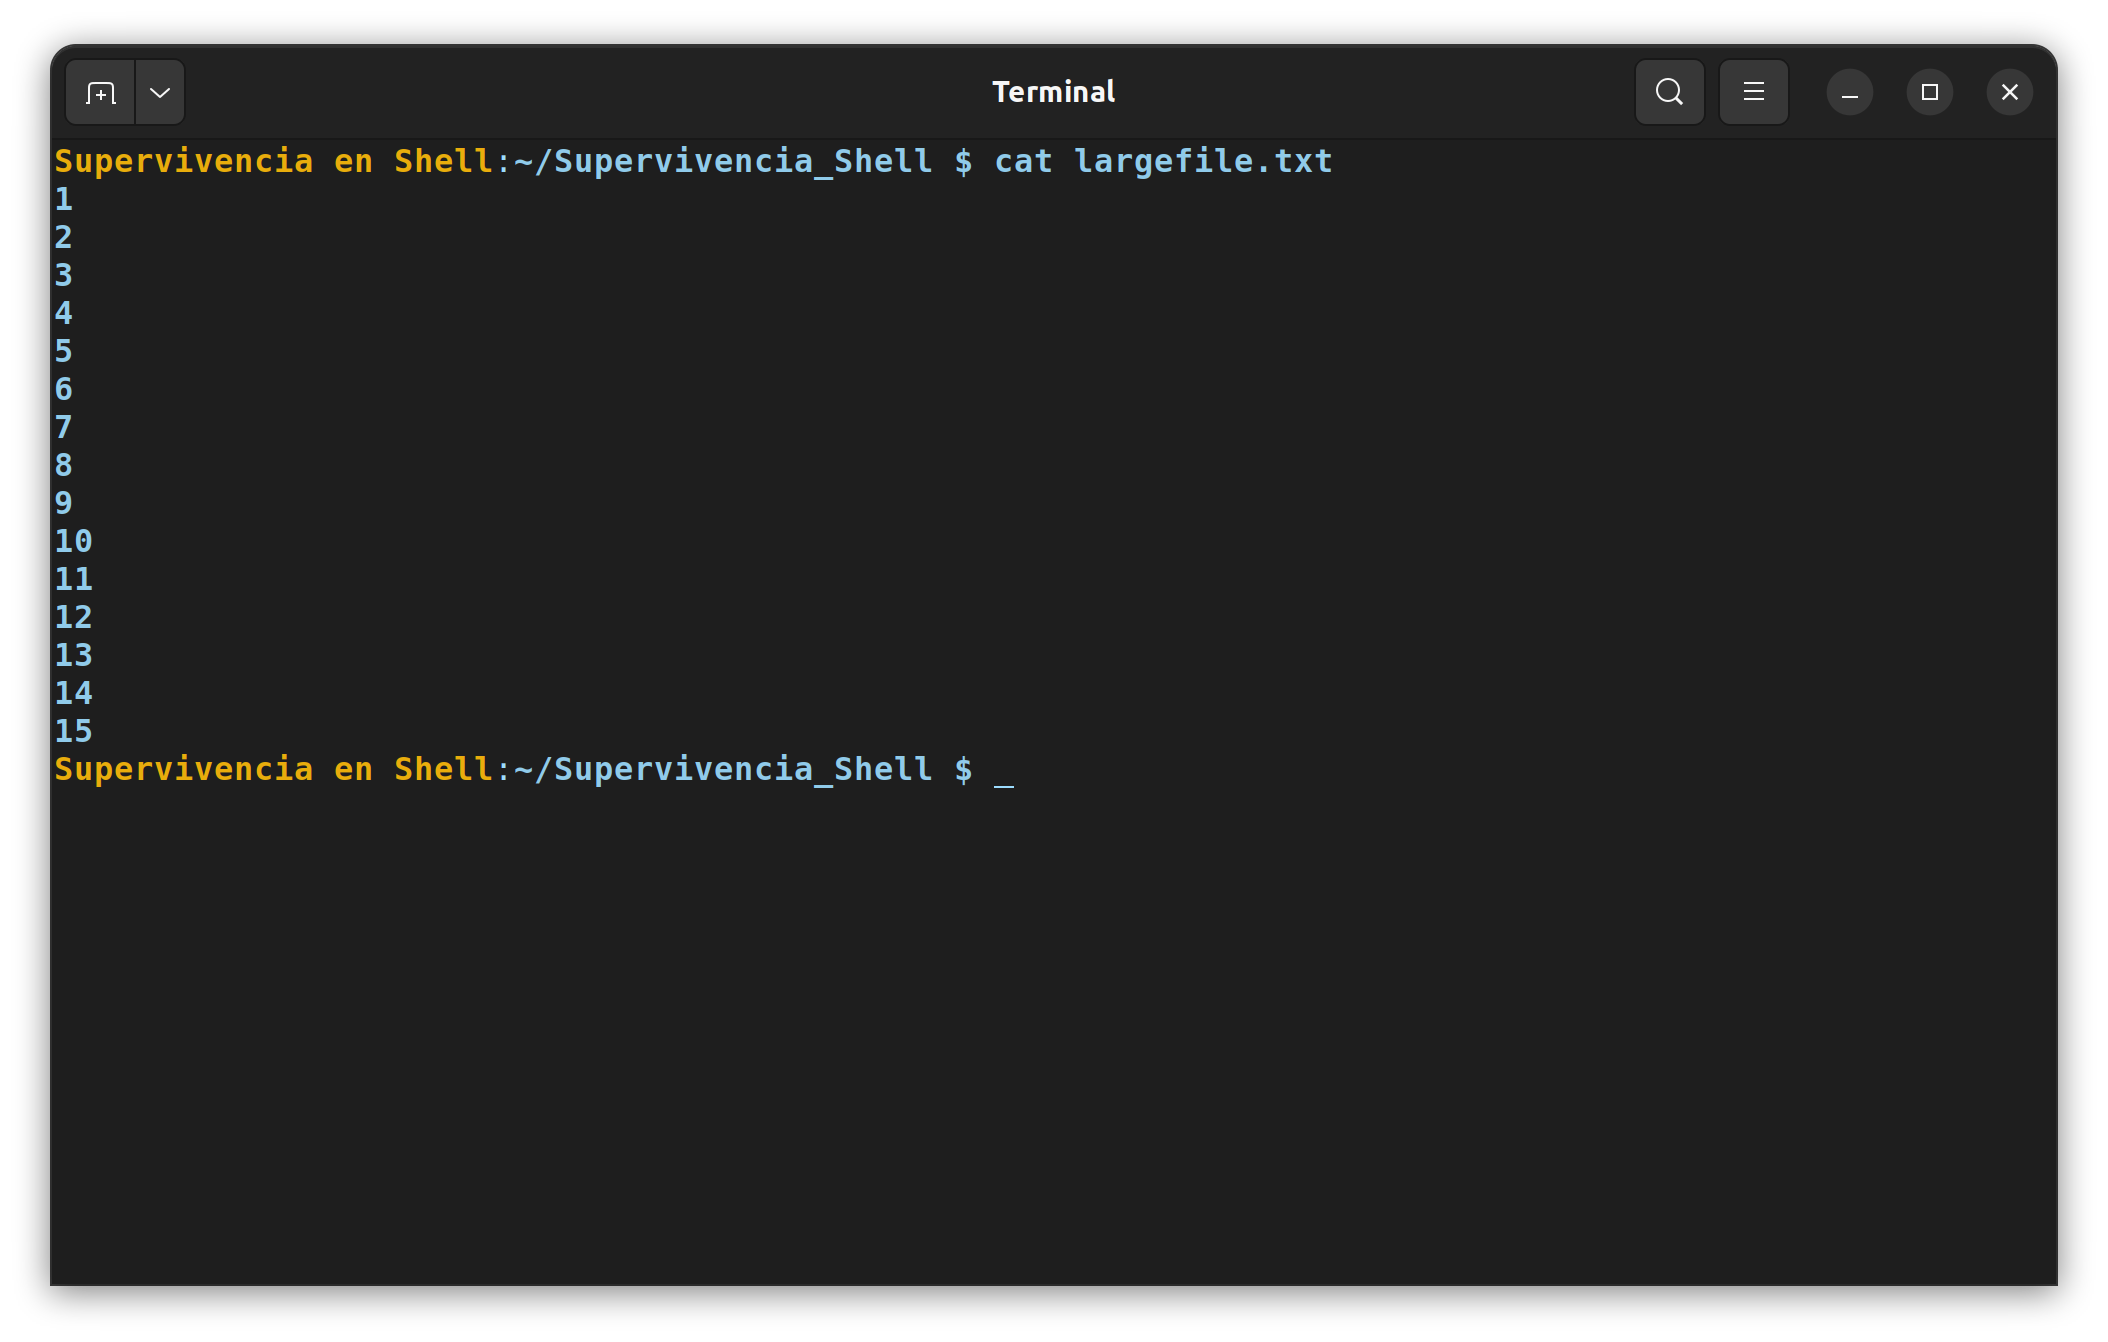
\includegraphics[width=0.55\textwidth]{cat}
		\end{center}
	\end{frame}	
	
	\begin{frame}
		\frametitle{Visualizando ficheros: less}
		\begin{alertblock}{Permite leer un fichero de texto en el terminal usando scroll.}
			less [FILE]
		\end{alertblock}
		\begin{center}
			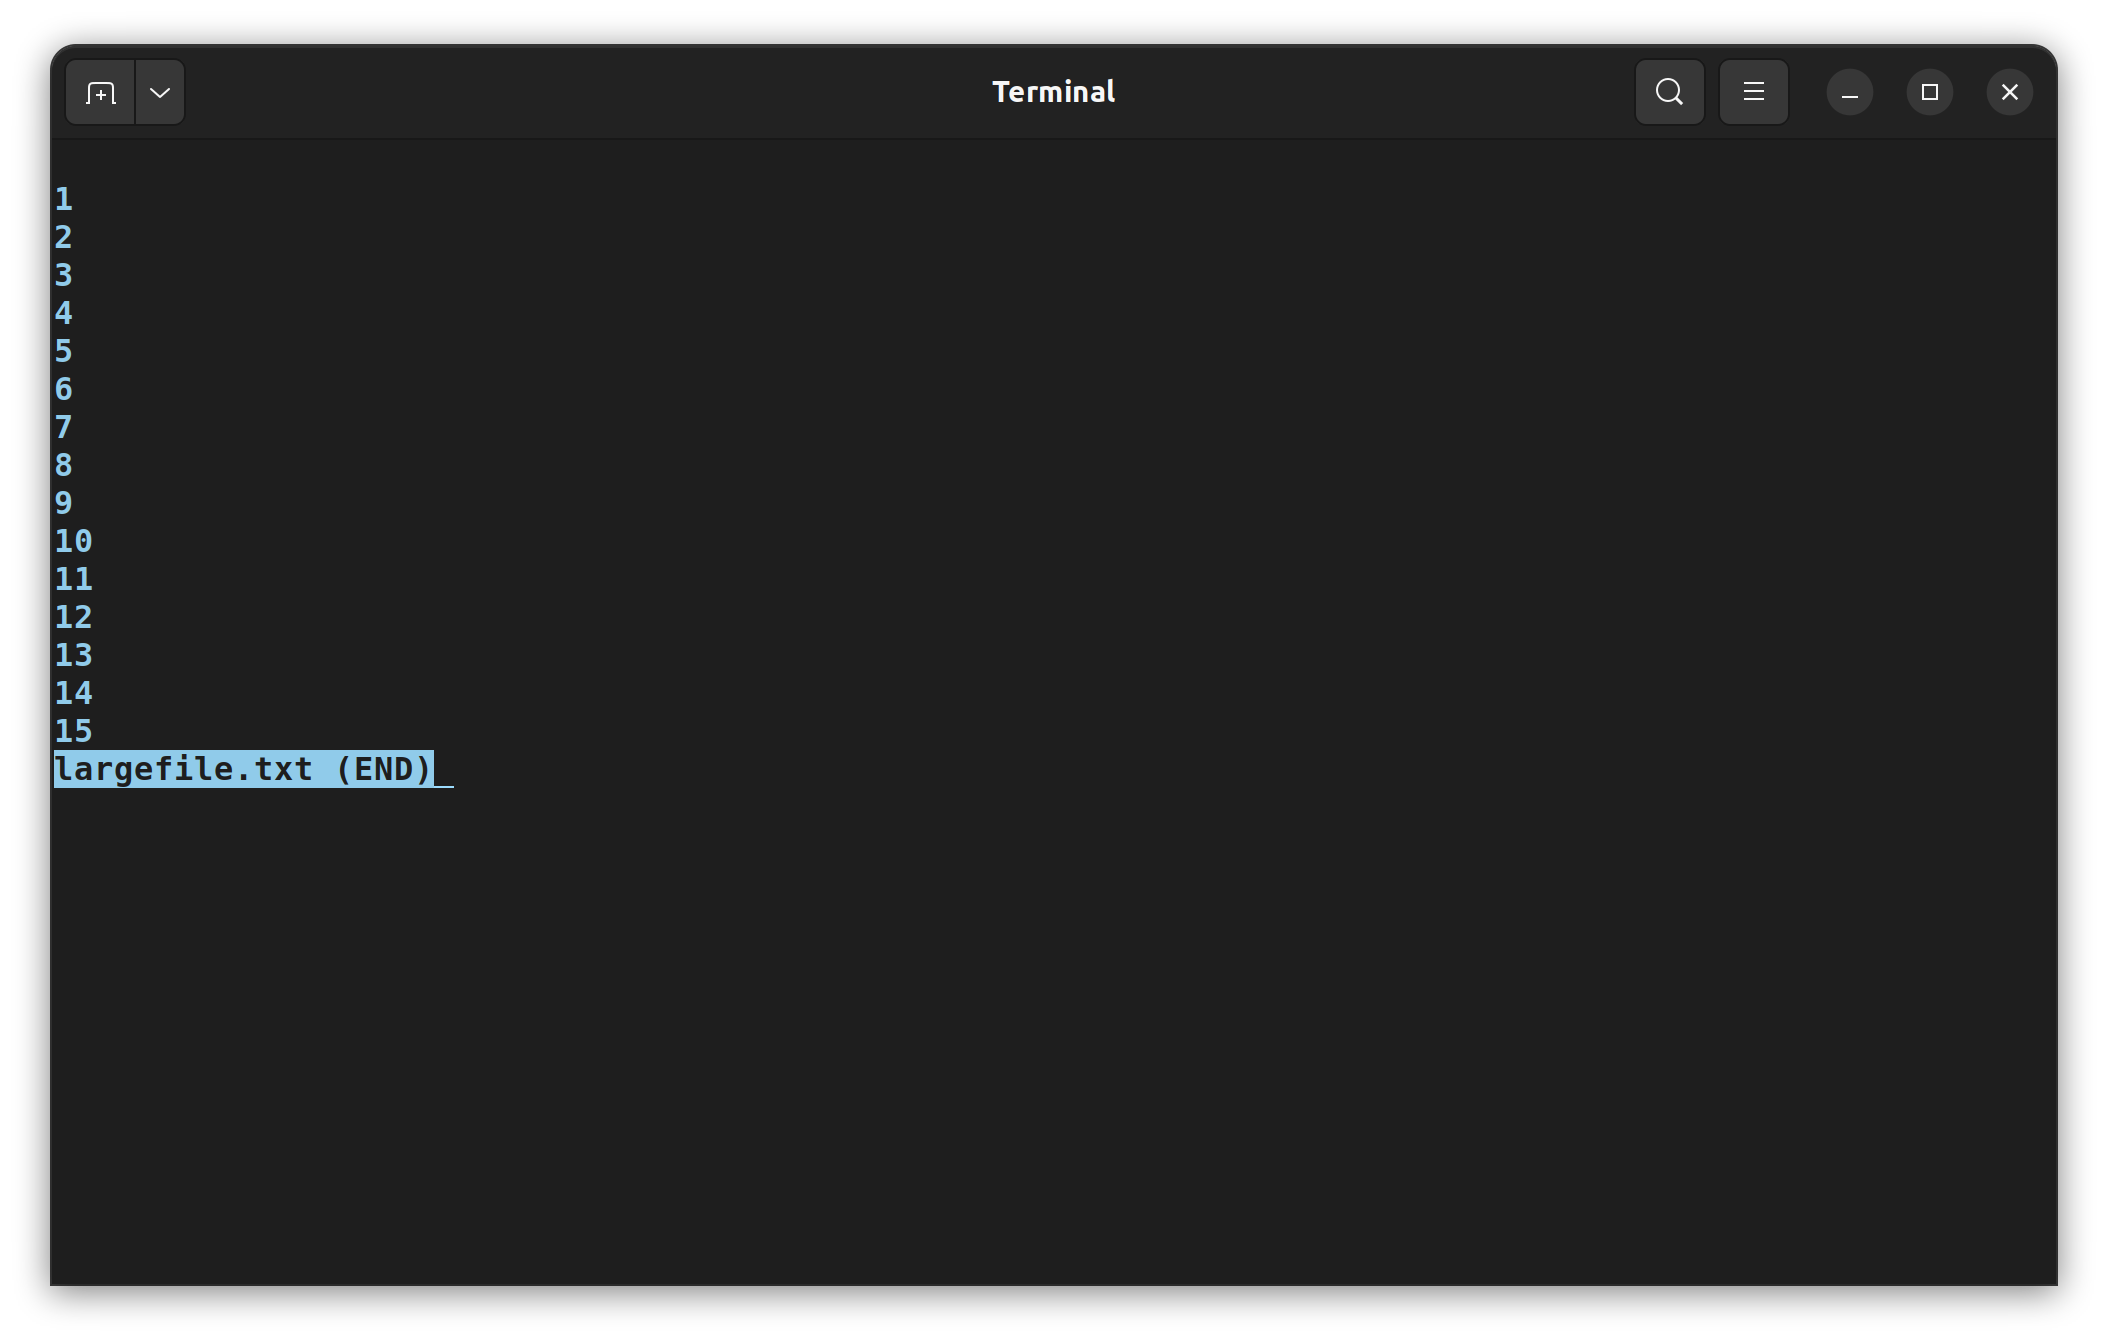
\includegraphics[width=0.55\textwidth]{less}
		\end{center}
	\end{frame}
		
	\begin{frame}
		\frametitle{Visualizando ficheros: head}
		\begin{alertblock}{Escribe las primeras líneas del fichero en su salida.}
			head [OPTION]... [FILE]...
		\end{alertblock}
		\begin{center}
			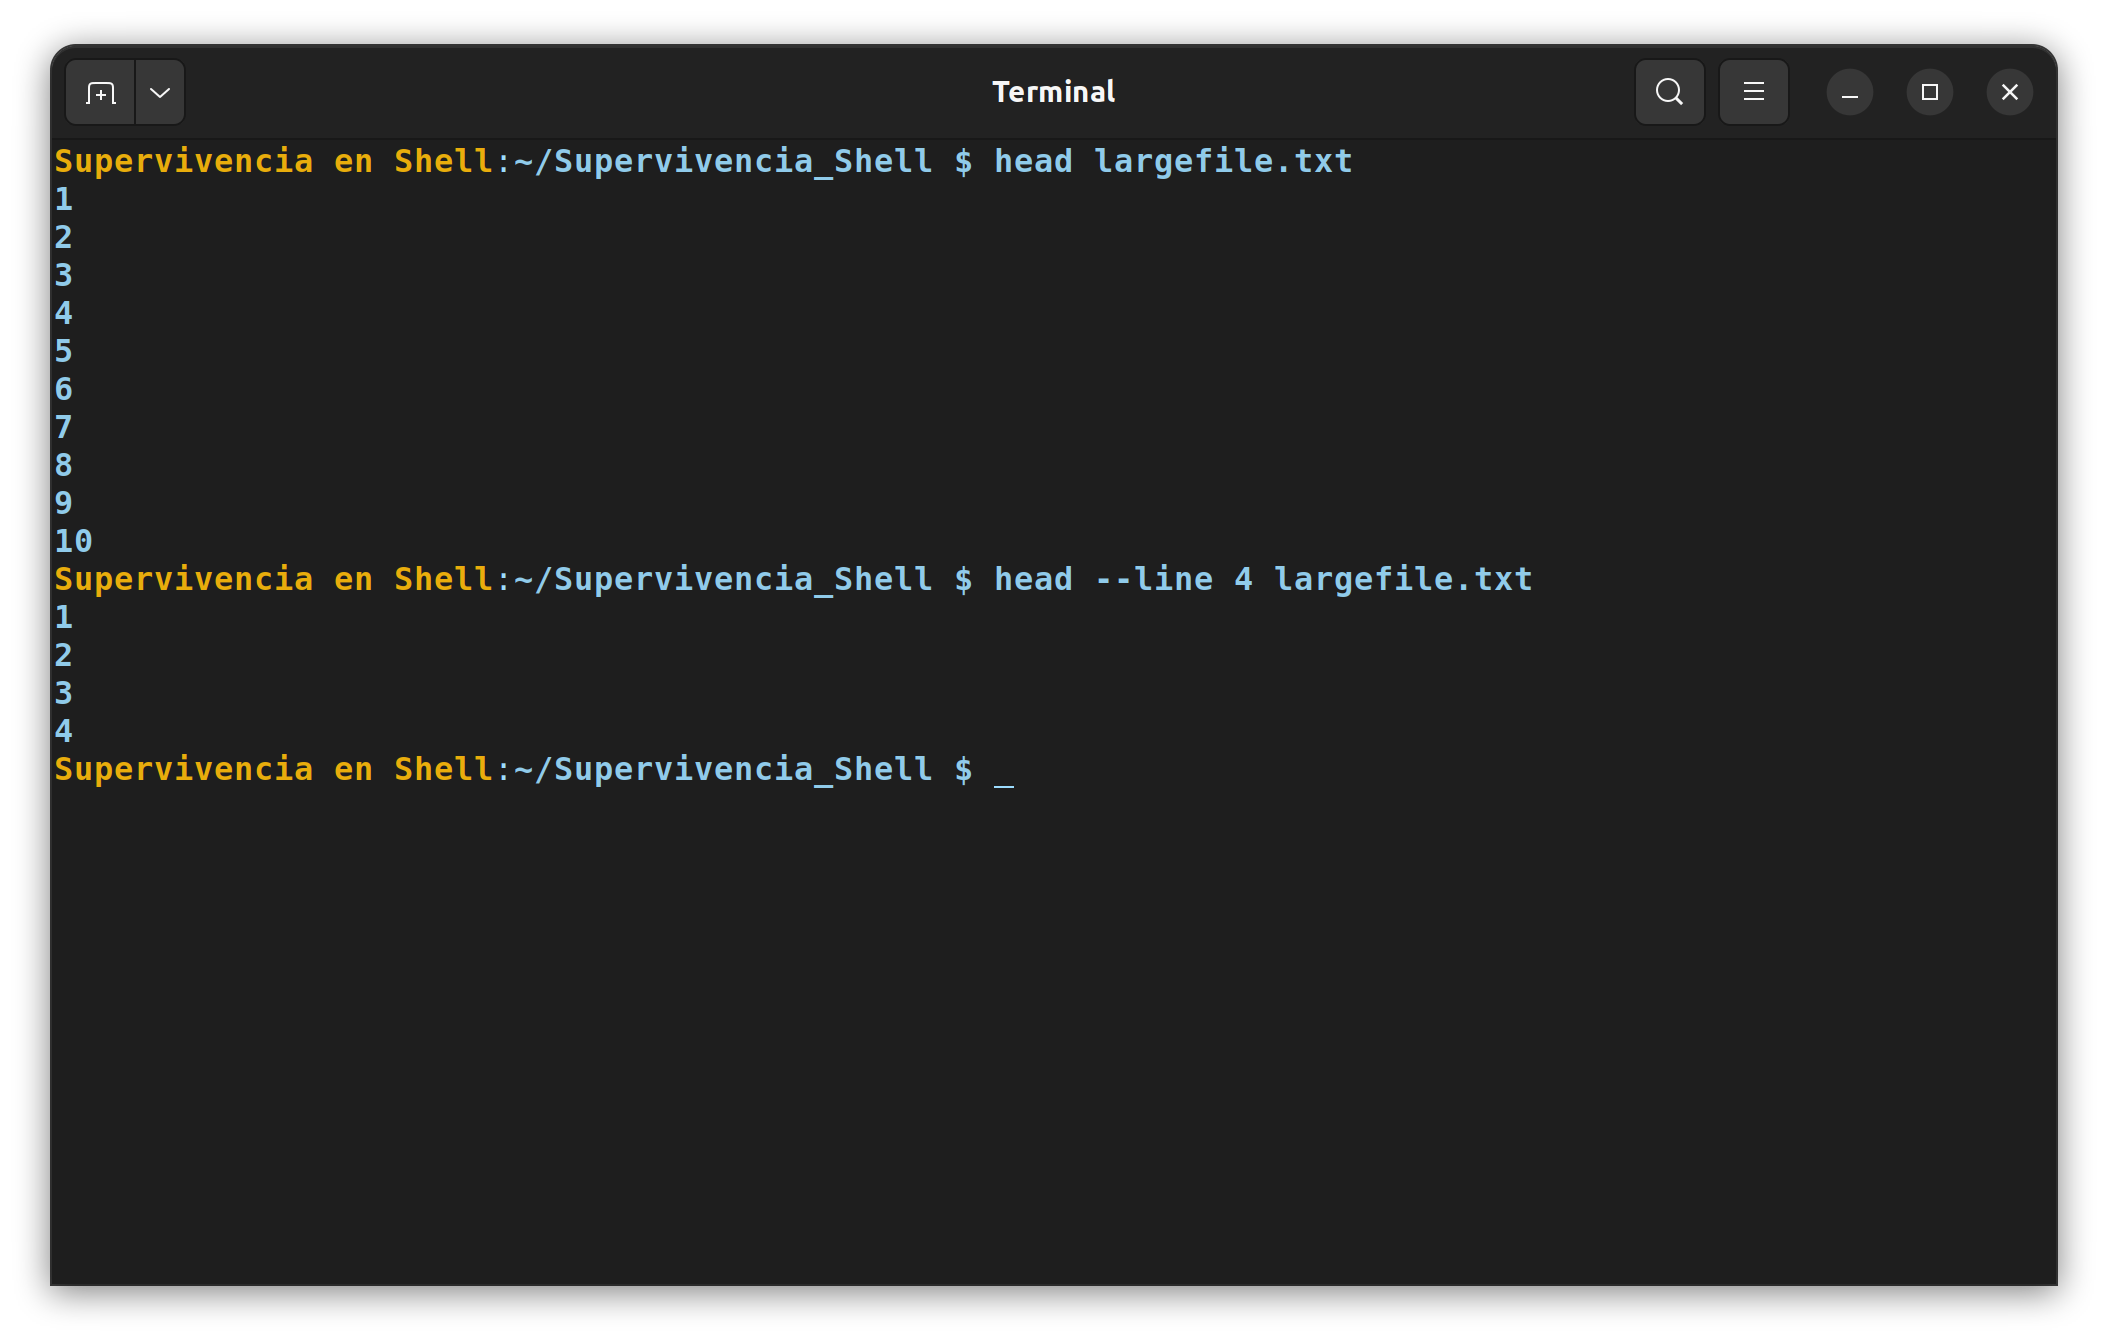
\includegraphics[width=0.55\textwidth]{head}
		\end{center}
	\end{frame}	
	
	\begin{frame}
		\frametitle{Visualizando ficheros: tail}
		\begin{alertblock}{Escribe las últimas líneas del fichero en su salida.}
			tail [OPTION]... [FILE]...
		\end{alertblock}
		\begin{center}
			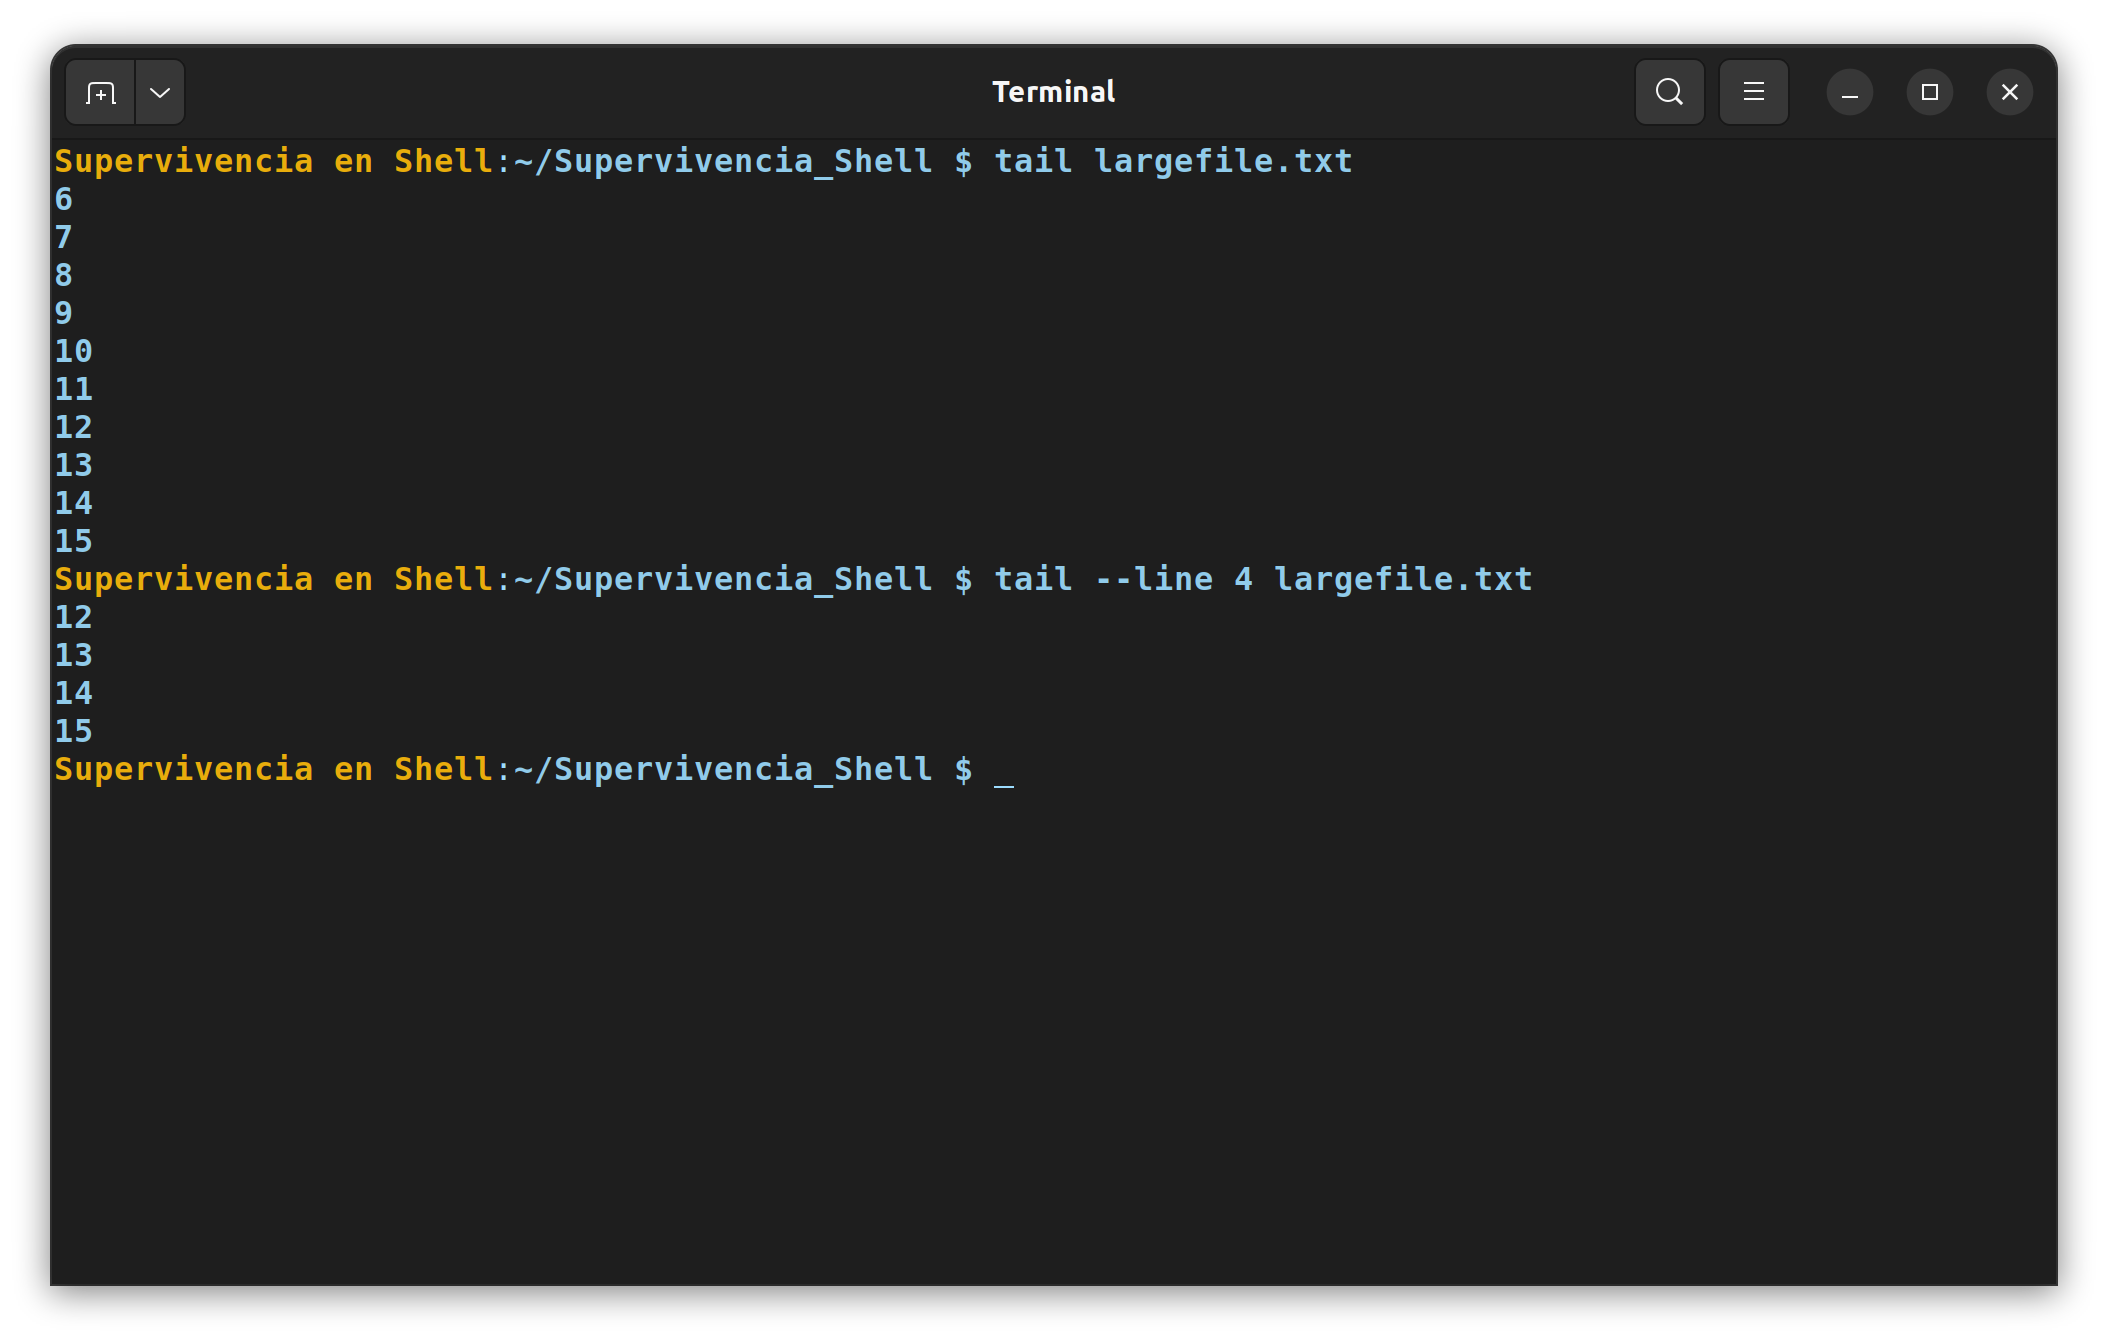
\includegraphics[width=0.55\textwidth]{tail}
		\end{center}
	\end{frame}
		
	\begin{frame}
		\frametitle{Visualizando ficheros: file}
		\begin{alertblock}{Da pistas sobre el contenido de un fichero.}
			file FILE
		\end{alertblock}
		\begin{center}
			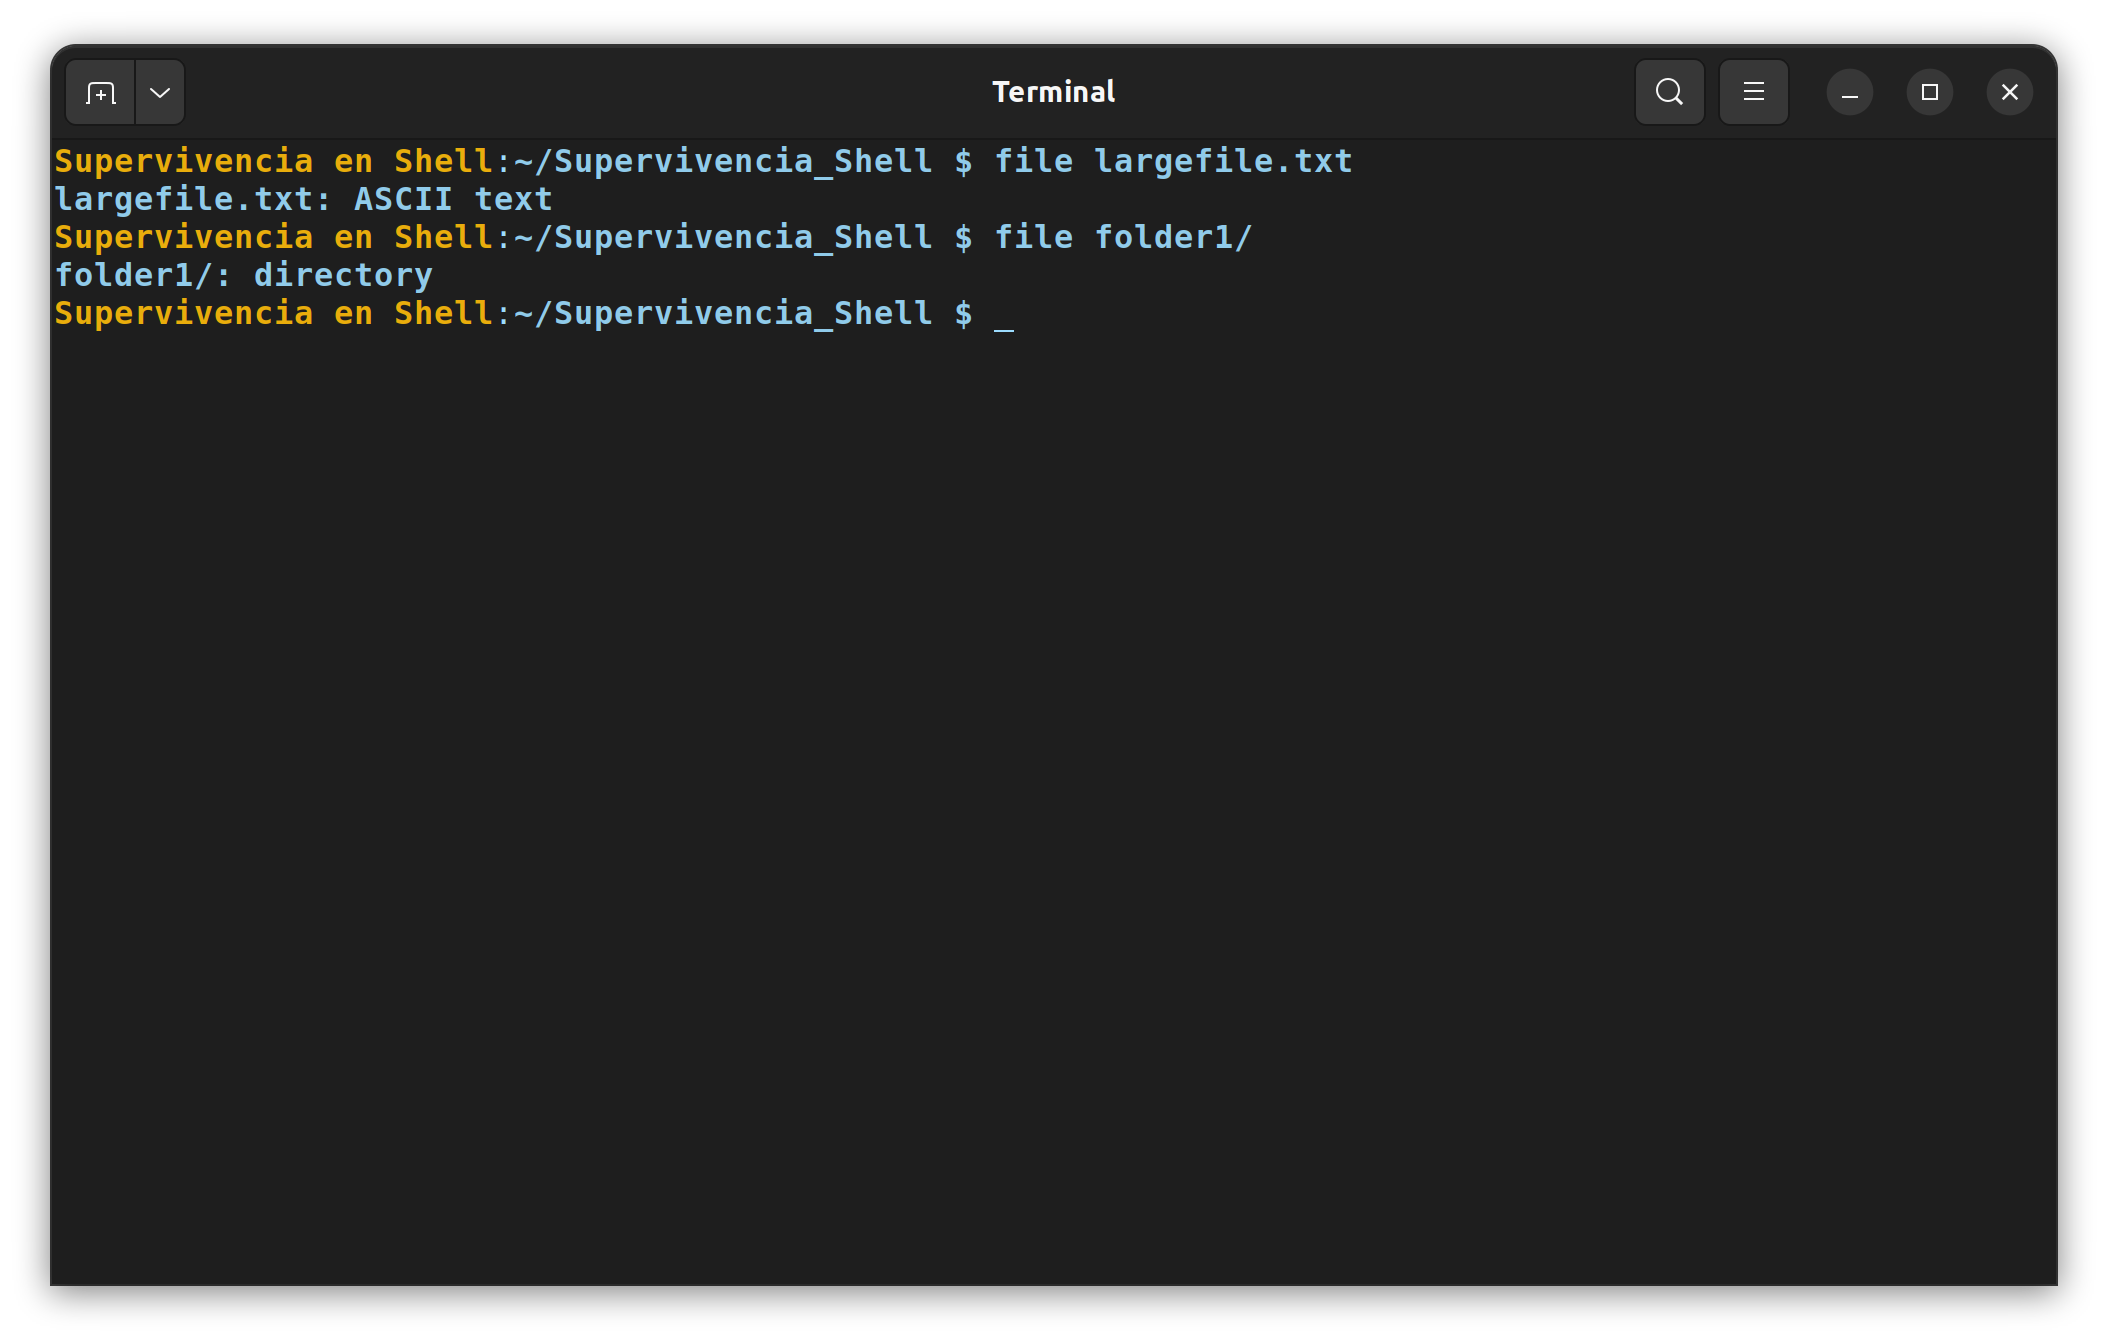
\includegraphics[width=0.55\textwidth]{file}
		\end{center}
	\end{frame}
		
	\begin{frame}
		\frametitle{Buscando en ficheros: grep/fgrep}
		\begin{alertblock}{Buscan cadenas dentro de ficheros.}
			grep [OPTION...] PATTERNS [FILE...]
		\end{alertblock}
		\begin{center}
			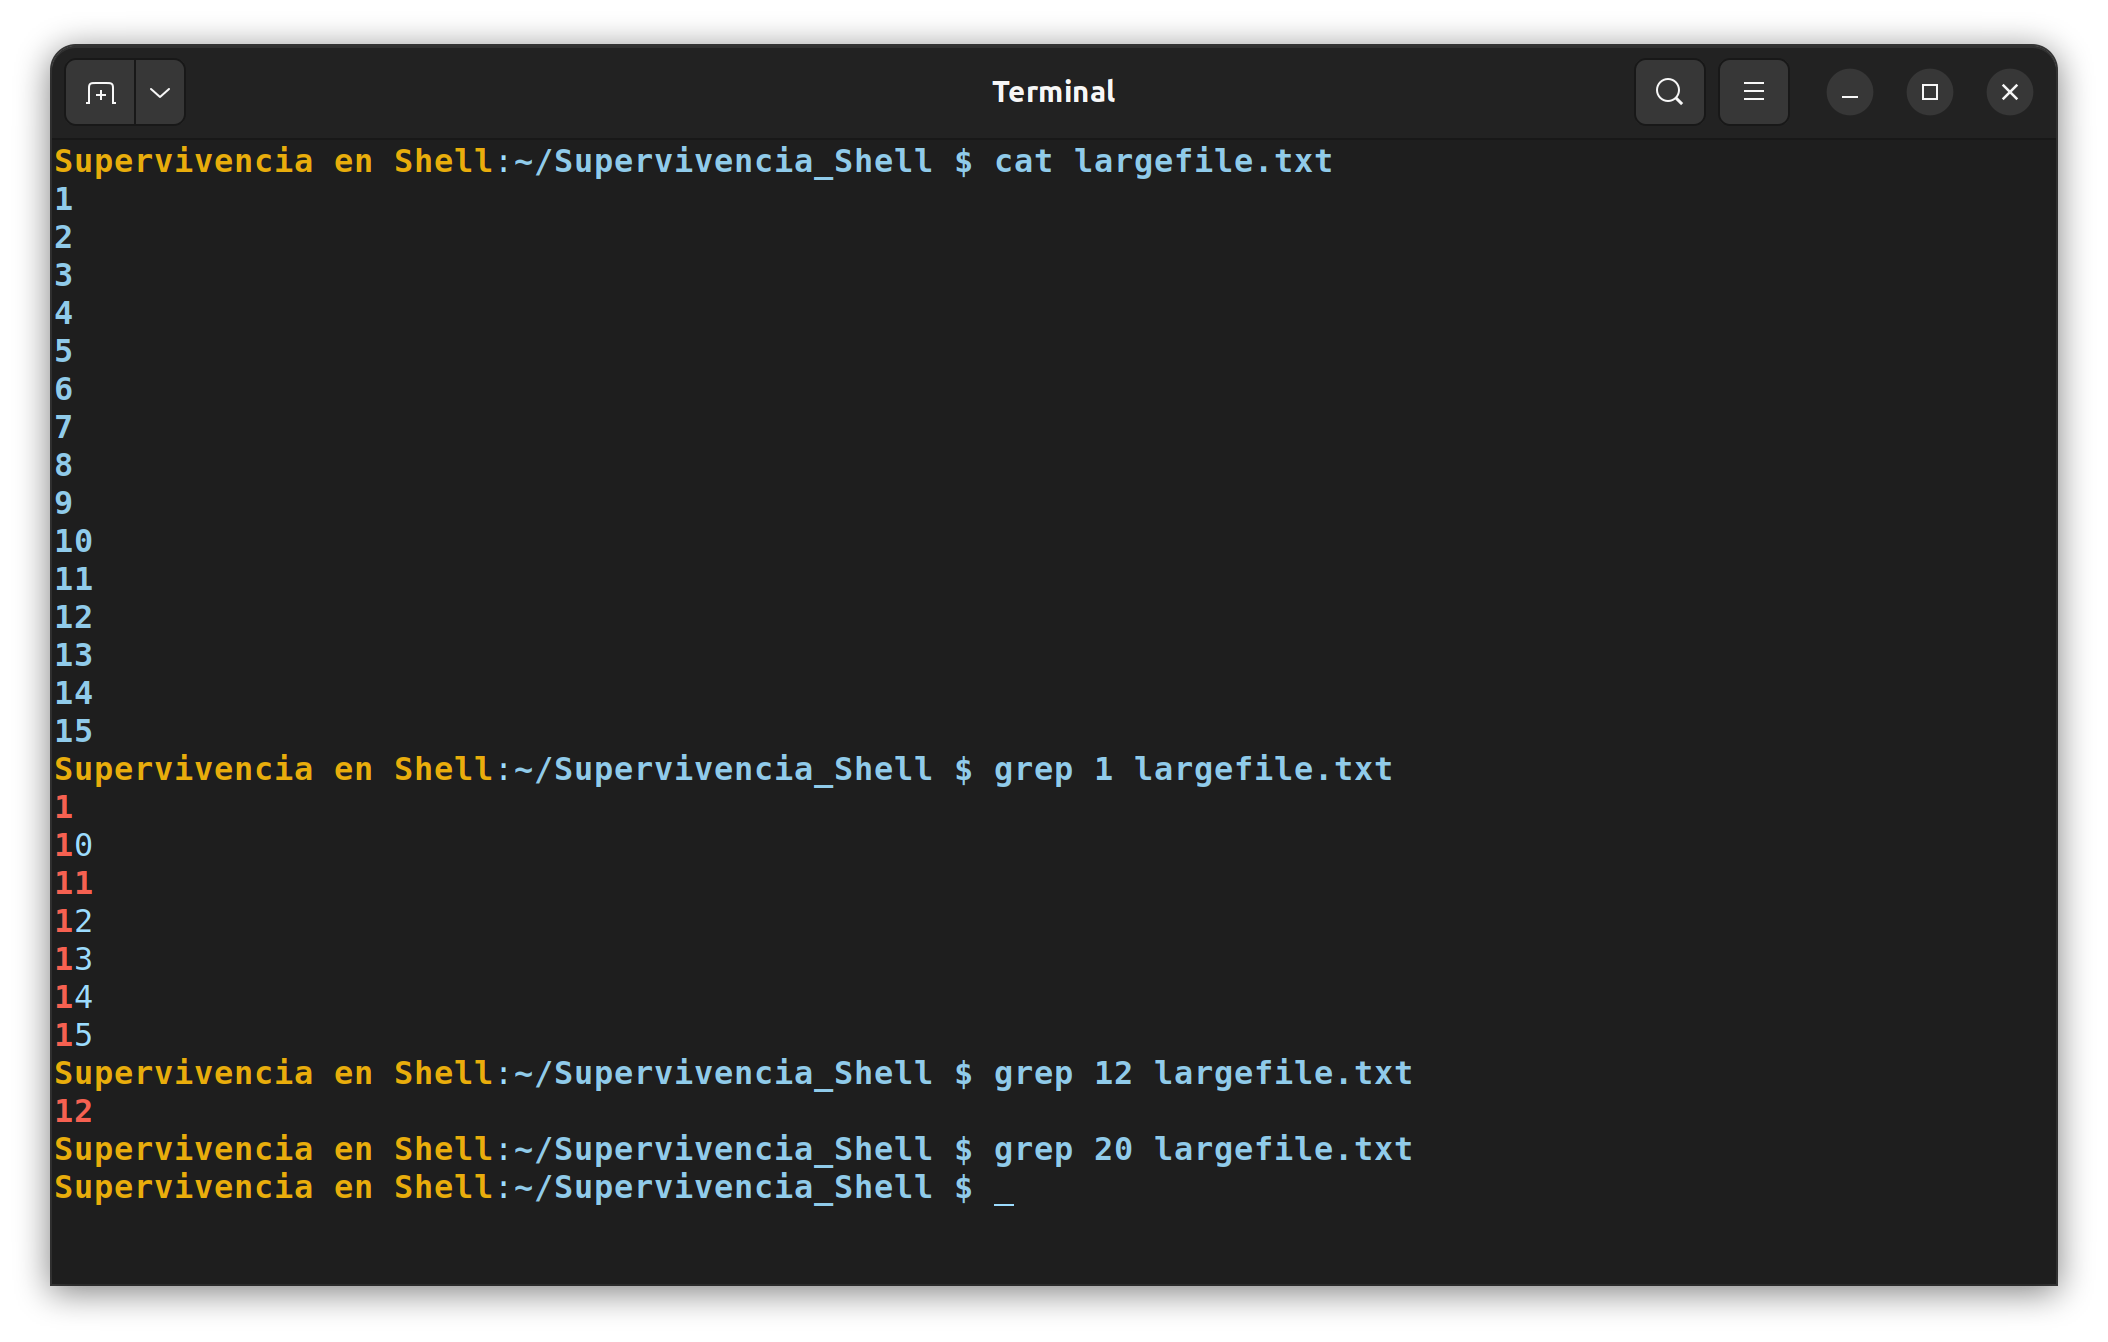
\includegraphics[width=0.55\textwidth]{grep}
		\end{center}
	\end{frame}
	
	\begin{frame}
		\frametitle{Ordenando ficheros: sort}
		\begin{alertblock}{Ordena las líneas de un fichero.}
			sort [OPTION]... [FILE]...
		\end{alertblock}
		\begin{center}
			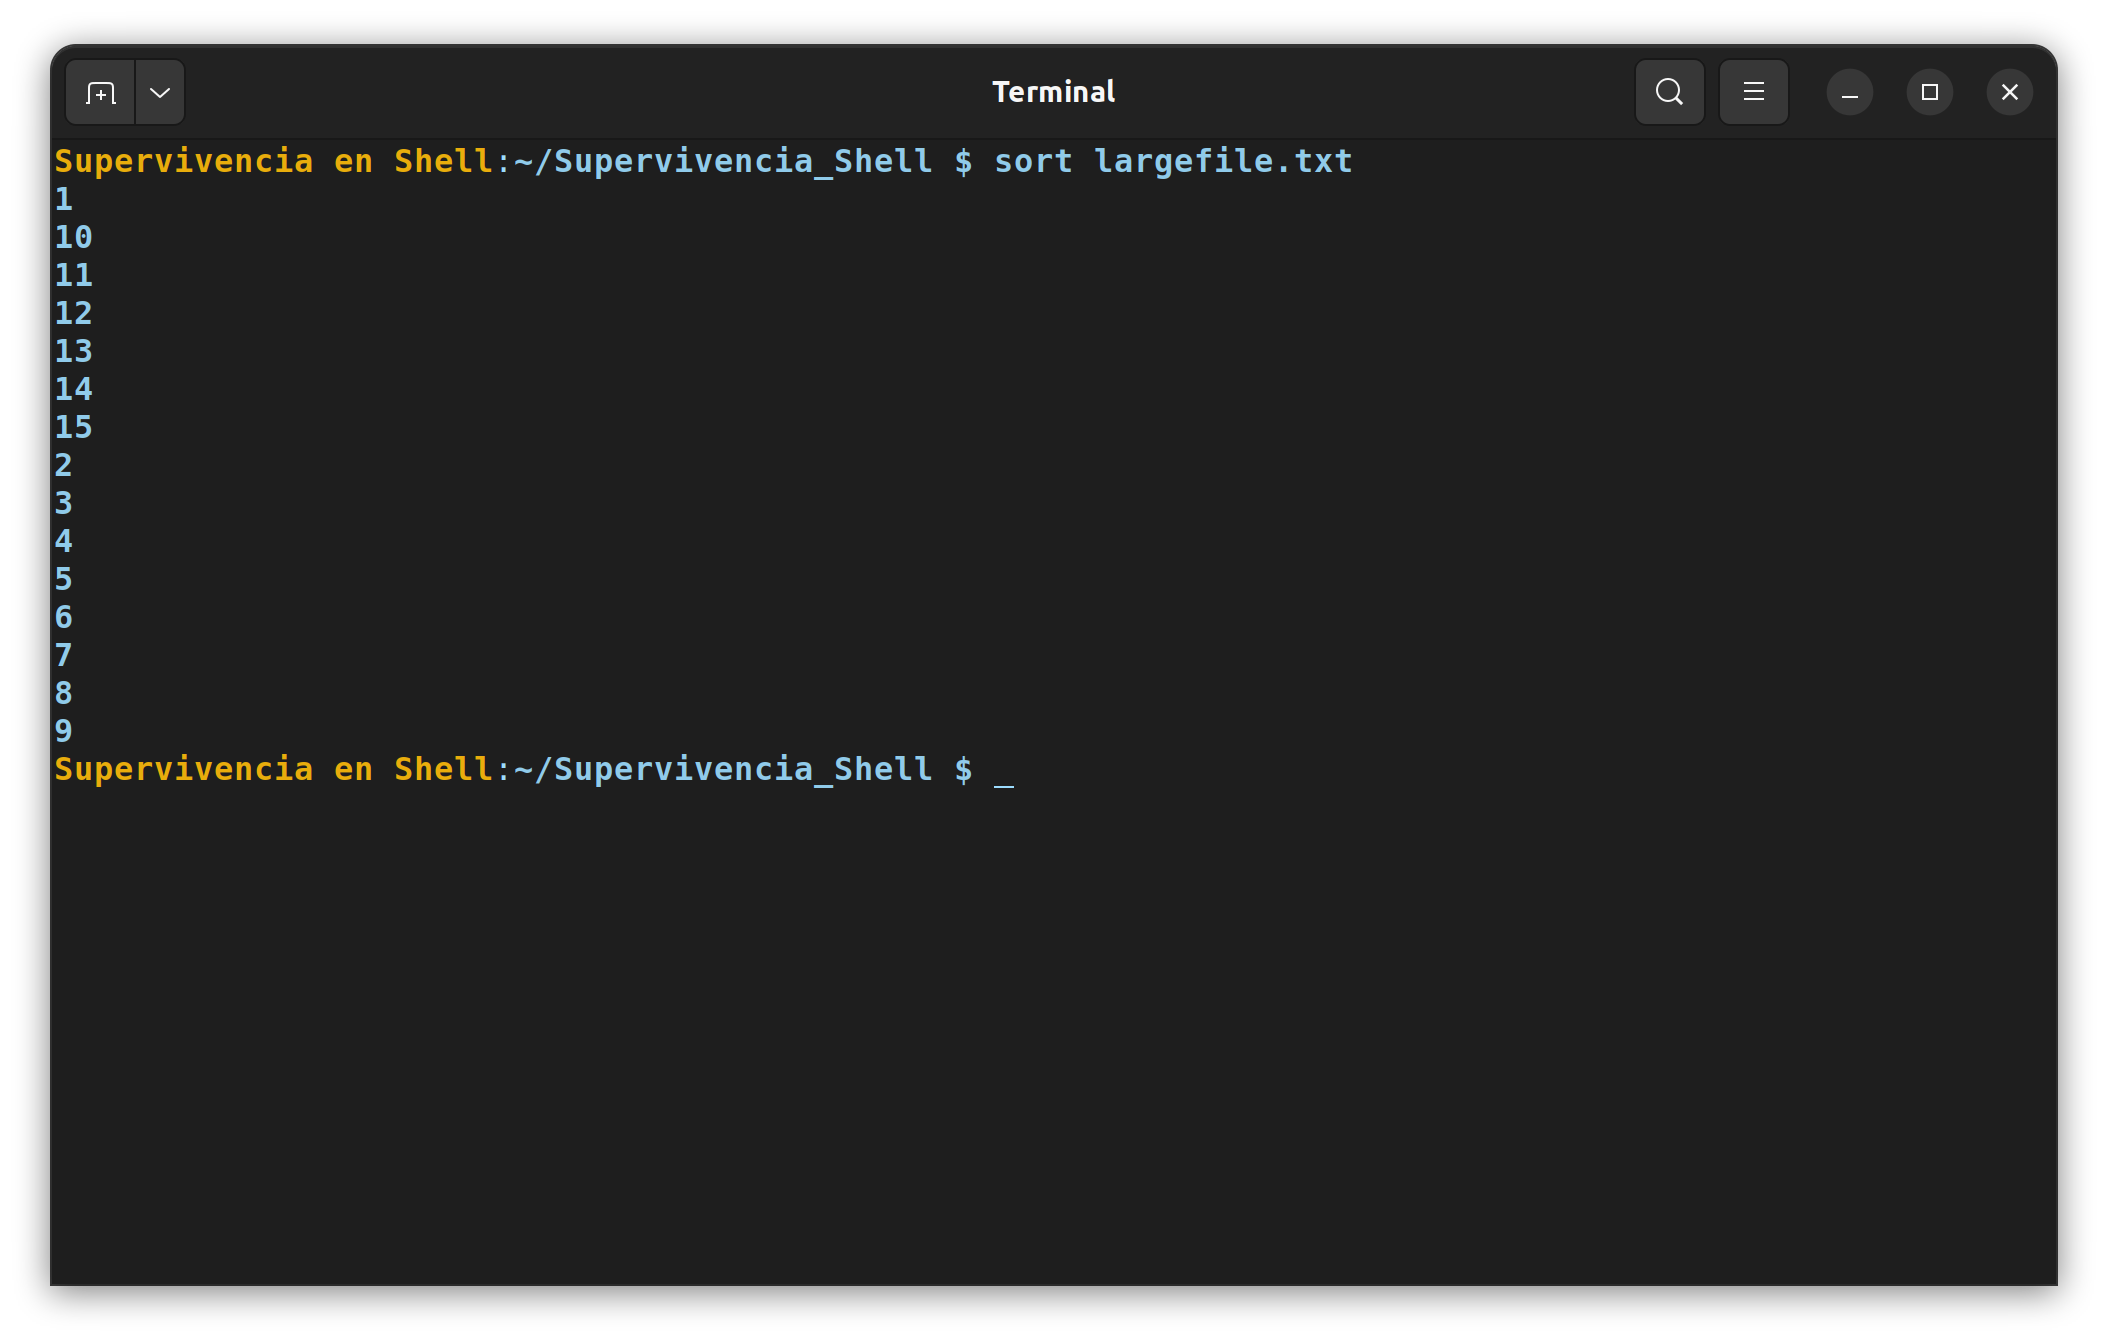
\includegraphics[width=0.55\textwidth]{sort}
		\end{center}
	\end{frame}
		
	\begin{frame}
		\frametitle{Comparando ficheros: cmp}
		\begin{alertblock}{Compara ficheros byte a byte.}
			cmp [OPTION]... FILE1 FILE2
		\end{alertblock}
		\begin{center}
			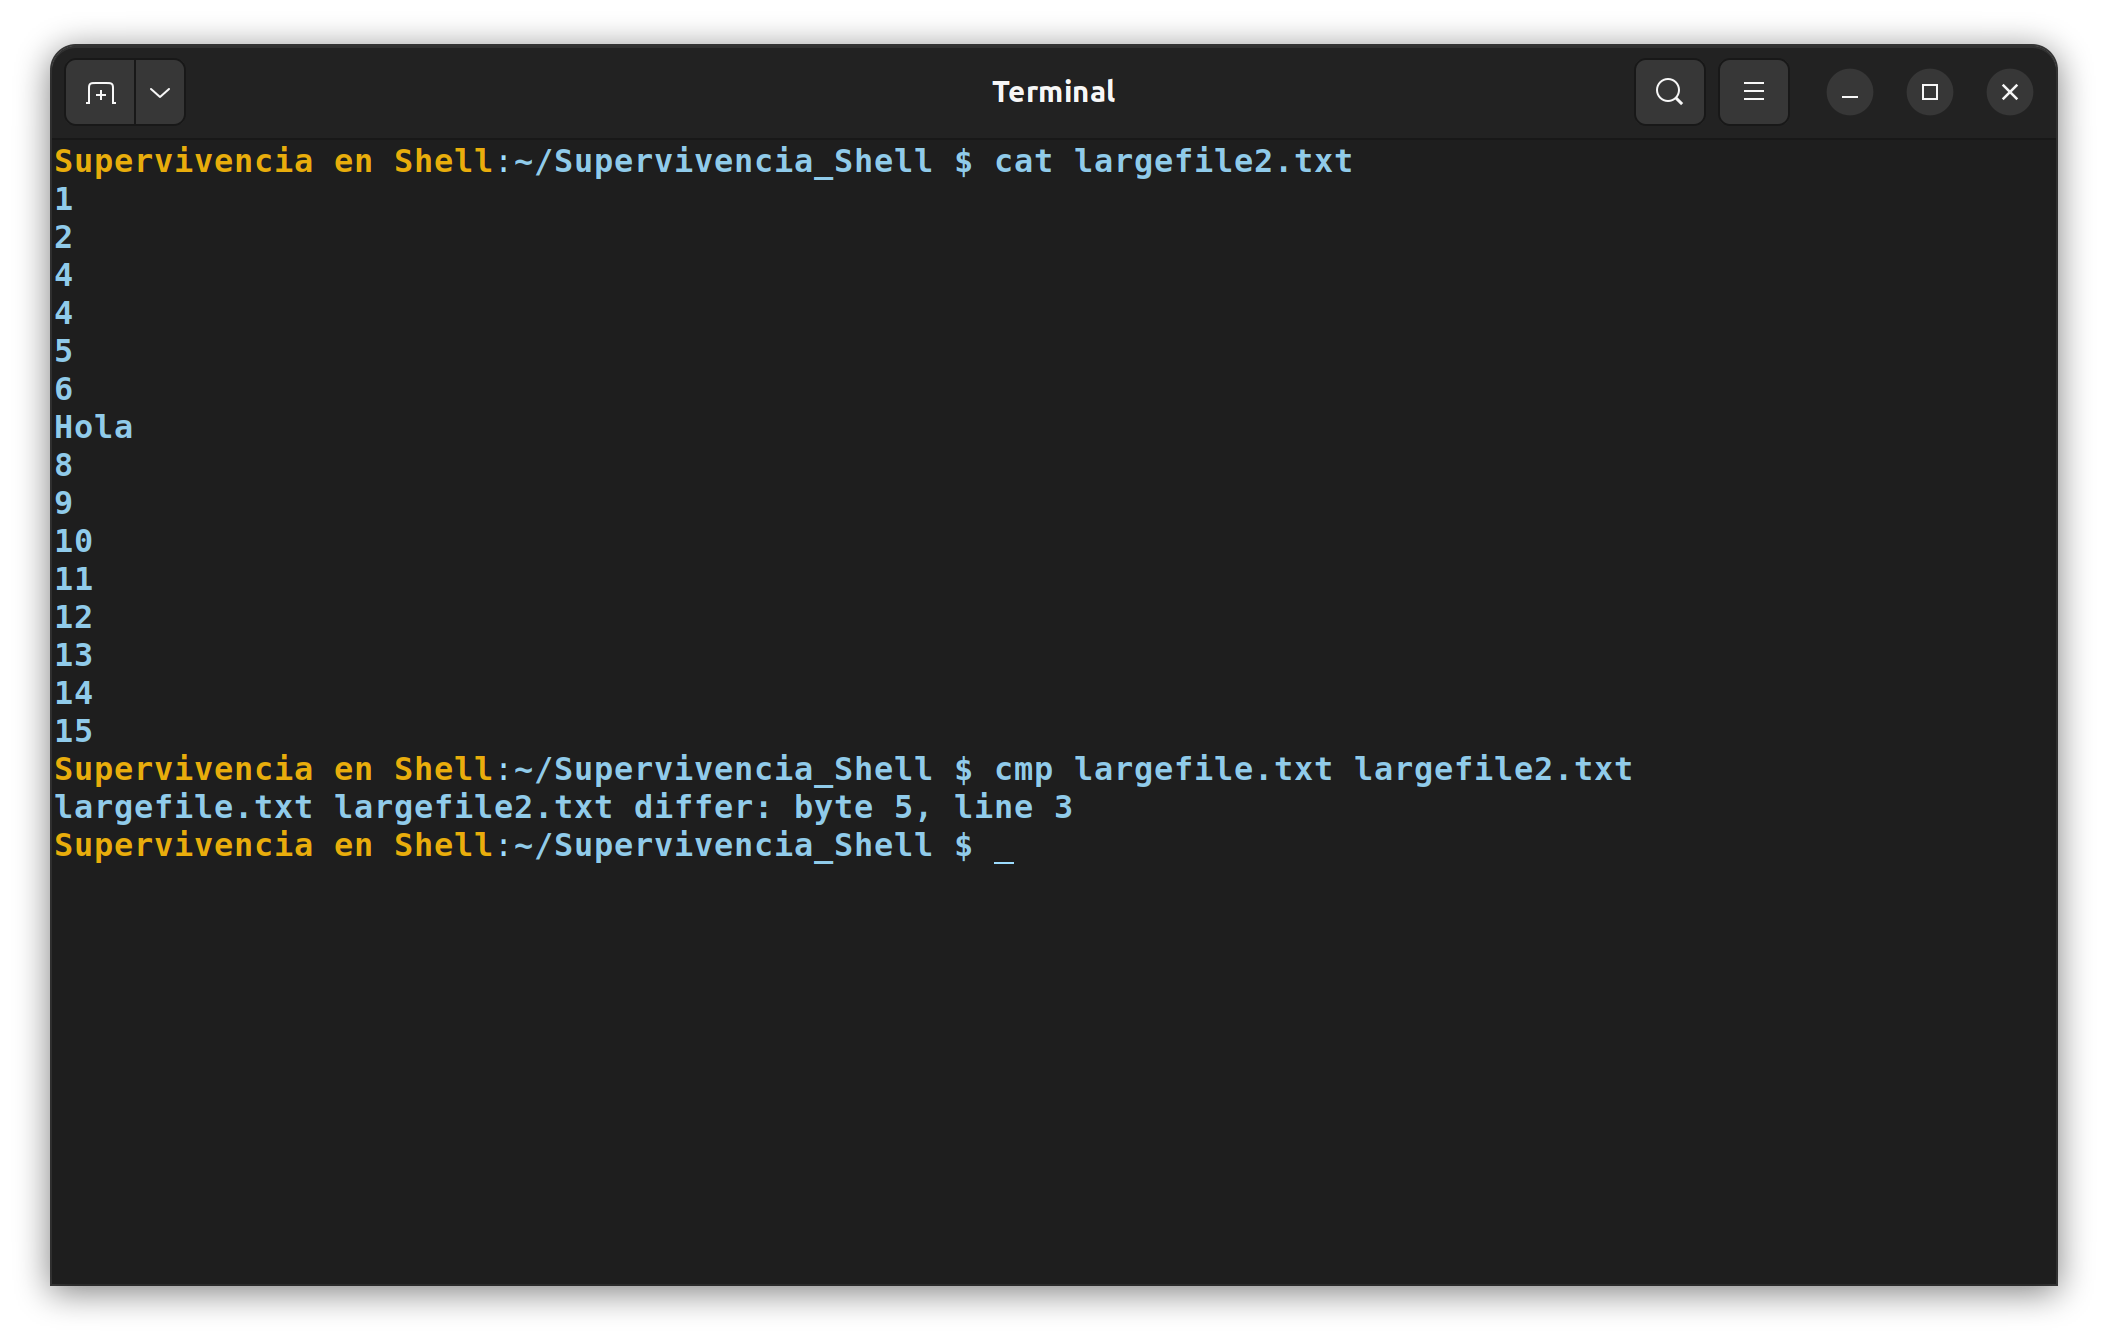
\includegraphics[width=0.55\textwidth]{cmp}
		\end{center}
	\end{frame}
	
	\begin{frame}
		\frametitle{Comparando ficheros: diff}
		\begin{alertblock}{Compara ficheros linea a linea.}
			diff [OPTION]... FILES
		\end{alertblock}
		\begin{center}
			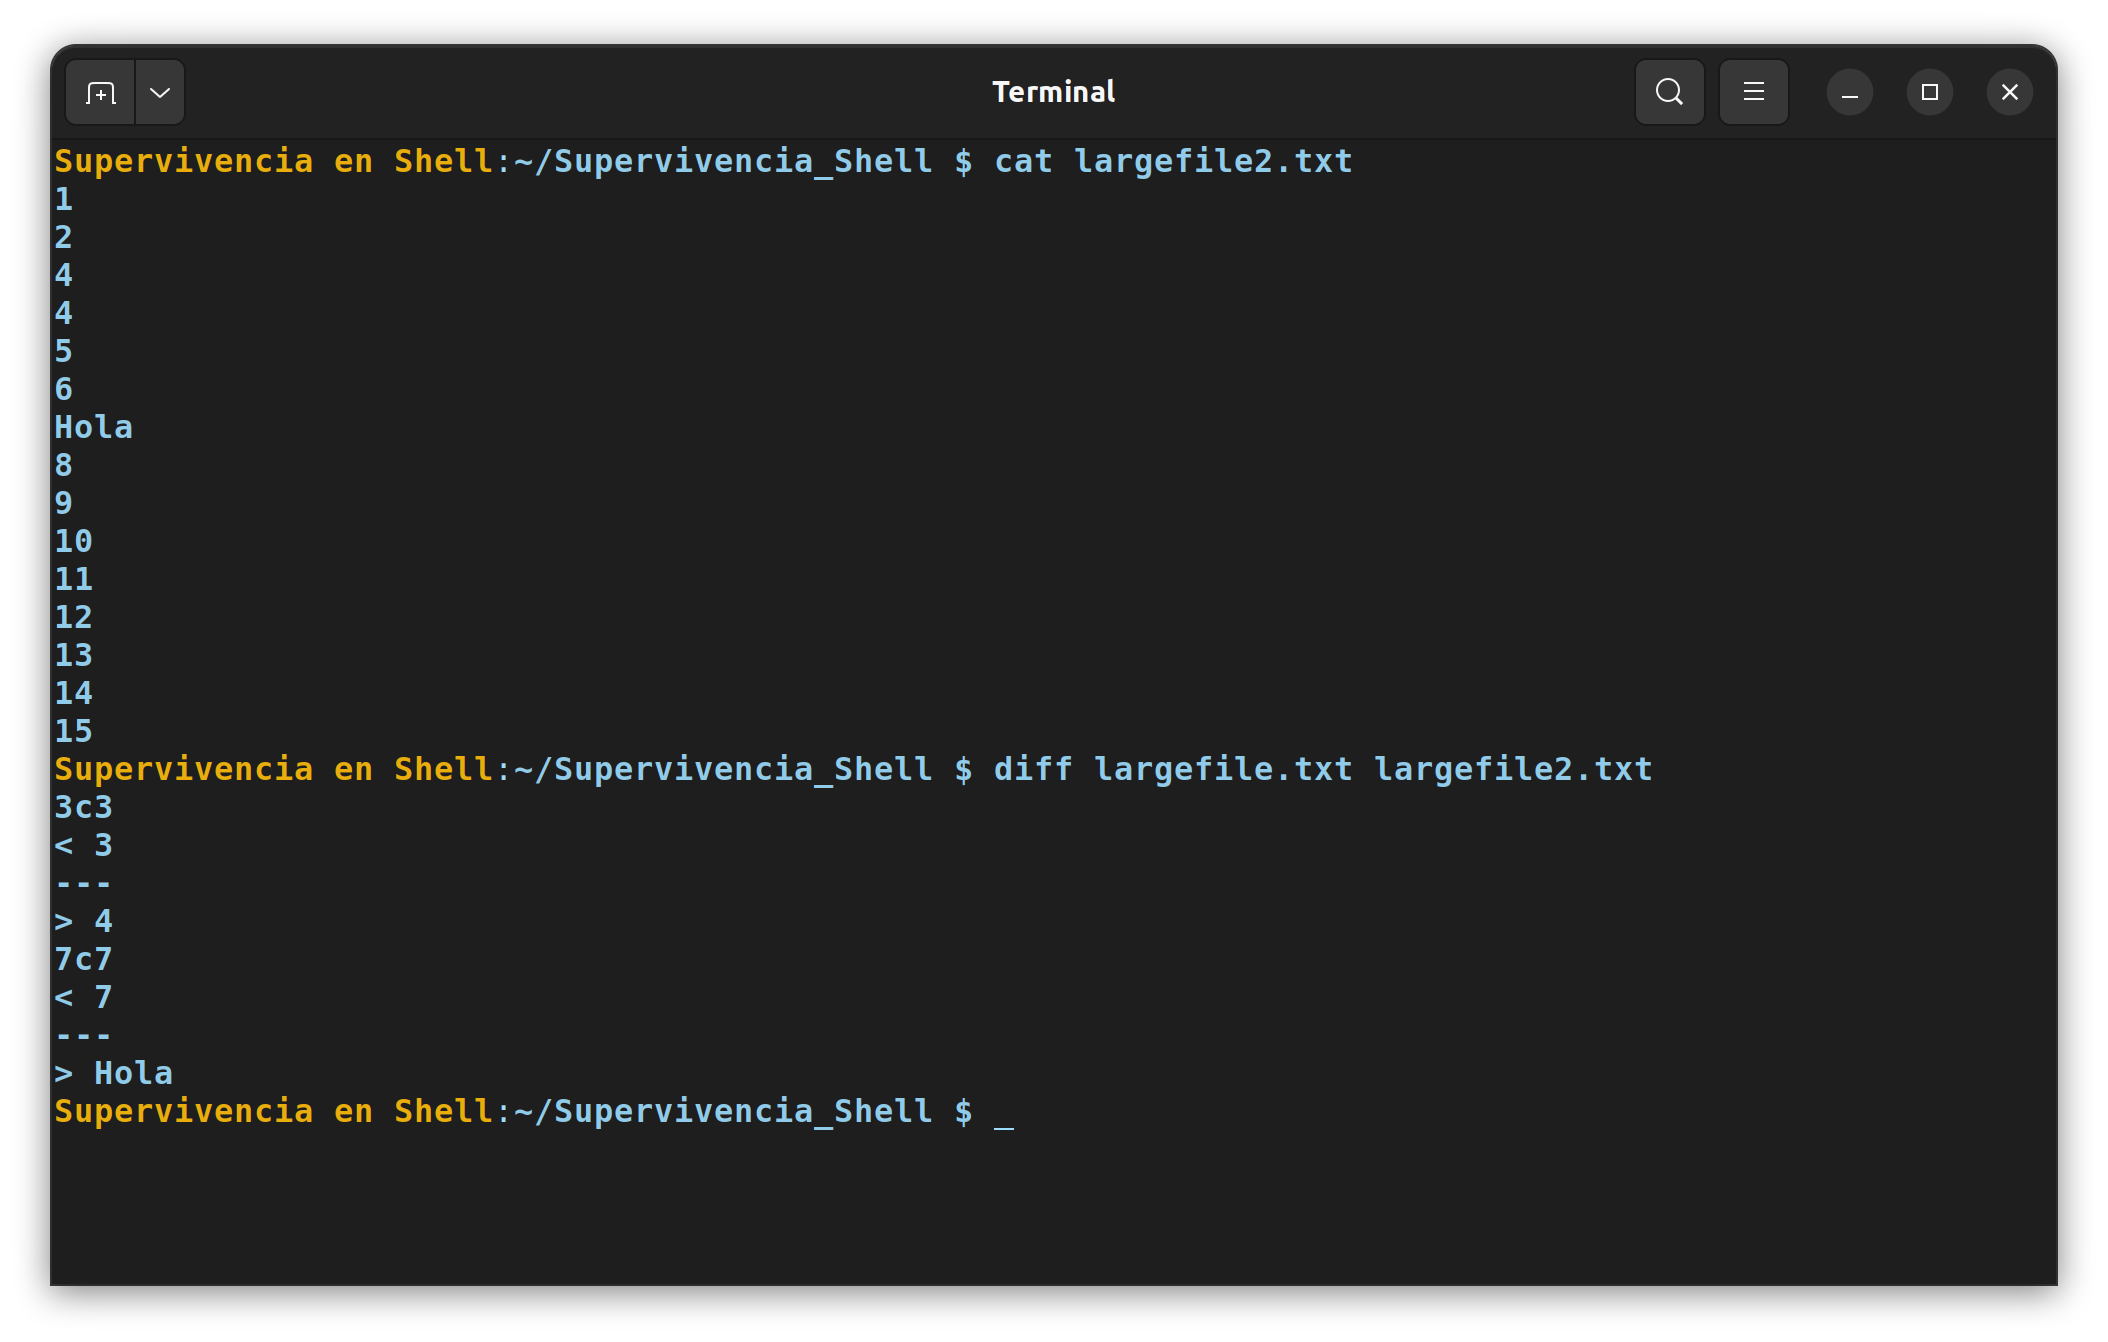
\includegraphics[width=0.55\textwidth]{diff}
		\end{center}
	\end{frame}
			
	\begin{frame}
		\frametitle{Modificando ficheros: tar (Flags)}
		\begin{alertblock}{Crea un fichero con múltiples ficheros dentro (comprimidos o no).}
			tar -czvf [ARCHIVE] [SOURCE]
		\end{alertblock}
		Los flags significan:
		\begin{itemize}
			\item -c: crea un nuevo archivo.
			\item -z: comprime usando gzip.
			\item -v: \textbf{opcional}, lista los ficheros procesados.
			\item -f: \textbf{siempre el último}, y significa que usa el fichero ARCHIVE.
		\end{itemize}
	\end{frame}
	
	\begin{frame}
		\frametitle{Modificando ficheros: tar}
		\begin{alertblock}{Crea un fichero con múltiples ficheros dentro (comprimidos o no).}
			tar -czvf [ARCHIVE] [SOURCE]
		\end{alertblock}
		\begin{center}
			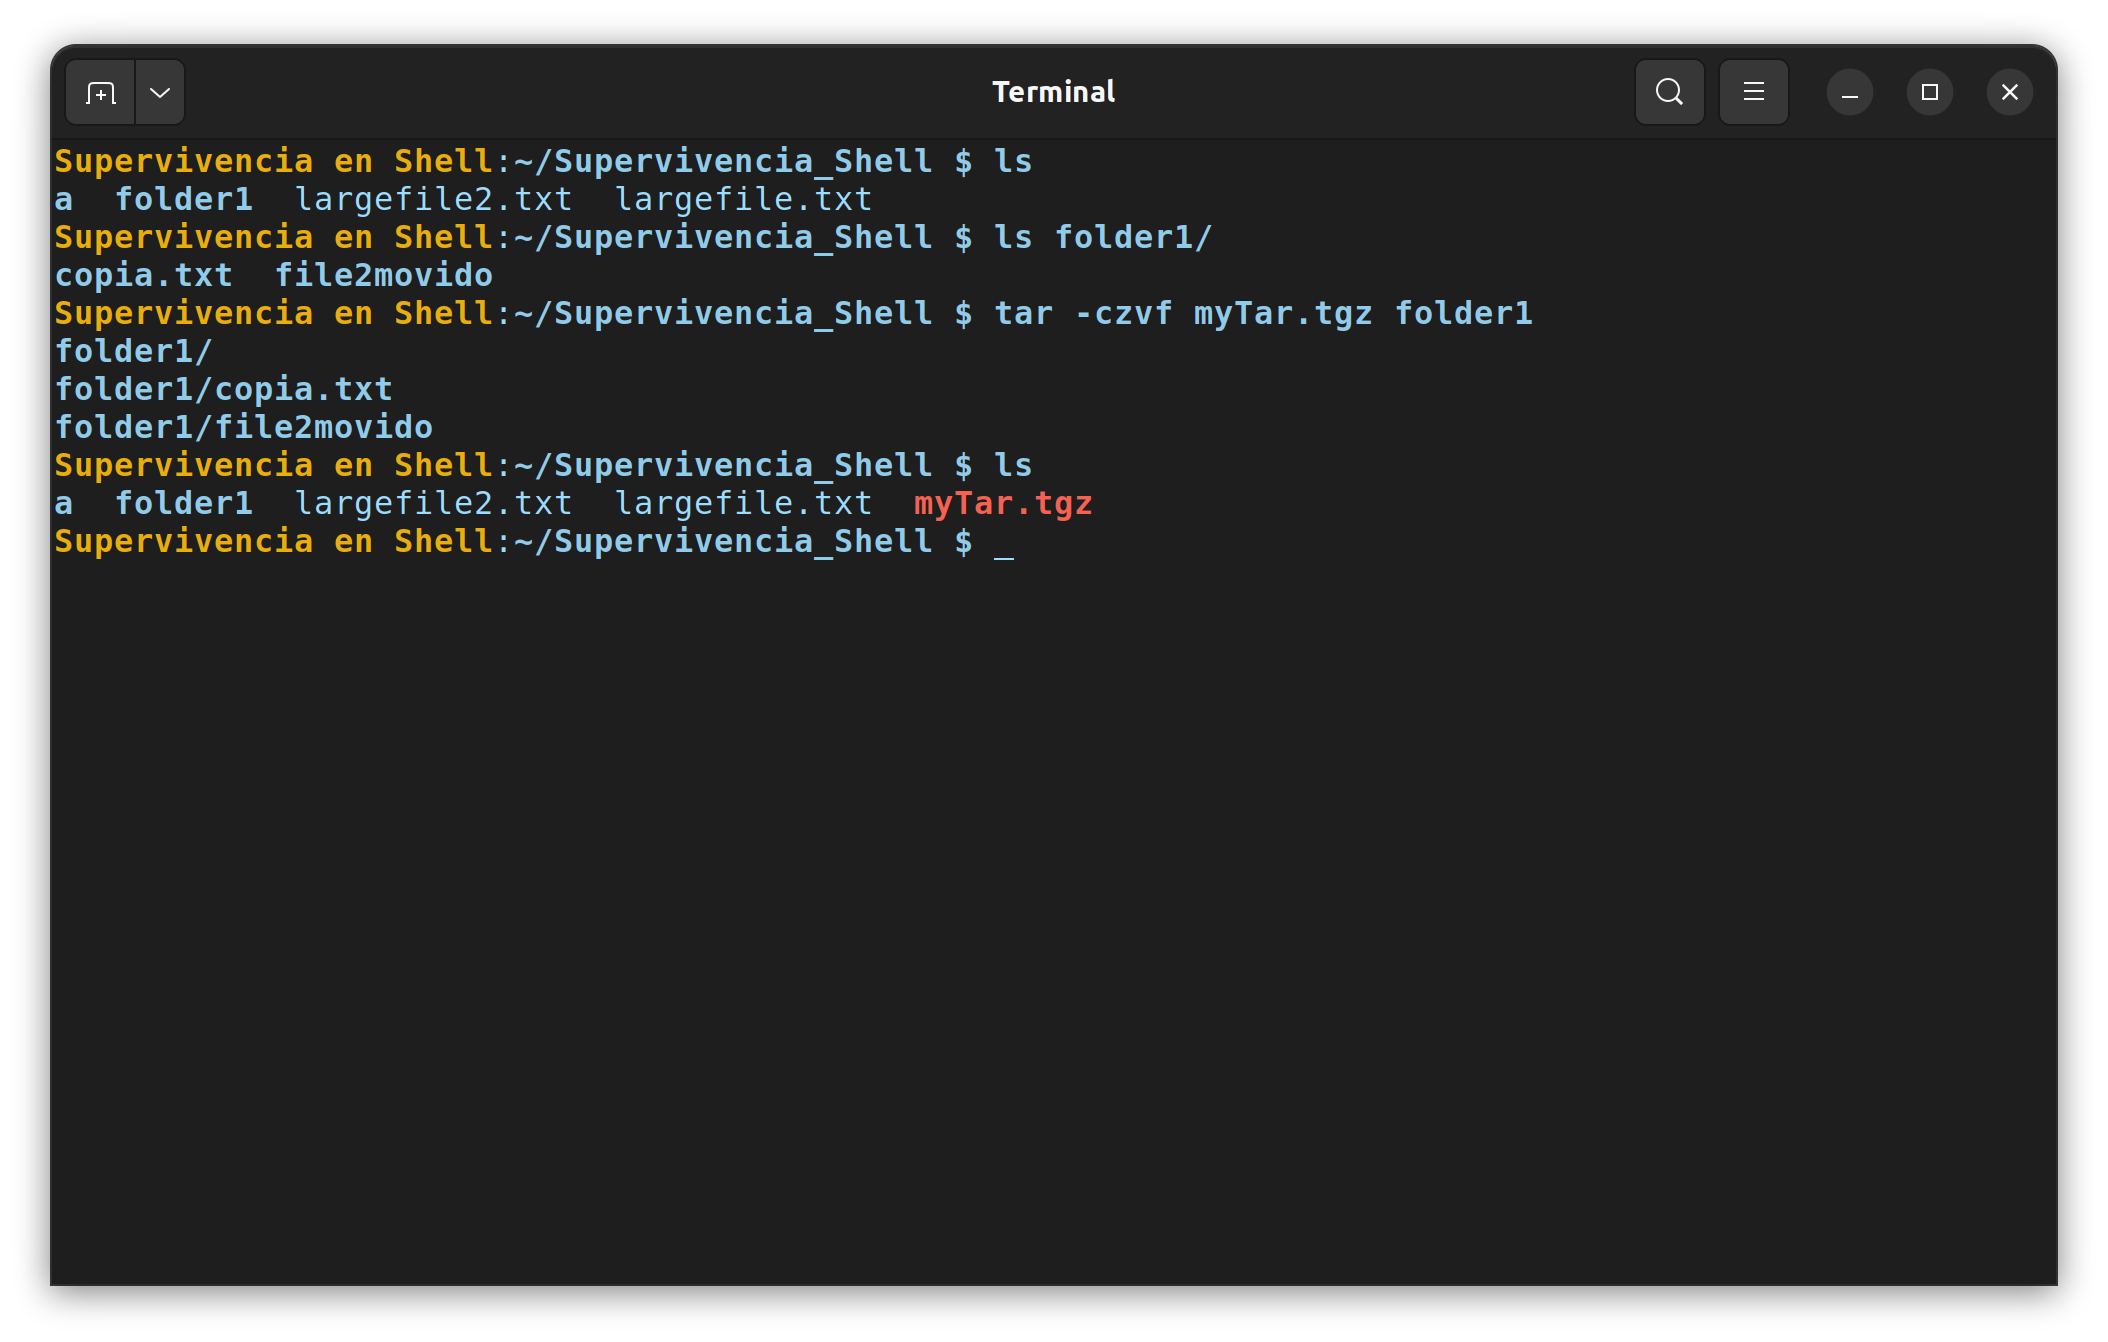
\includegraphics[width=0.55\textwidth]{tar}
		\end{center}
	\end{frame}
	
	\begin{frame}
		\frametitle{Modificando ficheros: gzip/gunzip}
		\begin{alertblock}{Comprime/descomprime un fichero.}
			gzip/gunzip [OPTION]... [FILE]
		\end{alertblock}
		\begin{center}
			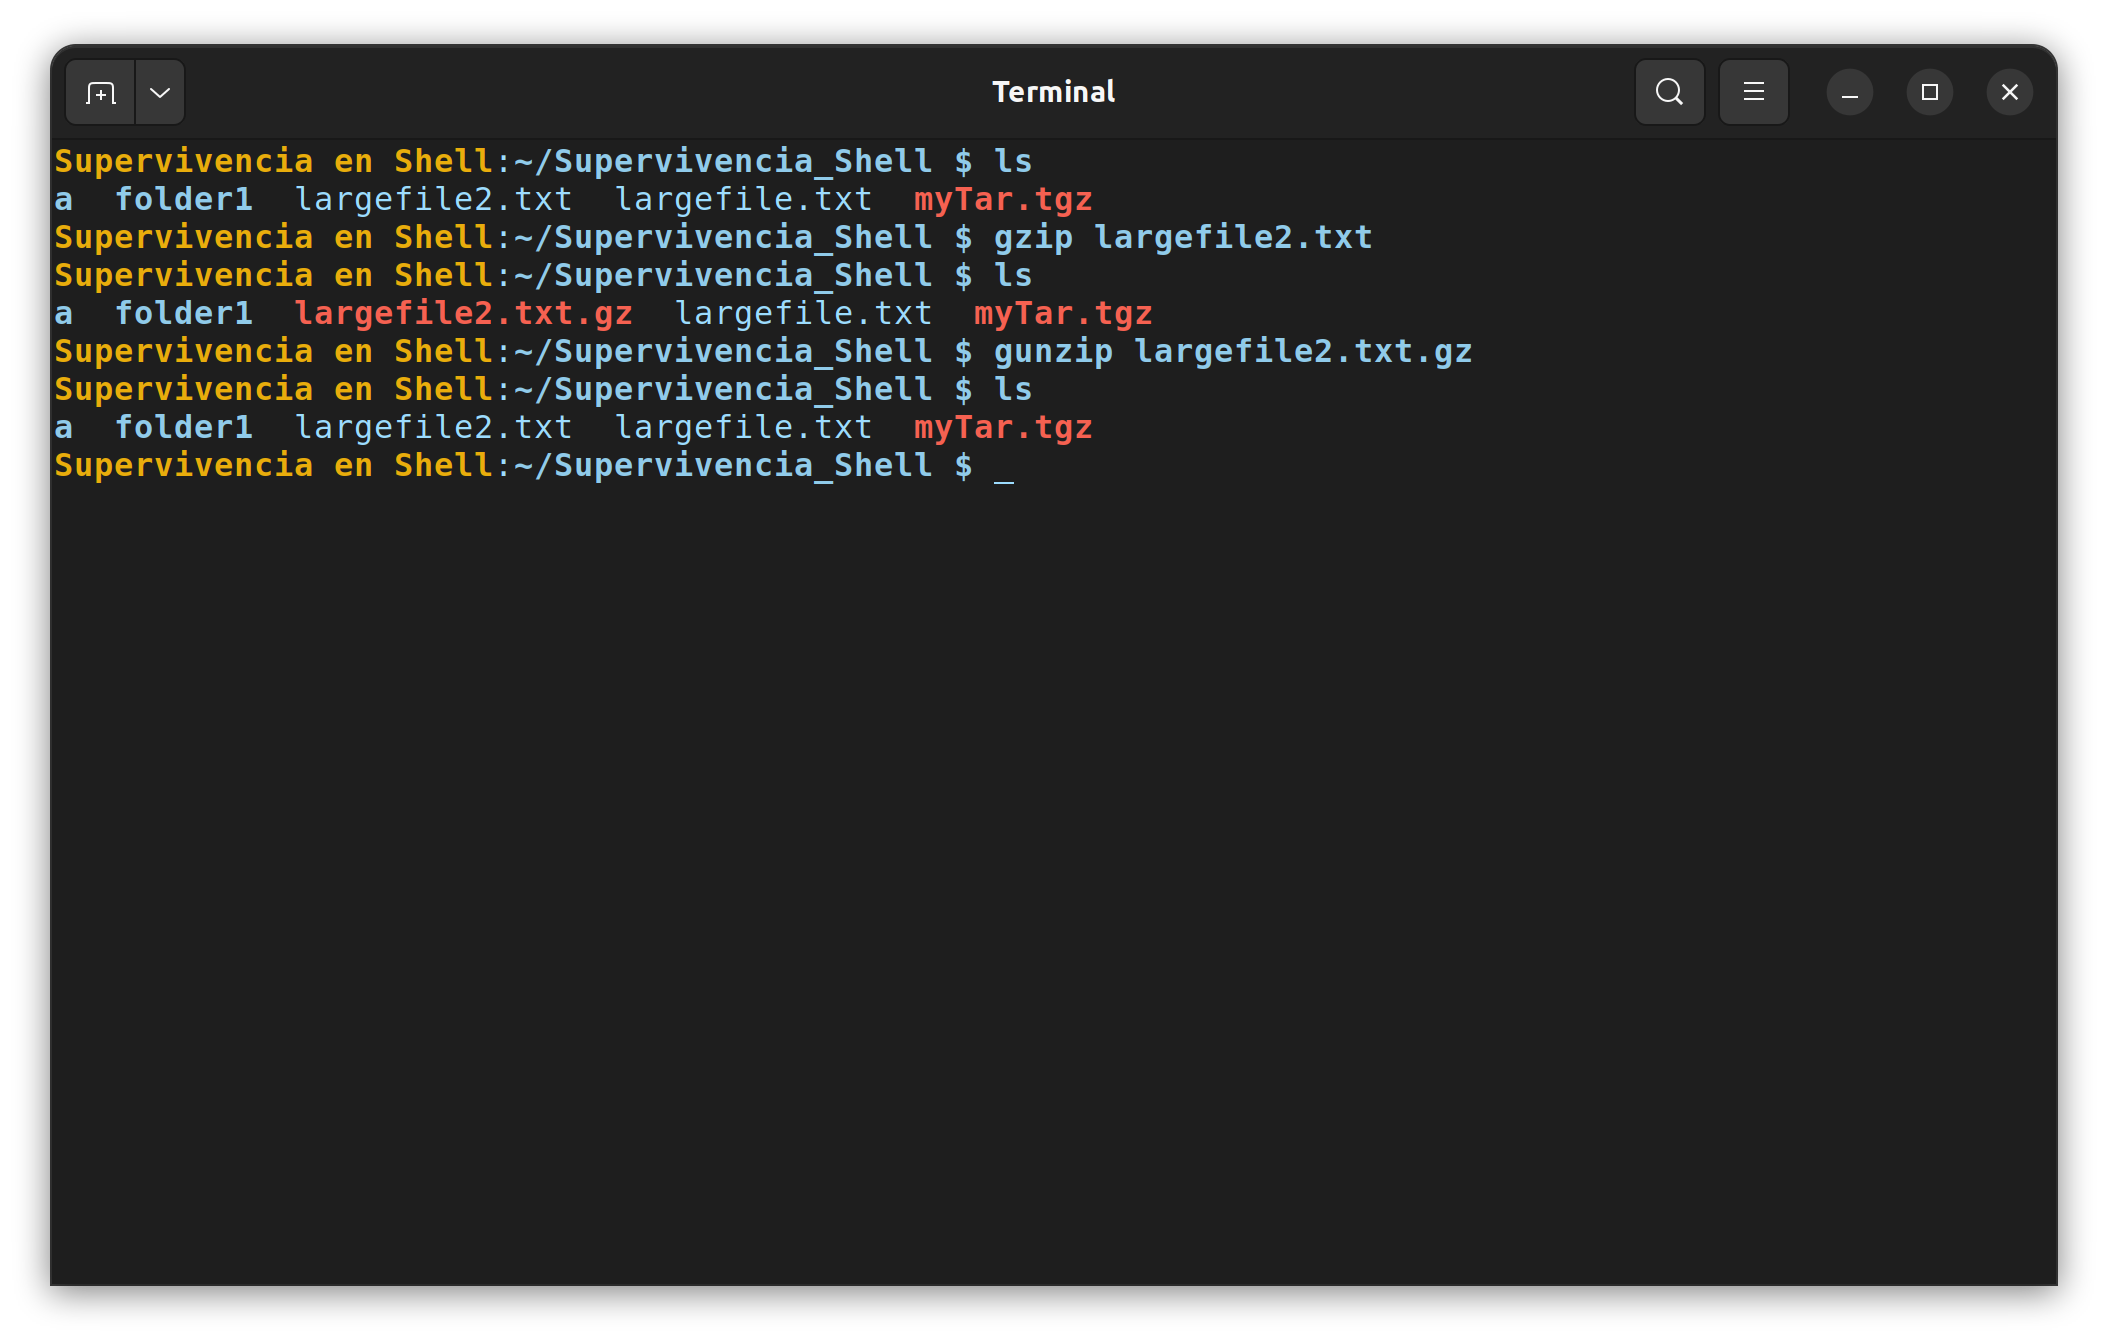
\includegraphics[width=0.55\textwidth]{gzip}
		\end{center}
	\end{frame}
		
	\begin{frame}
		\frametitle{Modificando ficheros: nano}
		\begin{alertblock}{Editor de texto.}
			nano [FILE]...
		\end{alertblock}
		\begin{center}
			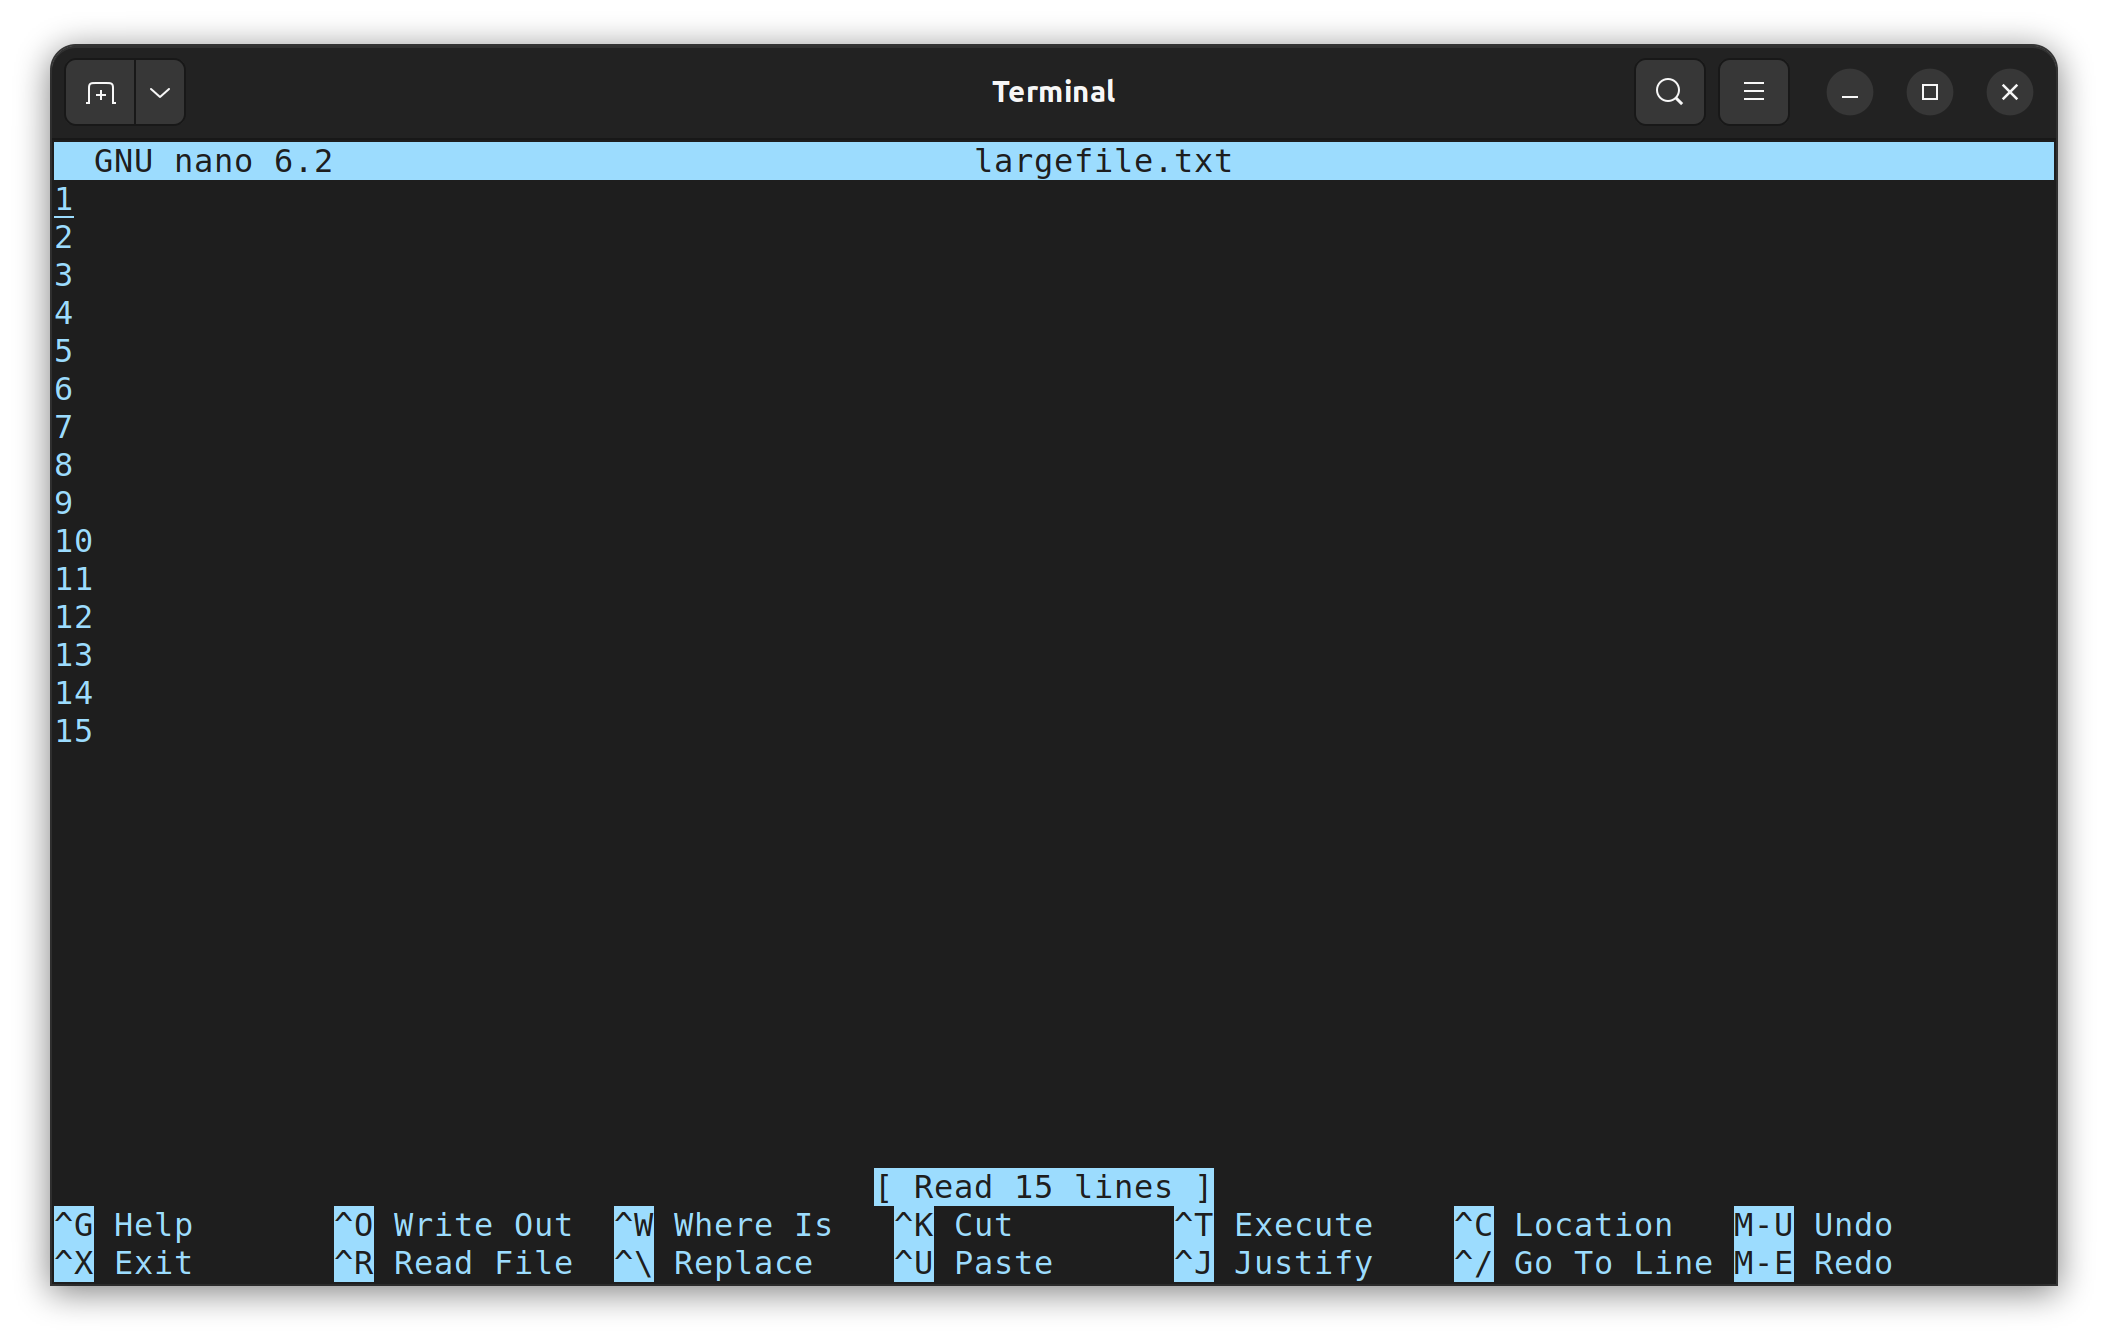
\includegraphics[width=0.55\textwidth]{nano}
		\end{center}
	\end{frame}
	
	\begin{frame}
		\frametitle{Modificando ficheros: vi/vim}
		\begin{alertblock}{Editor de texto. Importante: se sale con Esc y :q!.}
			vi/vim [options] [file ..]
		\end{alertblock}
		\begin{center}
			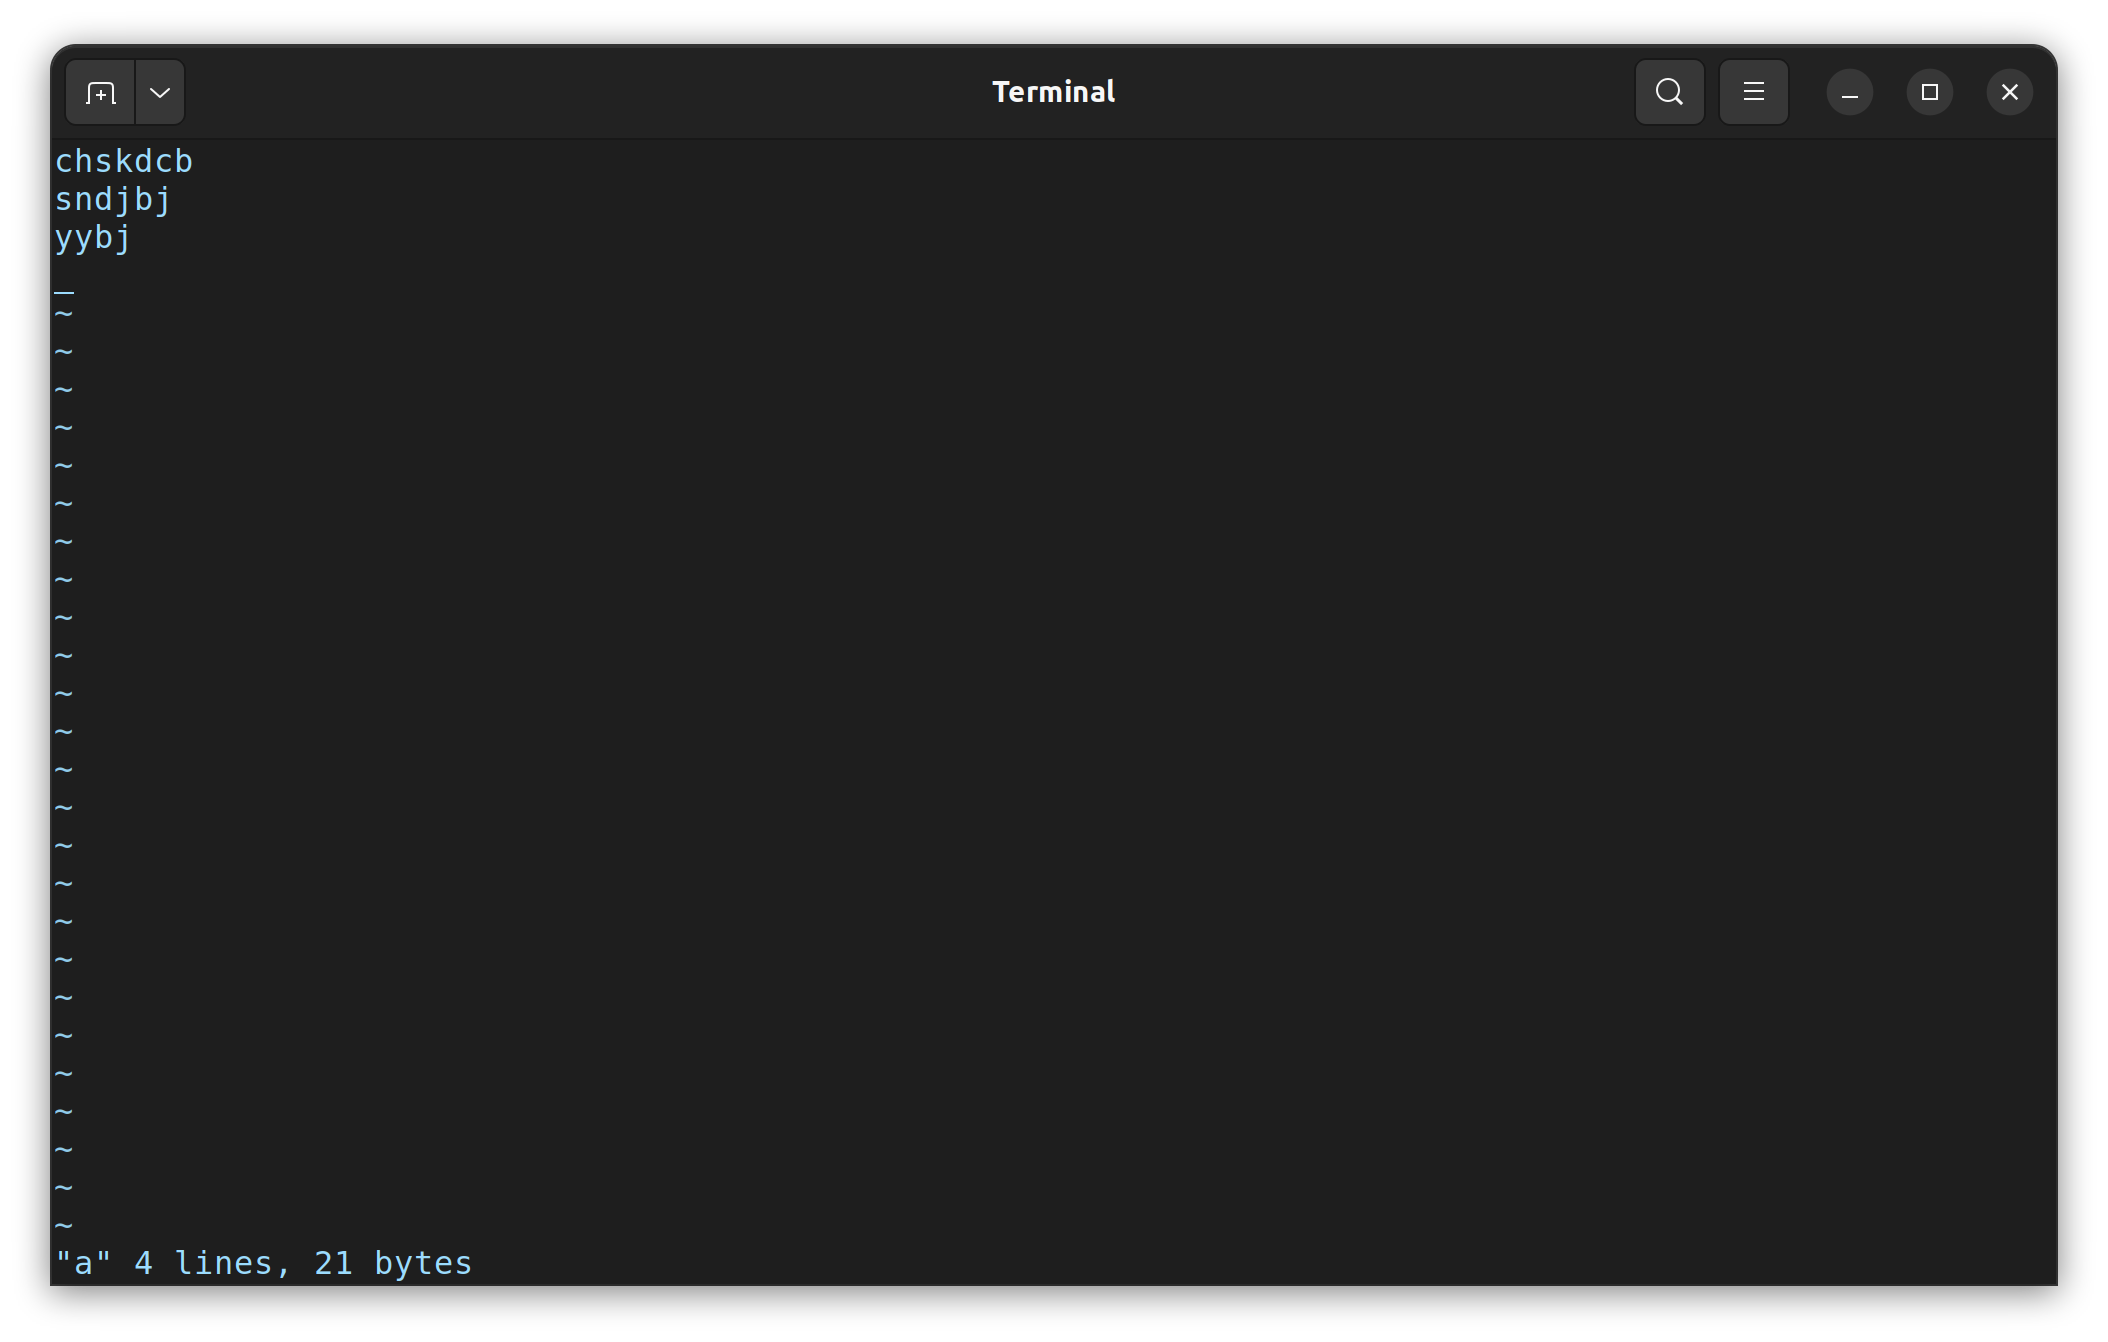
\includegraphics[width=0.55\textwidth]{vim}
		\end{center}
	\end{frame}
	
	\begin{frame}
		\frametitle{Controlando el terminal: clear}
		\begin{alertblock}{Limpia el terminal.}
			clear
		\end{alertblock}
		\begin{center}
			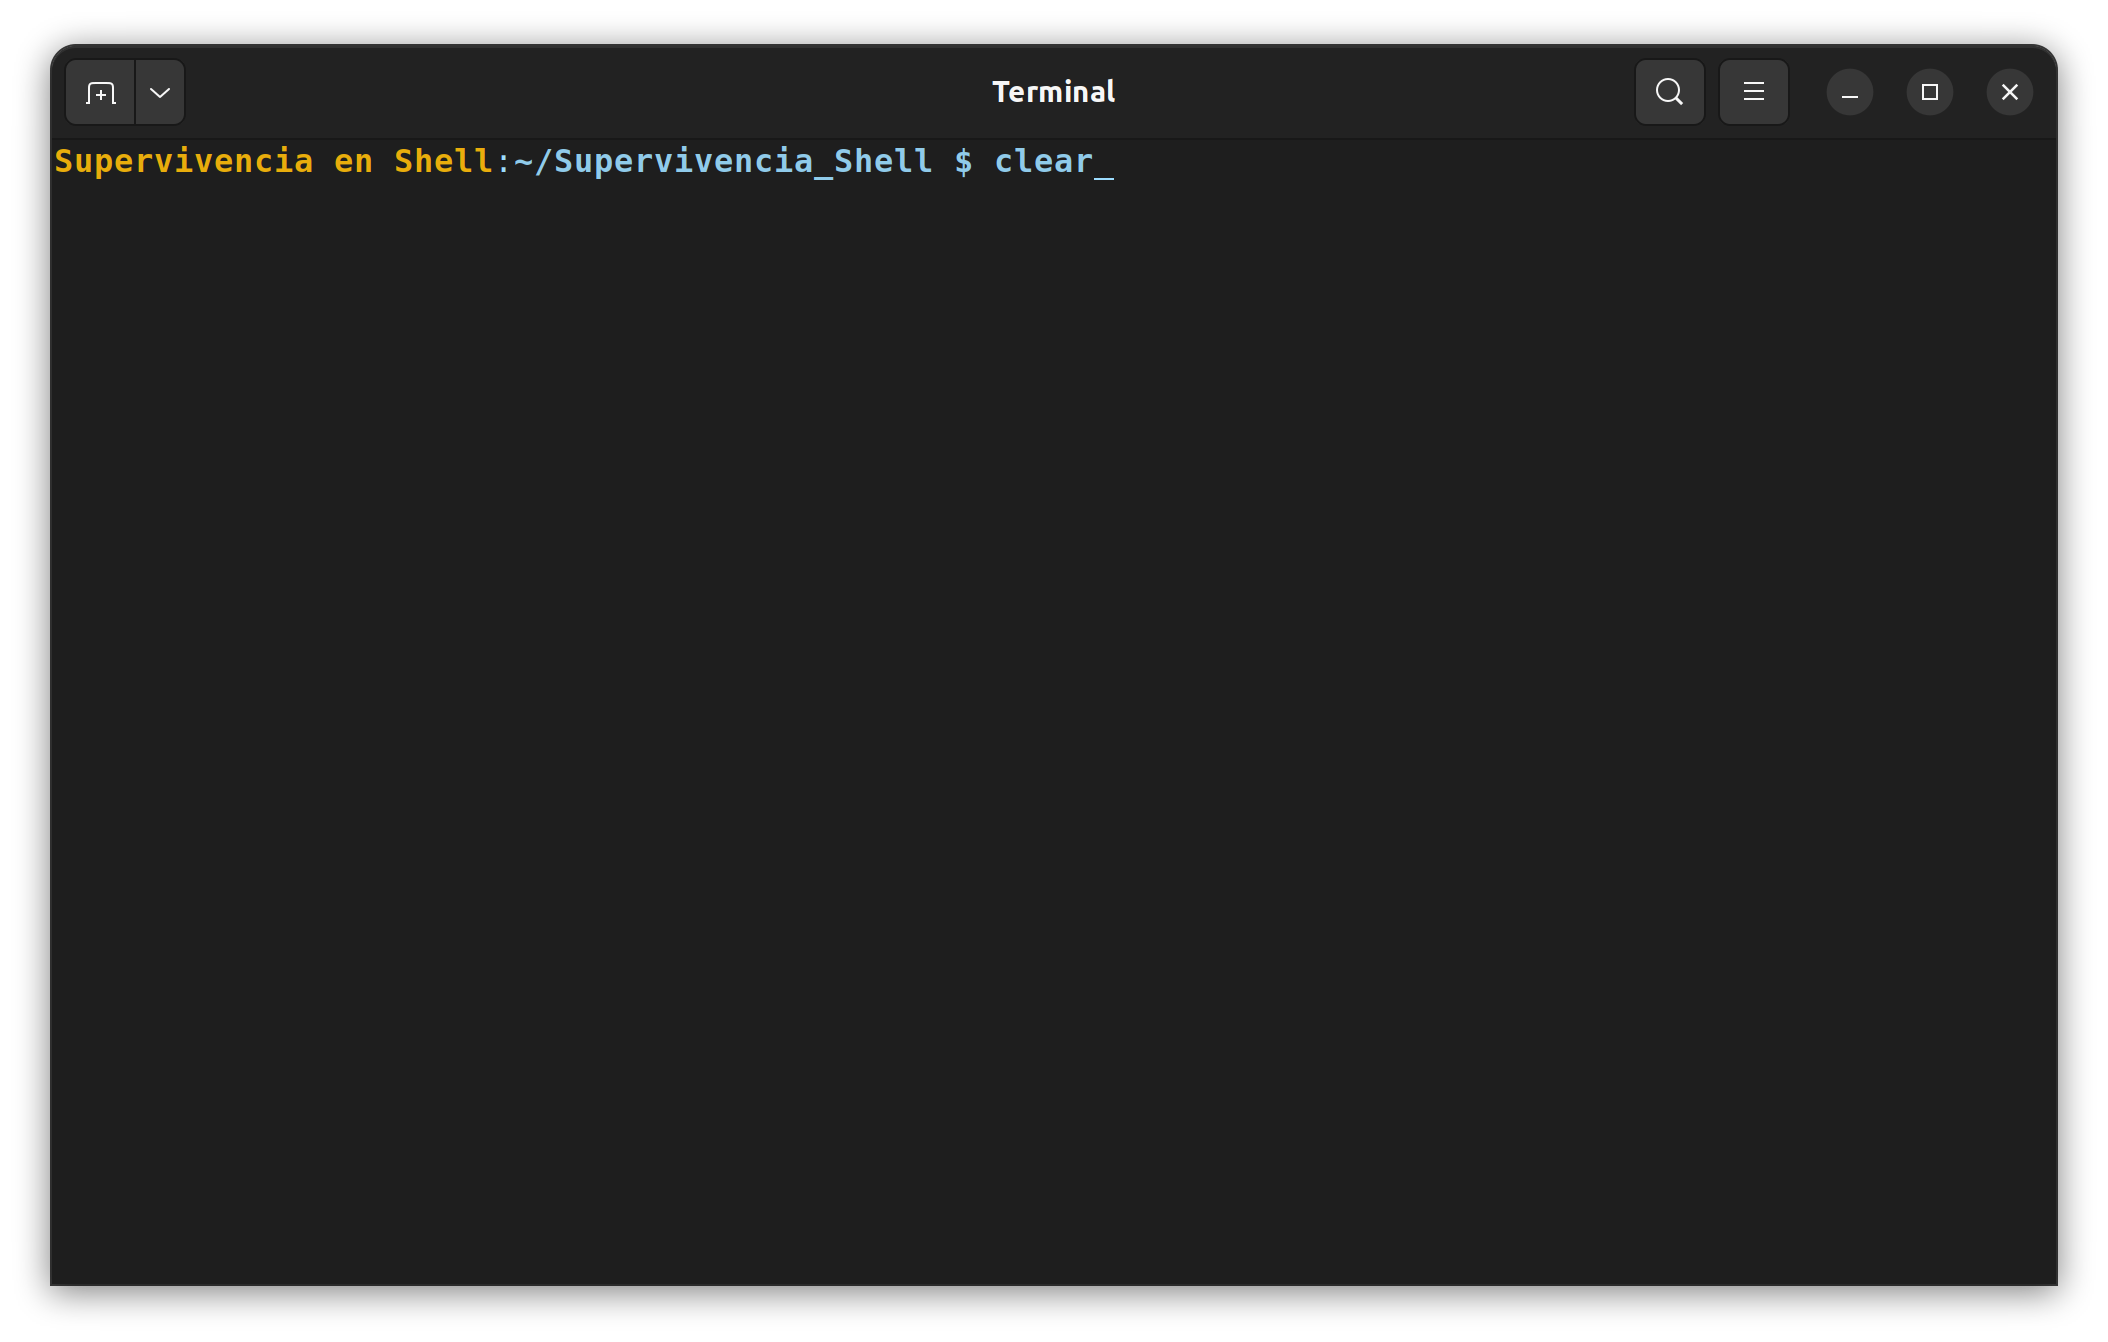
\includegraphics[width=0.55\textwidth]{clear}
		\end{center}

	\end{frame}	
	
	\begin{frame}
		\frametitle{Controlando el terminal: reset}
		\begin{alertblock}{Reinicia el terminal.}
			reset
		\end{alertblock}
		\begin{center}
			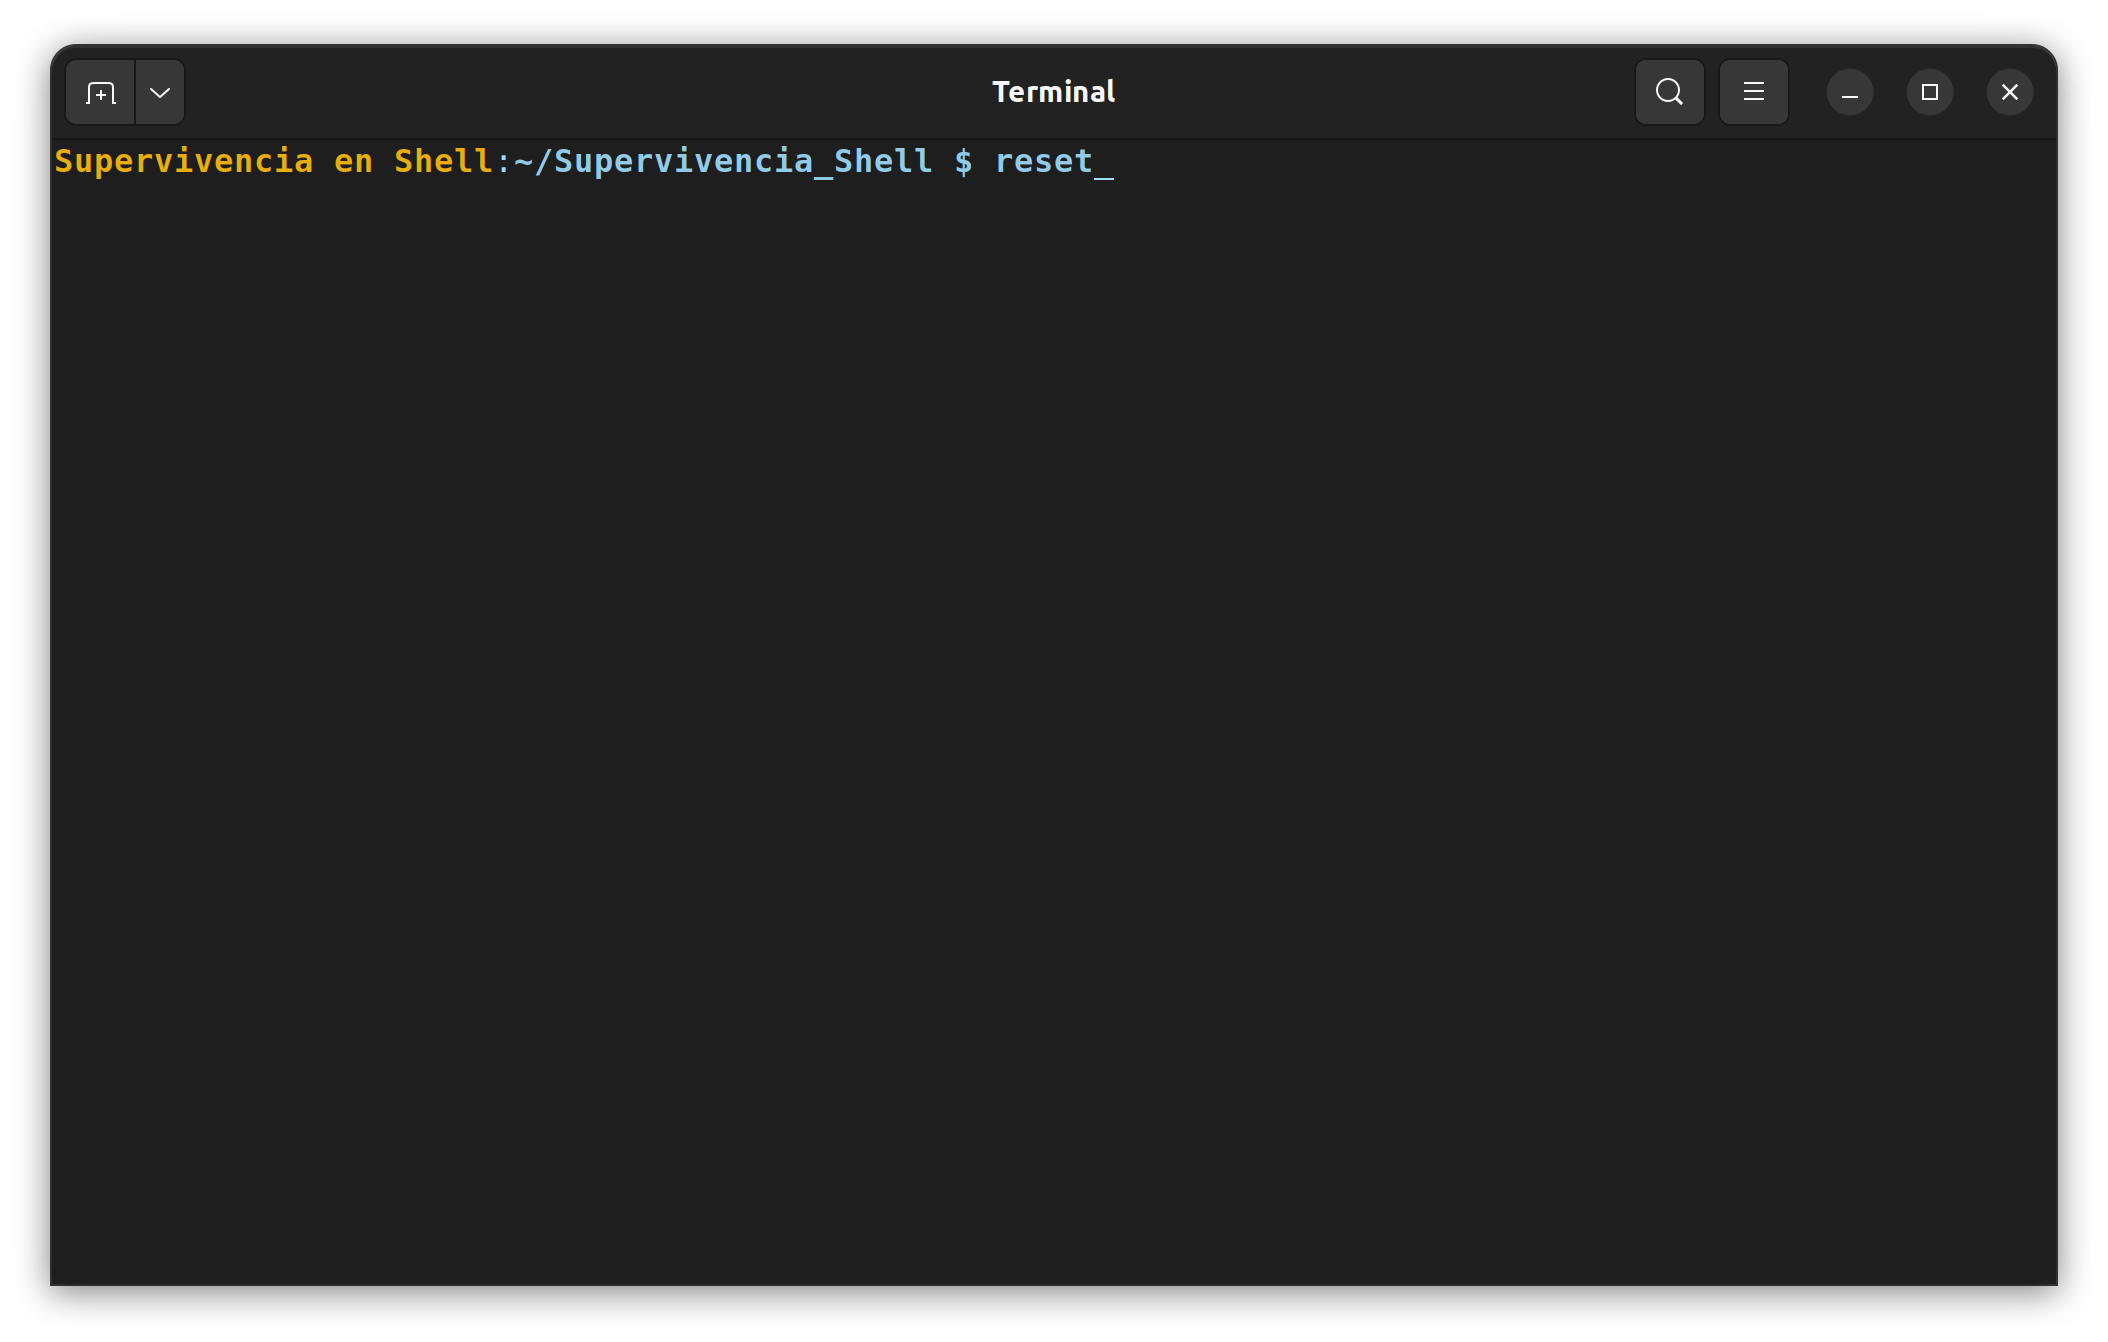
\includegraphics[width=0.55\textwidth]{reset}
		\end{center}
	\end{frame}	
	
	\begin{frame}
		\frametitle{Controlando el terminal: exit}
		\begin{alertblock}{Cierra el terminal.}
			exit
		\end{alertblock}
		\begin{center}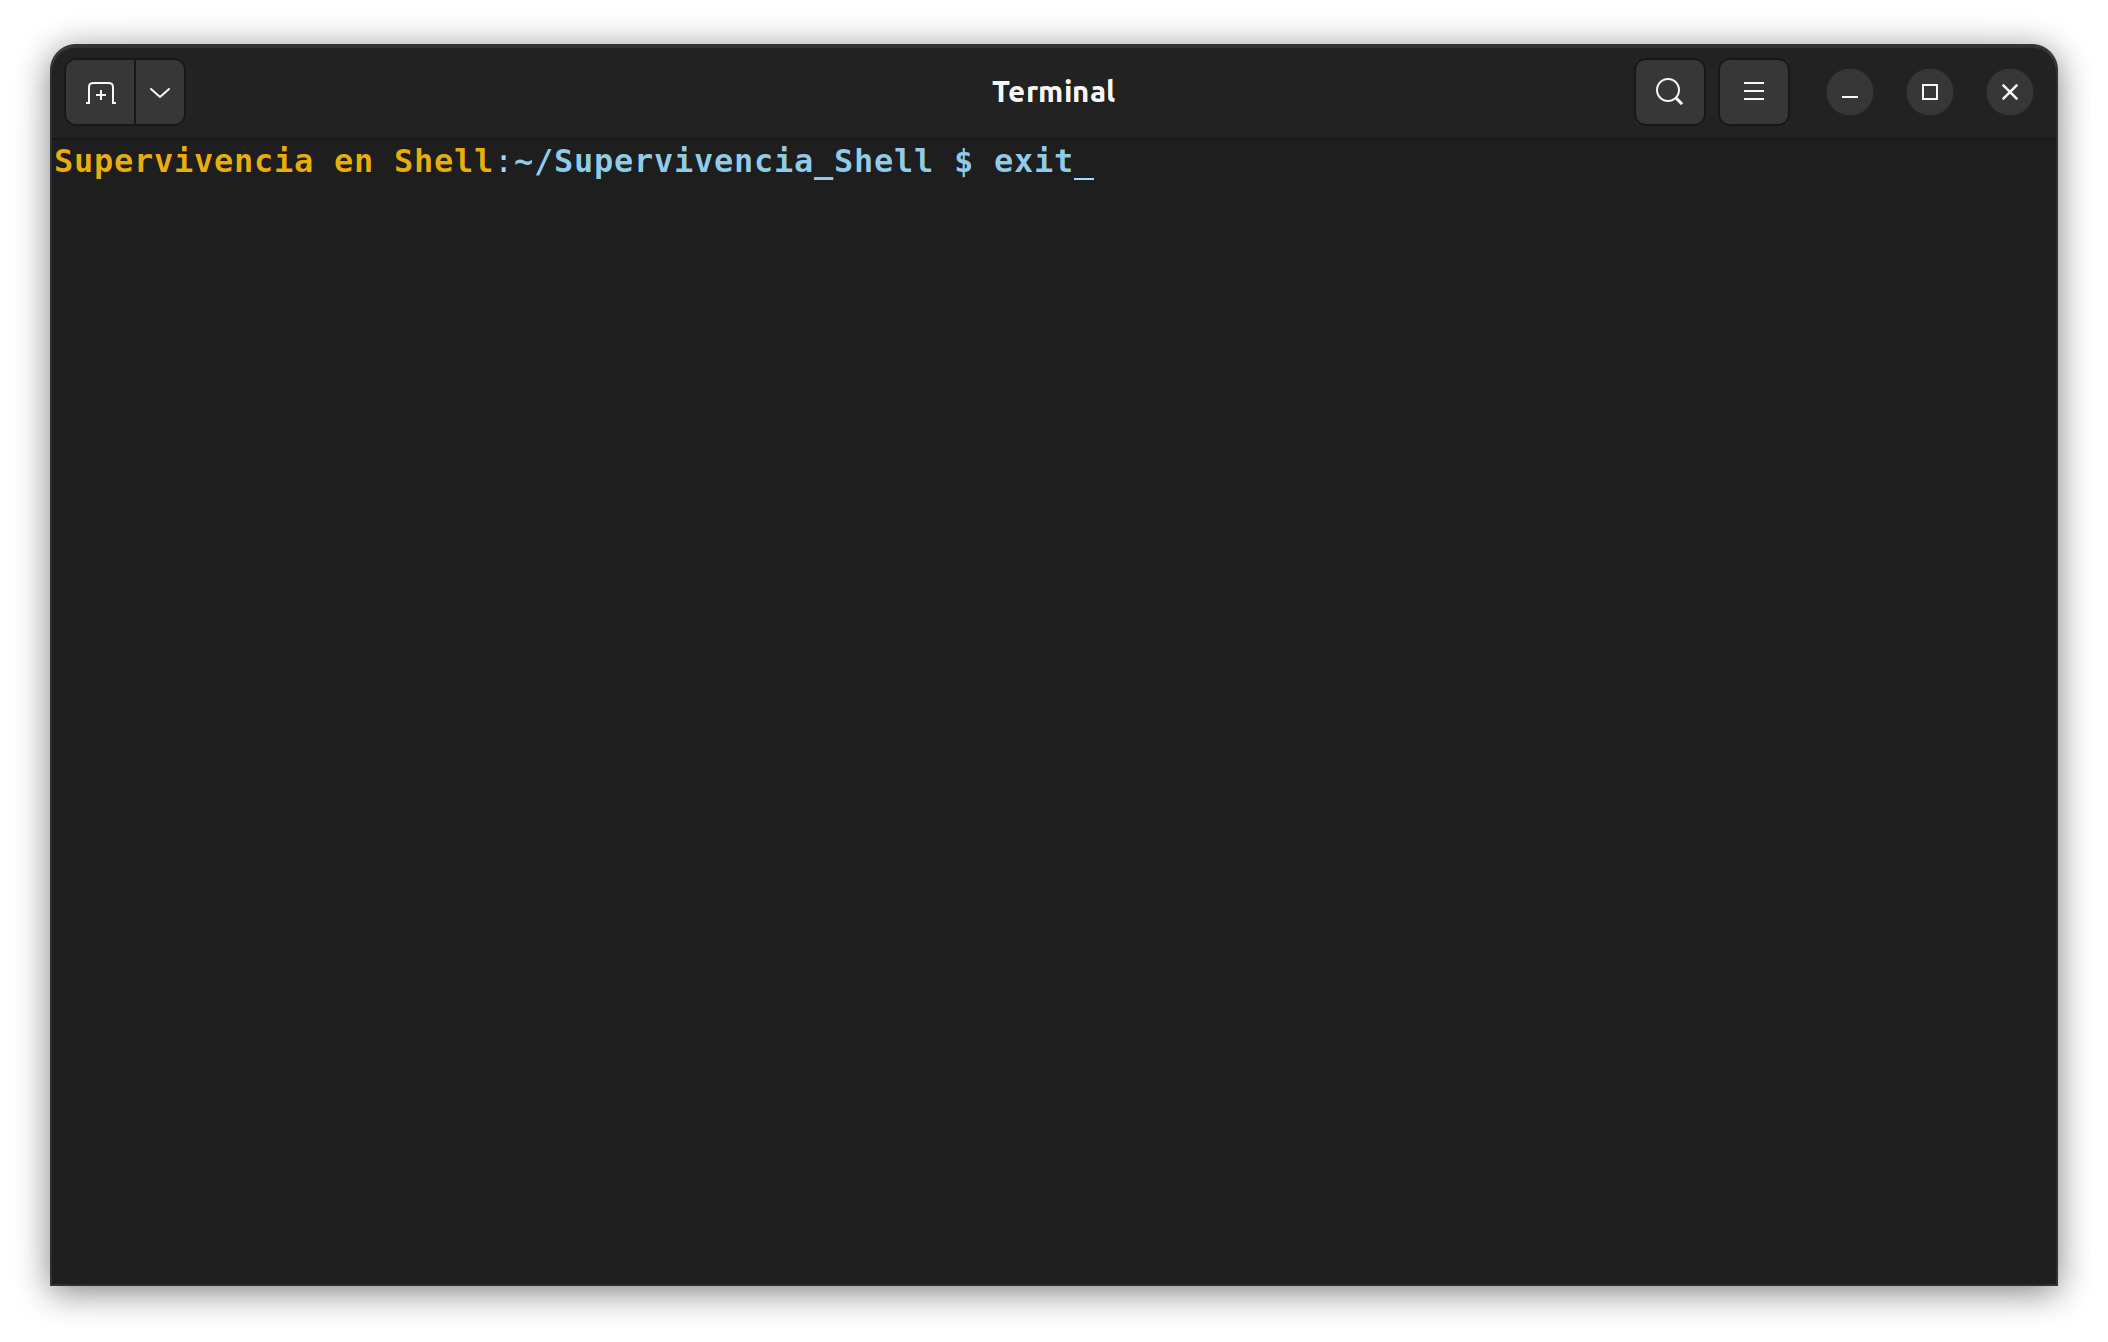
\includegraphics[width=0.55\textwidth]{exit}
		\end{center}
	\end{frame}

	\begin{frame}
		\frametitle{Uso avanzado: alias}
		\begin{alertblock}{Crea un "atajo" para un comando.}
			alias nombre='comando'
		\end{alertblock}
		\begin{center}
			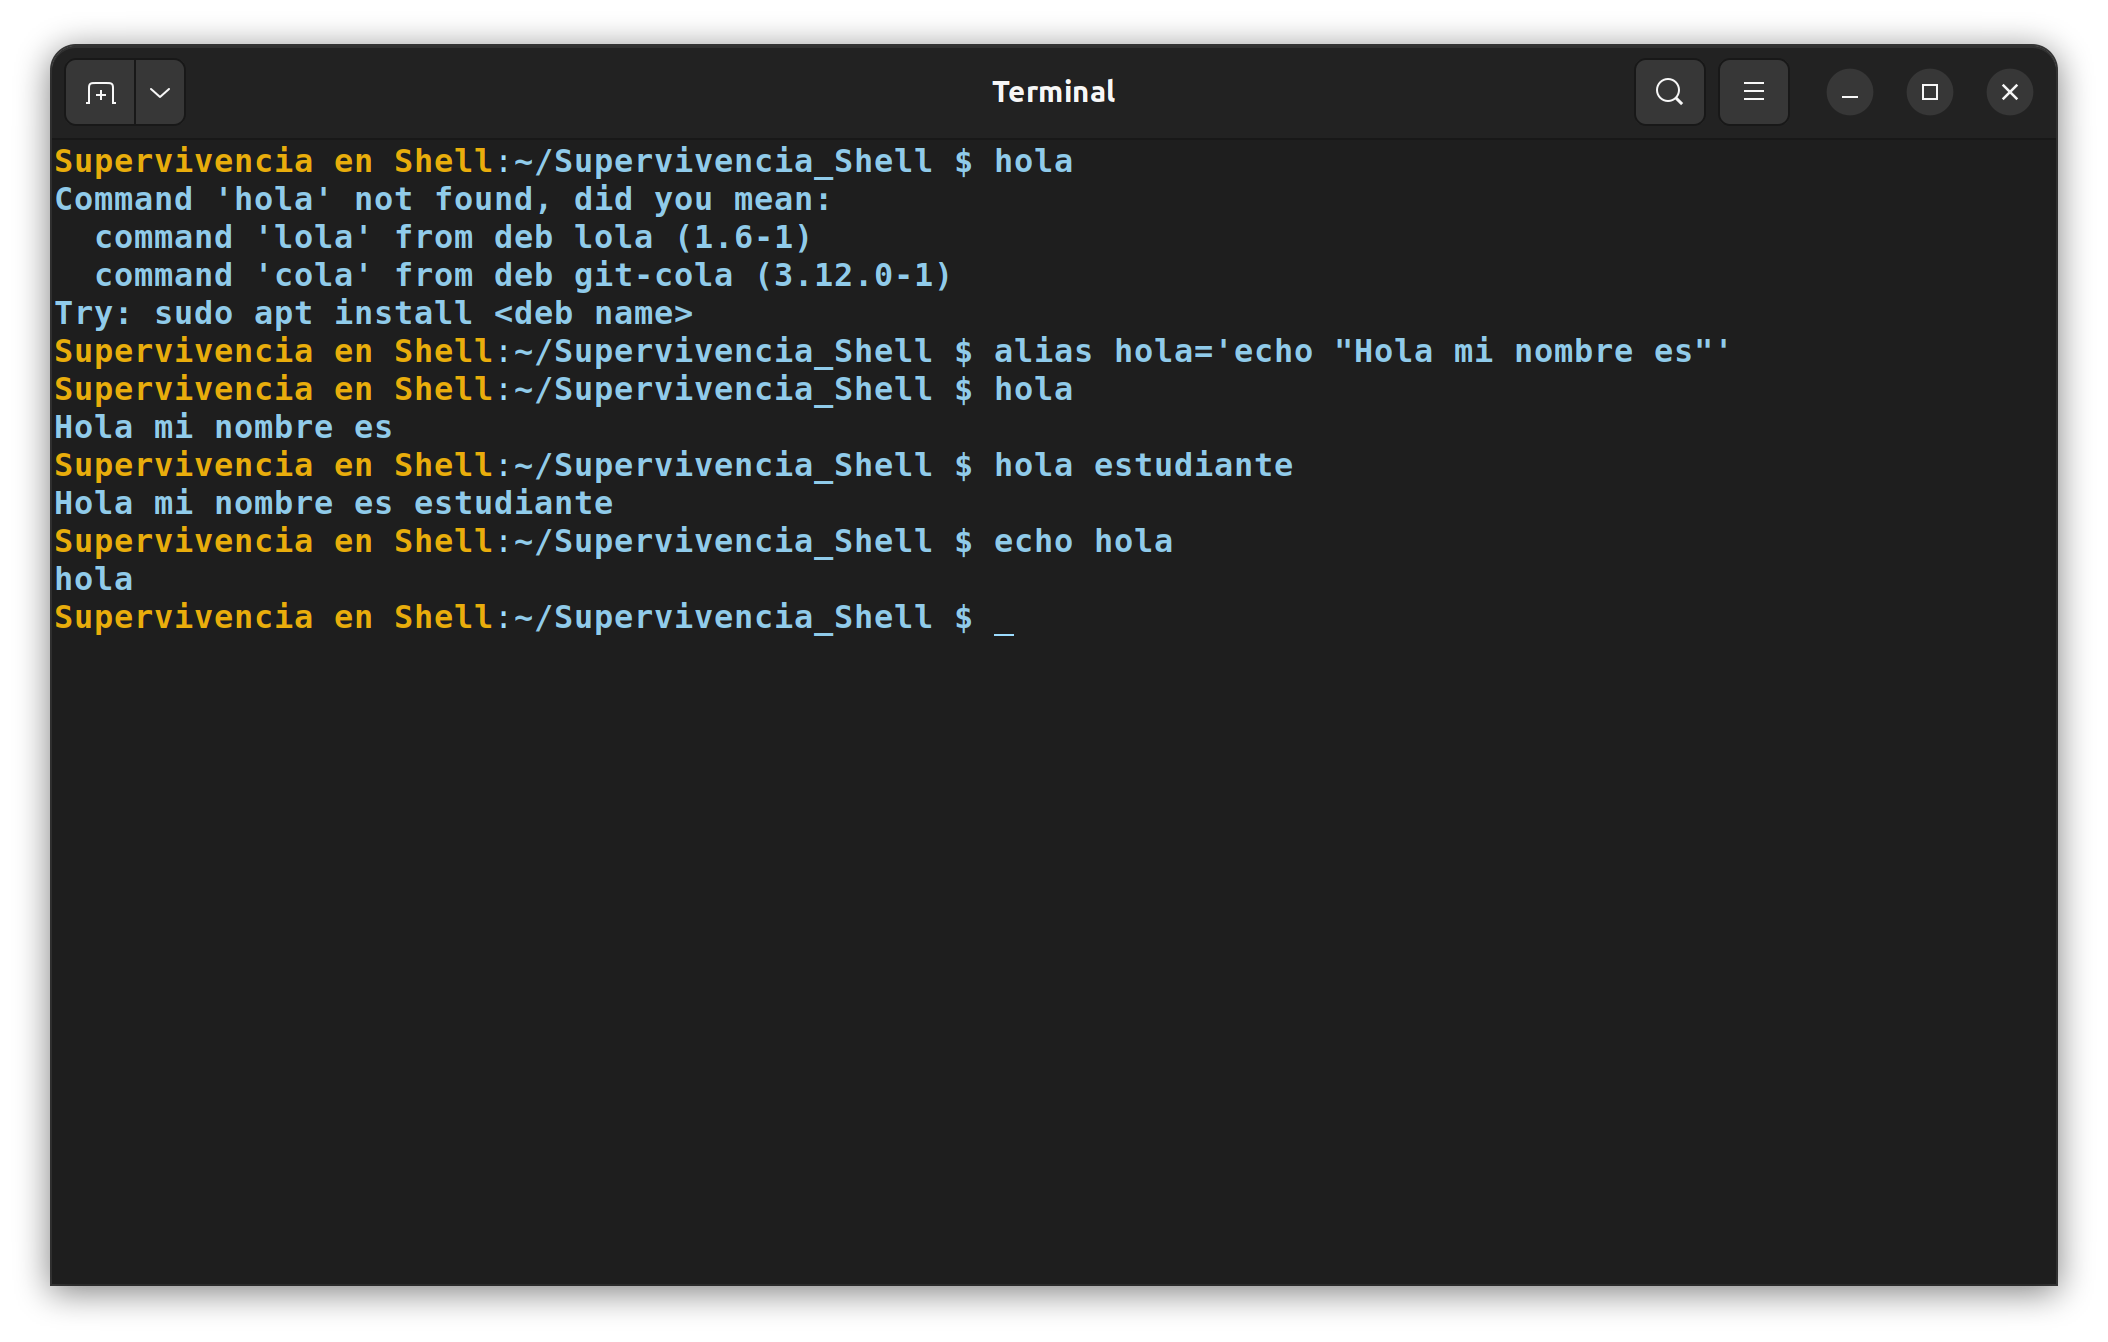
\includegraphics[width=0.55\textwidth]{alias}
		\end{center}
	\end{frame}	

	\begin{frame}
		\frametitle{Uso avanzado: pipes}
		\begin{alertblock}{Conecta la salida de un comando con la entrada del siguiente.}
			command1 $|$ command2 $|$ command3 
		\end{alertblock}
		\begin{center}
			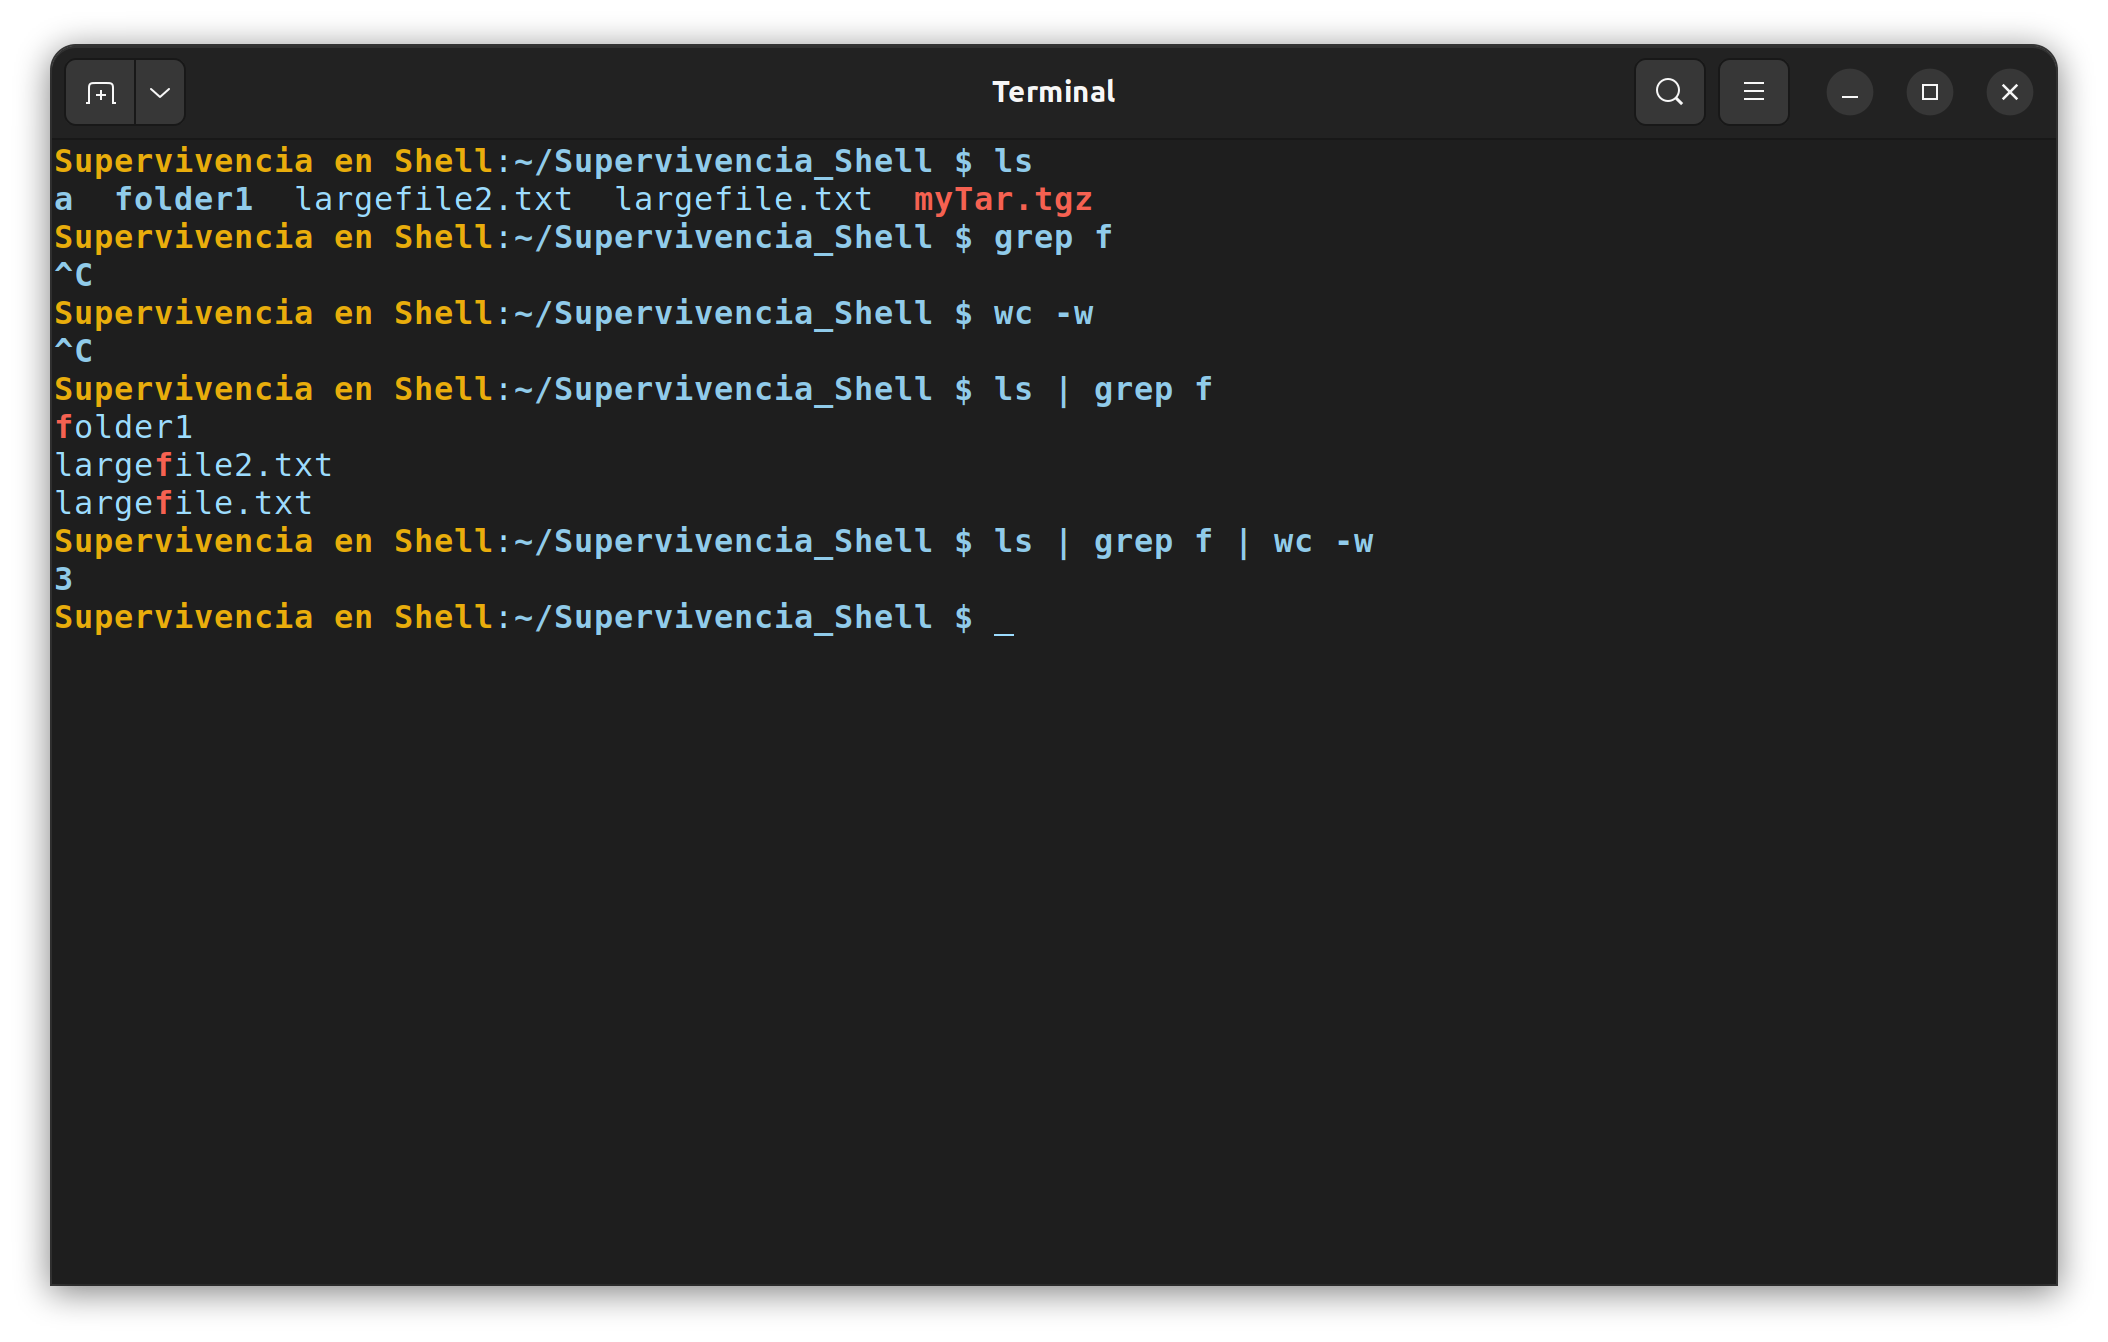
\includegraphics[width=0.55\textwidth]{pipes}
		\end{center}
	\end{frame}
	
	\begin{frame}
		\frametitle{Uso avanzado: redirecciones de salida a ficheros}
		\begin{alertblock}{Redirige la salida de un comando a un fichero.}
			"$>$" Reemplaza los contenidos del fichero.\\
			"$>>$" Añade los contenidos al fichero.
		\end{alertblock}
		\begin{center}
			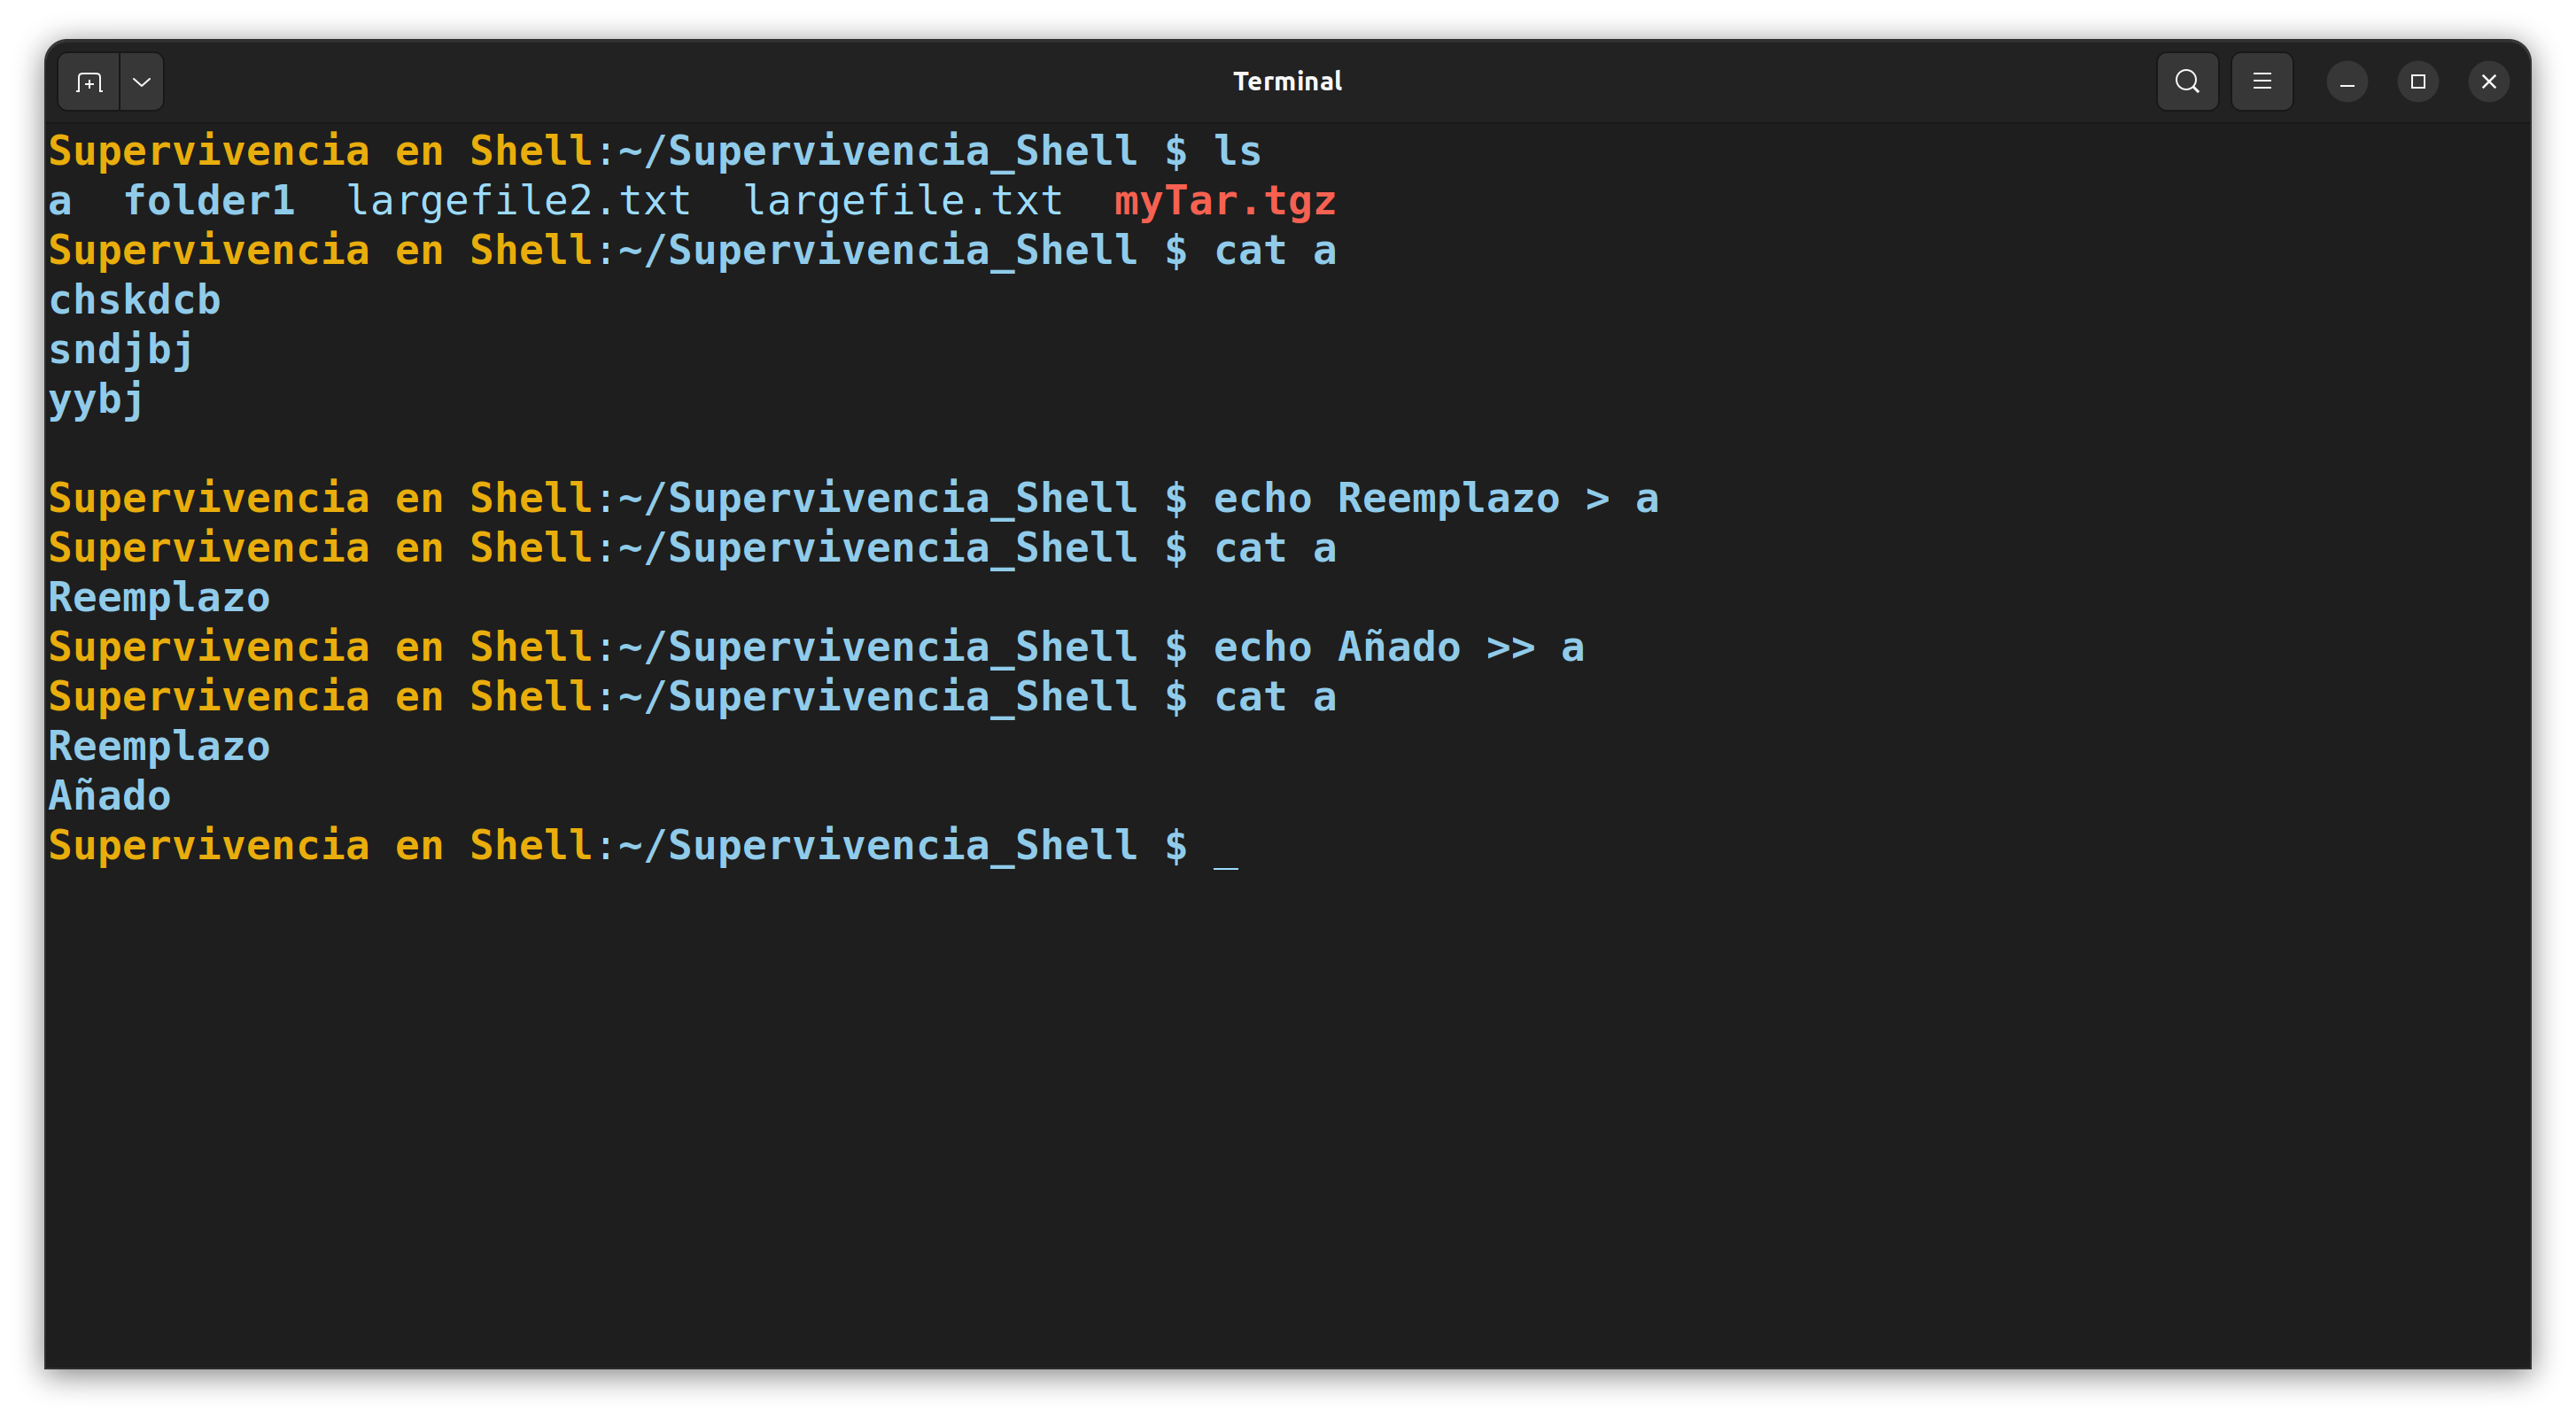
\includegraphics[width=0.55\textwidth]{redir}
		\end{center}
	\end{frame}	

\end{document}